\documentclass[10pt, a4paper]{report}

\usepackage{tikz}

% archivo con las configuraciones del documento y los paquetes usados
\input{settings.tex}

\begin{document}
%===================================================
%                     CARATULA
%===================================================
    \begin{center}

        \thispagestyle{empty}  % Saca la numeracion a la primer pagina

        \includegraphics[scale=0.2]{figs/logoitba2.png}
        \medskip
        
        \textbf{\large{INSTITUTO  TECNOL\'OGICO DE BUENOS AIRES}\normalsize}
        
        \smallskip
        
        \textbf{\large  Departamento de Ciencias Exactas y Naturales}
        
        \smallskip
        \textbf{\large \'Area  Matem\'atica}
      
        \vspace{2 cm}
        
        \textbf{\Large \noindent \textbf{Parciales Resueltos.}}
             
        \vspace{1.5cm}
        
        \large  Material de lectura para alumnos........  \normalsize
    \end{center}
    
    \newpage

%===================================================
%                   INTRODUCCION
%===================================================
    \setcounter{page}{1}
    \begin{center}
        \textbf{ \noindent \textbf{Parciales Resueltos}}
    \end{center}
    \vspace{3cm}
      
    (Pequena explicacion).  Este documento presentaremos distintos ejercicios de parcial....
    \newpage

%===================================================
%                      INDICE
%===================================================
    \tableofcontents
        \pagenumbering{arabic}
        \setcounter{page}{1}
    \vfill
  %  \textcolor{red}{algun tipo de nota explicando detalles de notacion, por ej.} Los símbolos para los vectores serán marcados en negrita minúscula, $\mathbf{v},\;\mathbf{x},\;\mathbf{n},\;\boldsymbol{\sigma}$ etc., y mayúscula los campos vectoriales, $\mathbf{F},\;\mathbf{G},\;\boldsymbol{\Sigma}$, etc. Las matrices estarán en negritas e italicas, $\boldsymbol{D},\;\boldsymbol{H}$, etc.

%===================================================
%                CONTENIDO TEORICO
%===================================================
    \chapter{Contenido teórico. Primera parte}
        \section{Recuerdo de Análisis Matemático 1}
          \begin{definition}
   Se llama \textit{función} a la regla que asigna a cada elemento de un conjunto
    $A$  un y s\'olo un elemento de un conjunto $B$. Tomaremos, en esta secci\'on,  el caso  donde $A, B \subseteq \mathbb{R}.$   La manera habitual de denotar una funci\'on $f$ es $$f: A \subseteq \mathbb{R} \rightarrow B \subseteq \mathbb{R}.$$  A los conjuntos $A$ y $B$  se los llama, respectivamente, \textit{dominio}  y \textit{codominio} de la funci\'on y  la notaci\'on usual para los mismos  es  $A=\text{Dom}(f)$ y $B=\text{Cod}(f)$.
    \label{def:FuncMate1}
\end{definition}


\begin{definition} Dada una funci\'on $f: A \subseteq \mathbb{R} \rightarrow B \subseteq \mathbb{R},$  se llama \textit{imagen} de una función y se nota  $\text{Im}(f)$, a
    al conjunto 
    \begin{equation*}
        \text{Im}(f) = \left\{ y\in B: \exists\;x\in A\:|\:f(x)=y \right\}.    
    \end{equation*}
\end{definition}

\begin{definition}\label{grafm1}
   Dada una función $f: A \subseteq \mathbb{R} \rightarrow B \subseteq \mathbb{R}$ se define la \textit{gráfica} de $f$, y se nota  $\text{Graf}(f)$, al conjunto
    \begin{equation*}
        \text{Graf}(f) = \left\{ (x,y)\in \mathbb{R}^{2}: x \in A \land y=f(x)\right\}.    
    \end{equation*}
\end{definition}


%\textcolor{red}{Aca hay un lio en los ejemplos, la tabla y el grafico no corresponden a la formula. Hacer dos ejemplos completo por separado. }

\begin{example}
    Sea $$f:  [0,\infty]  \subseteq \mathbb{R} \rightarrow  \mathbb{R} \:|\:  f(x)=2x-1$$ tenemos que, $f$ es el nombre de la función, 
    $x$ es la variable independiente de $f$  y $2x-1$ su  fórmula, es decir,  el valor que la asigna $f$ a cada $x \in  [0,+\infty). $ 
    Adem\'as,   $\text{Dom}(f)=  [0,+\infty)$,   $\text{Cod}(f)=  \mathbb{R}$ y $\text{Im}(f)= [-1,+\infty)$ .
    Si se quisiera, se puede hacer una tabla de valores para la función:
    \begin{table}[H]
        \centering
        \begin{tabular}{|c|c|}
            \hline
            $x$ & $y=f(x)=2x-1$ \\ \hline
            -2  & -5        \\ \hline
            -1  & -3        \\ \hline
            0   & -1        \\ \hline
            1   & 1        \\ \hline
            2   & 3        \\ \hline
            \end{tabular}
      \end{table}

      Estos puntos, se pueden graficar sobre un plano cartesiano.
      \begin{figure}[H] 
        \begin{center}
            \begin{tikzpicture}
                \begin{axis}[
                    axis lines = middle,
                    xmin = -2.5, xmax = 2.5,
                    ymin = -5.5, ymax = 3.5,
                    xlabel = {$x$},
                    ylabel = {$y$},
                    domain = -2:2,
                    samples = 100,
                    xtick={-2,-1,1,2},
                    ytick={1,2,3,4},
                    clip=false,
                    ]
                
                    % Define the curves
                    \fill[red] (0,-1) circle (4pt);
                    \fill[red] (-2,-5) circle (4pt);
                    \fill[red] (-1,-3) circle (4pt);
                    \fill[red] (1,1) circle (4pt);
                    \fill[red] (2,3) circle (4pt);
                \end{axis}
            \end{tikzpicture}
        \end{center}
        \caption{Conjunto de puntos pertenecientes a la tabla de valores de $f(x)=2x-1$ posicionados sobre el plano cartesiano.}
        %\label{fig:unitCircle1} % Etiqueta para hacer referencia a la imagen
    \end{figure}
    Además, sabemos que la función corresponde a una función lineal, por lo que, para graficar los infinitos puntos pertenecientes
    a la $\text{Graf}(f)$ podemos unir los anteriores con una recta.
    \begin{figure}[H] 
        \begin{center}
            \begin{tikzpicture}
                \begin{axis}[
                    axis lines = middle,
                    xmin = -2.5, xmax = 2.5,
                    ymin = -5.5, ymax = 3.5,
                    xlabel = {$x$},
                    ylabel = {$y$},
                    domain = -2:2,
                    samples = 100,
                    xtick={-2,-1,1,2},
                    ytick={1,2,3,4},
                    clip=false,
                    ]
                
                    % Define the curves
                    \addplot[name path=A, blue, thick, domain=-2:2] {2*x-1};
                    \fill[red] (0,-1) circle (4pt);
                    \fill[red] (-2,-5) circle (4pt);
                    \fill[red] (-1,-3) circle (4pt);
                    \fill[red] (1,1) circle (4pt);
                    \fill[red] (2,3) circle (4pt);
                \end{axis}
            \end{tikzpicture}
            \end{center}
        \caption{En rojo, los puntos de la tabla de valores. En azul, $\text{Graf}(f)$, con sus infinitos puntos, en el intervalo $[-2,2]$.}
        %\label{fig:unitCircle1} % Etiqueta para hacer referencia a la imagen
    \end{figure}

  \end{example}
\begin{example}  Sea $$f: [-2,2]  \subseteq \mathbb{R} \rightarrow  \mathbb{R} \:|\:  f(x)=x^2$$ 

 Se arma la siguiente tabla de valores, para valores discretos de $x\in [0,2]$:
    \begin{table}[H]
        \centering
        \begin{tabular}{|c|c|}
            \hline
            $x$ & $y=f(x)=x^2$ \\ \hline
            -2  & 4        \\ \hline
            -1  & 1        \\ \hline
            0   & 0        \\ \hline
            1   & 1        \\ \hline
            2   & 4        \\ \hline
            \end{tabular}
      \end{table}
    En este caso, haciendo un análisis de la función, se puede ver que 
    $\text{Dom}(f)=  [-2,2]$,   $\text{Cod}(f)=  \mathbb{R}$ y $\text{Im}(f)= [0,4]$
    Luego, el siguiente conjunto de puntos, se encuentran incluidos en la
    gráfica de la función (que cabe aclarar, tiene infinitos elementos).
    \begin{equation*}
        \left\{ (-2,4),(-1,1),(0,0),(1,1),(2,4) \right\}\subset \text{Graf}(f)
    \end{equation*}
    Este conjunto se puede graficar en el plano coordenado x-y de la siguiente forma.
    \begin{figure}[H] 
        \begin{center}
            \begin{tikzpicture}
                \begin{axis}[
                    axis lines = middle,
                    xmin = -2.5, xmax = 2.5,
                    ymin = 0, ymax = 4.5,
                    xlabel = {$x$},
                    ylabel = {$y$},
                    domain = -2:2,
                    samples = 100,
                    xtick={-2,-1,1,2},
                    ytick={1,2,3,4},
                    clip=false,
                    ]
                
                    % Define the curves
                    \fill[red] (0,0) circle (4pt);
                    \fill[red] (-2,4) circle (4pt);
                    \fill[red] (-1,1) circle (4pt);
                    \fill[red] (1,1) circle (4pt);
                    \fill[red] (2,4) circle (4pt);
                \end{axis}
            \end{tikzpicture}
        \end{center}
        \caption{Subconjunto de los puntos pertenecientes a la $\text{Graf}(f)$ posicionados sobre el plano x-y.}
        %\label{fig:unitCircle1} % Etiqueta para hacer referencia a la imagen
    \end{figure}
    
  
  \textcolor{red}{hacer dos dibujos, el primero solo con los puntos rojos y el segundo con los mismos puntos mas el trazo. Decir algo asi como: por conocimiemto previo sabemos que la manera de unir los puntos es a trav\'es de..... }
  
    Por conocimiento previo, sabemos que la forma de unir estos puntos para graficar $f(x)$ es a través de una parábola. Así, 
    graficando la función como uno lo haría normalmente, en realidad
    se están dibujando los infinitos puntos pertenecientes
    a la $\text{Graf}(f)$ sobre el plano.
        \begin{figure}[H] 
            \begin{center}
                \begin{tikzpicture}
                    \begin{axis}[
                        axis lines = middle,
                        xmin = -2.5, xmax = 2.5,
                        ymin = 0, ymax = 4.5,
                        xlabel = {$x$},
                        ylabel = {$y$},
                        domain = -2:2,
                        samples = 100,
                        xtick={-2,-1,1,2},
                        ytick={1,2,3,4},
                        clip=false,
                        ]
                    
                        % Define the curves
                        \addplot[name path=A, blue, thick, domain=-2:2] {x^2};
                        \fill[red] (0,0) circle (4pt);
                        \fill[red] (-2,4) circle (4pt);
                        \fill[red] (-1,1) circle (4pt);
                        \fill[red] (1,1) circle (4pt);
                        \fill[red] (2,4) circle (4pt);
                    \end{axis}
                \end{tikzpicture}
                \end{center}
            \caption{En rojo, los puntos del subconjunto de la gráfica de la figura anterior. En azul, $\text{Graf}(f)$, con sus infinitos puntos, en el intervalo $[-2,2]$.}
            %\label{fig:unitCircle1} % Etiqueta para hacer referencia a la imagen
        \end{figure}
\end{example}
\begin{definition}
  
  Sea la funci\'on $f: A \subseteq \mathbb{R} \rightarrow B \subseteq \mathbb{R}$. Diremos que
   $f$ es \textit{sobreyectiva} si se cumple que su codominio es igual a su imagen, esto es
   \begin{equation*}
        \text{Cod}(f)=\text{Im}(f).
    \end{equation*}   Es decir que cada elemento del conjunto de salida es la evaluación de la función en al menos un elemento del dominio.

 Diremos que $f$ es   \textit{inyectiva} si a cada elemento en el conjunto imagen le corresponde un único
    valor del  conjunto dominio, esto es,   si  $a,b\in \text{Dom}(f)$, entonces:
     \begin{equation*}
        a=b \iff f(a)=f(b),
    \end{equation*} 

    Finalmente, diremos que $f$  es \textit{biyectiva} cuando es simultáneamente \textit{sobreyectiva} e \textit{inyectiva} a la vez.
\end{definition}

\begin{definition}
    Sea $f(x)$ definida en un intervalo abierto alrededor de $x_0$, excepto posiblemente $x_0$, es decir, en un entorno reducido aldededor del mismo
    $\varepsilon_0(x_0)$, se define el \textit{límite de $f(x)$ cuando x se aproxima a $x_0$}:
    \begin{equation*}
        \lim_{x\to x_0}{f(x)}=L 
    \end{equation*}
    si y solo si
    \begin{equation*}
        \forall \epsilon>0 : \exists \delta >0 : 0<\left\lvert x-x_0 \right\rvert<\delta \Rightarrow \left\lvert f(x) - L\right\rvert < \epsilon 
    \end{equation*}
    \label{def:Limite}
\end{definition}

\begin{obs}{Límites Notables}
    \label{obs:LimitesNotables}
    A continuación se presenta una lista de límites notables que pueden ser de utilidad:

    \begin{minipage}{0.45\textwidth}
        \begin{equation}
            \lim_{x\to 0}{\frac{\sin{x}}{x}}=1
            \label{limNot:sen(x)/x}
        \end{equation}
        \begin{equation}
            \lim_{x\to 0}{\frac{1-\cos{x}}{x}}=0
            \label{limNot:(1-cos(x))/x}
        \end{equation}
        \begin{equation}
            \lim_{x\to 0}{\frac{\exp{kx}-1}{x}}=k
            \label{limNot:(e^{kx}-1)/(x)}
        \end{equation}
    \end{minipage}
    \hfill
    \begin{minipage}{0.45\textwidth}
        \begin{equation}
            \lim_{x\to 0}{\frac{a^{kx}-1}{x}}=k\ln{a}
            \label{limNot:(a^(kx)-1)/(x)}
        \end{equation}
        \begin{equation}
            \lim_{x\to +\infty}{\left( 1+\frac{1}{x} \right)^x}=e
            \label{limNot:e}
        \end{equation}
        \begin{equation}
            \lim_{x\to 0}{\ln{\left(\frac{1+x}{x} \right)}}=1
            \label{limNot:ln(1+x/x)}
        \end{equation}
    \end{minipage}
\end{obs}

\begin{definition}{\textbf{Polinomio de Taylor}}
    Sea $f$ una función con derivades de orden $n$ en $x=a \in \text{Dom}(f)$. Se llama \textit{Polinomio de Taylor} 
    de grado $n$ de la función $f$ en $x=a$, y se simboliza $T_{f,a,n}(x)$, a:
    \begin{equation*}
        T_{f,a,n}(x) = \sum^n_{k=0} \frac{f^{(k)}(a)}{k!}(x-a)^k 
    \end{equation*}
    \label{def:PolTaylor}
\end{definition}
        
         \section{Recuerdo de Álgebra}
           \begin{definition} Se define el  espacio $\mathbb{R}^n$  como el conjunto formado por todas las $n$-uplas de n\'umeros reales ordenados.   Es decir:
    \begin{equation*}
        \mathbb{R}^n = \left\{ \boldsymbol{v} / \boldsymbol{v}=(x_1,x_2,x_3,...,x_n), \; x_i \in \mathbb{R} \;\forall \;   1\leq  i \leq n  \right\}
    \end{equation*}
\end{definition}

\begin{definition}  Sean  $\mathbb{V}$ y $\mathbb{W}$ sub-espacios vectoriales de $\mathbb{R}^n$.  Se  define a  una transformación lineal  como a  una función 
    \begin{equation*}
       \boldsymbol{T}: \mathbb{V} \rightarrow  \mathbb{W}
    \end{equation*}
    que cumple con la condición de linealidad:
    \begin{equation}\label{tl}
        \boldsymbol{T}(\alpha \cdot \boldsymbol{v_1} + \beta \cdot \boldsymbol{v_2})=\alpha \cdot \boldsymbol{T}(\boldsymbol{v_2}) + \beta \cdot \boldsymbol{T}(\boldsymbol{v_2}),
    \end{equation}
    donde $\boldsymbol{v_1},\boldsymbol{v_2} \in \mathbb{V}$ y $\alpha,\beta \in \mathbb{R}$. 
    \label{def:TL}
\end{definition}



\begin{definition} Sean    $\boldsymbol{v}\in\mathbb{R}^n$   no nulo y  $\boldsymbol{x_0}\in\mathbb{R}^n,$  el conjunto $L \subset \mathbb{R}^n $  que cumple  
 \begin{equation*}
      L = \{   \boldsymbol{x} \in\mathbb{R}^n  \:| \:    \boldsymbol{x}=  \lambda \cdot \boldsymbol{v} + \boldsymbol{x_0},  \:  \mbox{  con }  \lambda\in\mathbb{R} \}.
    \end{equation*}  es una recta en $ \mathbb{R}^n $  y a la ecuaci\'on $$ \boldsymbol{x}=  \lambda \cdot \boldsymbol{v} + \boldsymbol{x_0}$$  se  llama  \textbf{expresi\'on vectorial} de la misma.  
    Adem\'as, llamaremos al vector $\boldsymbol{x_0}$ como \textbf{vector posici\'on} (o punto de paso) de la recta y al vector $\boldsymbol{v}$ como \textbf{vector director} de la recta.
 \end{definition}

 \begin{figure}[H]
 \begin{center}
  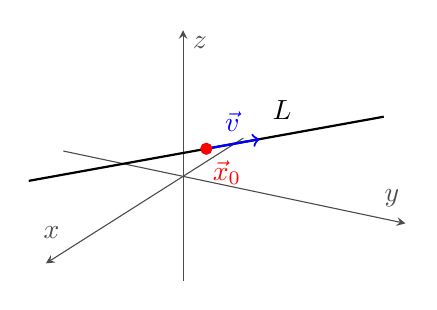
\begin{tikzpicture}
    \begin{axis}[
      view={120}{30},
      axis lines=middle,
      axis line style={black!70},
      label style={black!70},
      enlargelimits=0.5,
      ticks=none,
      xlabel={$x$}, ylabel={$y$}, zlabel={$z$},
      xmin=-1, xmax=8,
      ymin=-1, ymax=4,
      zmin=-1, zmax=2,
    ]
  
      % Punto de paso x_0
      \addplot3[only marks, color=red, mark=*] coordinates {(1, 1, 1)};
      \node at (axis cs:1.3,1.7,0.6) {$\textcolor{red}{\vec{x}_0}$};
  
     
  
      % Recta L: r(t) = x_0 + t * v
      \addplot3[
        domain=-10:10,
        samples=50,
        samples y=0,
        thick,
        black,
        variable=t,
        parametric,
      ] 
      ({1 + 1.5*t}, {1 + 1*t}, {1 + 0.5*t});
      \node at (axis cs:5,4.5,3.2) {$L$};
  
       % Vector director v (desde x_0)
      \addplot3[->, thick, blue] coordinates {(1,1,1) (5.5,4,2.5)};
      \node at (axis cs:3.3,2.5,2.3) {$\textcolor{blue}{\vec{v}}$};
  
    \end{axis}
  \end{tikzpicture}
  \caption{Ejemplo de una recta $L$, con su vector director $\vect{v}$ y punto de paso $\vect{x_0}$.}
  \end{center}
\end{figure}

\begin{definition} Sean    $\boldsymbol{n}\in\mathbb{R}^3$   no nulo  y  $\boldsymbol{x_0}\in\mathbb{R}^3,$  el conjunto $\pi \subset \mathbb{R}^3 $  que cumple  
    \begin{equation*}
      \pi  = \{   \boldsymbol{x} \in\mathbb{R}^3  \:| \:    \boldsymbol{n}\cdot(\boldsymbol{x} - \boldsymbol{x_0}) =0   \}.
    \end{equation*} es un plano en $\mathbb{R}^3$  y a la ecuaci\'on   $$ \boldsymbol{n}\cdot(\boldsymbol{x} - \boldsymbol{x_0}) =0$$  se llama  \textbf{expresi\'on canónica} del mismo.  Adem\'as, llamaremos al vector $\boldsymbol{n}$   como \textbf{vector normal} del plano 
    y al vector  $\boldsymbol{x_0}$ \textbf{punto de paso} del plano. 

    A su vez, también se puede expresar un plano análogamente a la forma propuesta para la recta:
    \begin{equation*}
      \pi  = \{   \boldsymbol{x} \in\mathbb{R}^3  \:| \:    \boldsymbol{x}=\boldsymbol{x_0}+\alpha \boldsymbol{u} + \beta \boldsymbol{u},  \:  \mbox{  con }  \alpha,\beta\in\mathbb{R}    \}.
    \end{equation*} tal que la ecuación
    \begin{equation*}
       \boldsymbol{x}=\boldsymbol{x_0}+\alpha \boldsymbol{u} + \beta \boldsymbol{v}
    \end{equation*}
    se conoce como la \textbf{forma vectorial} del plano. Donde $\boldsymbol{u}$ y $\boldsymbol{v}$ son dos \textbf{vectores paralelos al plano}, que cumplen que $\boldsymbol{v}\times\boldsymbol{u}\shortparallel \boldsymbol{n}$, el vector normal del plano.
    Finalmente, $\alpha$ y $\beta$ son \textbf{parámetros} reales.

 \end{definition}
   
 \begin{figure}[H]
  \begin{center}
    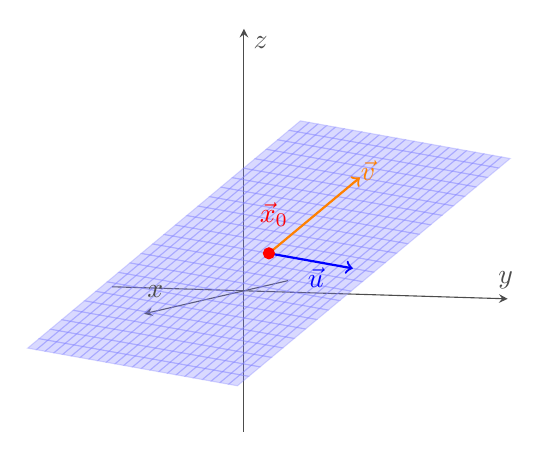
\begin{tikzpicture}
      \begin{axis}[
        view={110}{5},
        axis lines=middle,
        axis line style={black!70},
        label style={black!70},
        enlargelimits=0.5,
        ticks=none,
        xlabel={$x$}, ylabel={$y$}, zlabel={$z$},
        xmin=-1, xmax=8,
        ymin=-1, ymax=5,
        zmin=-1, zmax=4,
      ]
    
        
    
        % Plano generado por x_0 + s*u + t*v
        \addplot3[
          surf,
          opacity=0.3,
          color=blue!50!white,
          shader=flat,
          domain=-5:5,
          domain y=-1.5:1.5,
        ]
        (
          {1 + 1.5*x + 1*y},
          {1 + 1*x + 3*y},
          {1 + 0*x + 2*y}
        );
    
        % Punto de paso x_0
        \addplot3[only marks, color=red, mark=*] coordinates {(1, 1, 1)};
        \node at (axis cs:1.6,1.3,2) {$\textcolor{red}{\vec{x}_0}$};
    
        % Vectores u y v
        \addplot3[->, thick, blue] coordinates {(1,1,1) (7,5,1)};
        \node at (axis cs:4.2,3.2,0.6) {$\textcolor{blue}{\vec{u}}$};
    
        \addplot3[->, thick, orange] coordinates {(1,1,1) (2,4,3)};
        \node at (axis cs:2.2,4.3,3.2) {$\textcolor{orange}{\vec{v}}$};
    
      \end{axis}
    \end{tikzpicture}
   \caption{Ejemplo un plano $\pi$, con su punto de paso $\vect{x_0}$ y vector normal $\vect{n}$.}
   \end{center}
 \end{figure}

 \begin{figure}[H]
  \begin{center}
    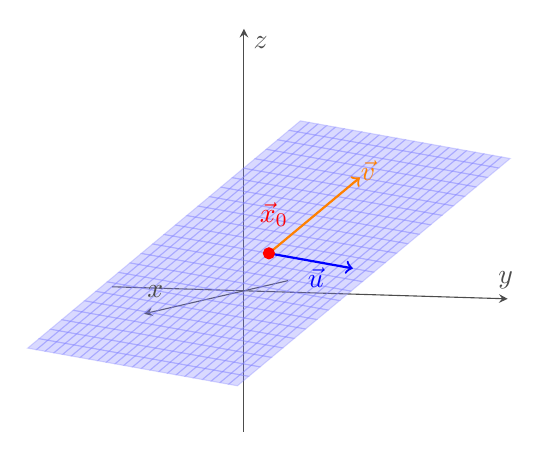
\begin{tikzpicture}
      \begin{axis}[
        view={110}{5},
        axis lines=middle,
        axis line style={black!70},
        label style={black!70},
        enlargelimits=0.5,
        ticks=none,
        xlabel={$x$}, ylabel={$y$}, zlabel={$z$},
        xmin=-1, xmax=8,
        ymin=-1, ymax=5,
        zmin=-1, zmax=4,
      ]
    
        
    
        % Plano generado por x_0 + s*u + t*v
        \addplot3[
          surf,
          opacity=0.3,
          color=blue!50!white,
          shader=flat,
          domain=-5:5,
          domain y=-1.5:1.5,
        ]
        (
          {1 + 1.5*x + 1*y},
          {1 + 1*x + 3*y},
          {1 + 0*x + 2*y}
        );
    
        % Punto de paso x_0
        \addplot3[only marks, color=red, mark=*] coordinates {(1, 1, 1)};
        \node at (axis cs:1.6,1.3,2) {$\textcolor{red}{\vec{x}_0}$};
    
        % Vectores u y v
        \addplot3[->, thick, blue] coordinates {(1,1,1) (7,5,1)};
        \node at (axis cs:4.2,3.2,0.6) {$\textcolor{blue}{\vec{u}}$};
    
        \addplot3[->, thick, orange] coordinates {(1,1,1) (2,4,3)};
        \node at (axis cs:2.2,4.3,3.2) {$\textcolor{orange}{\vec{v}}$};
    
      \end{axis}
    \end{tikzpicture}
   \caption{Ejemplo del mismo plano de la figura anterior, $\pi$, pero con sus vectores directores $\vect{v}$ y $\vect{u}$ y punto de paso $\vect{x_0}$.}
   \end{center}
 \end{figure}


   
  %\textcolor{red}{Agregar forma vectorial del plano}

  
  

\begin{definition} Sean  $(x_0,y_0) \in \mathbb{R}^2$ y $r \in \mathbb{R}_{ > 0}. $

  El conjunto $C \subset \mathbb{R}^2$ que cumple
    \begin{equation*}\label{circ}
    C = \{  (x,y)  \in \mathbb{R}^2 \:|\:   (x-x_0)^2+(y-y_0)^2=r^2 \}
    \end{equation*}  es una circunferencia en el plano. Adem\'as, al vector $(x_0,y_0)$  se lo llama centro y al n\'umero $r$  se lo llama radio de la misma.
   
  El conjunto $D \subset \mathbb{R}^2$ que cumple
    \begin{equation*}
    D = \{  (x,y)  \in \mathbb{R}^2 \:|\:   (x-x_0)^2+(y-y_0)^2 \leq r^2 \}
    \end{equation*}  es un c\'irculo en el plano. Adem\'as, al vector $(x_0,y_0)$  se lo llama centro y al n\'umero $r$  se lo llama radio del mismo.  
   \end{definition}
   \begin{figure}[H]
    \begin{center}
      \begin{tikzpicture}
        \begin{axis}[
          axis lines=middle,
          axis line style={black!70},
          label style={black!70},
          ticks=none,
          xlabel={$x$}, ylabel={$y$},
          xmin=-1, xmax=4,
          ymin=-1, ymax=4,
          width=10cm,
          height=10cm,
        ]
      
          % Centro de la circunferencia
          \def\xo{2}
          \def\yo{2}
          \def\radio{1.5}
      
          % Circunferencia
          \addplot [
            domain=0:360,
            samples=200,
            smooth,
            thick,
            black
          ] ({\xo + \radio*cos(x)}, {\yo + \radio*sin(x)});
          
          % Etiqueta para la circunferencia
          \node at (axis cs:{\xo + \radio + 0.1}, {\yo+1}) {$C$};
      
          % Punto (x_0, y_0)
          \addplot[only marks, mark=*, red] coordinates {(\xo,\yo)};
          \node at (axis cs:{\xo + 0.4}, {\yo + 0.4}) {$\textcolor{red}{(x_0, y_0)}$};

          % Vector radio (desde el centro hacia la derecha)
          \addplot[->, thick, blue] coordinates {(\xo, \yo) ({\xo + \radio}, \yo)};
          \node at (axis cs:{\xo + \radio/2}, {\yo - 0.2}) {$\textcolor{blue}{r}$};
      
        \end{axis}
      \end{tikzpicture}
     \caption{Circunferencia $C$ de radio $r$ y centro $(x_0,y_0)$.}
     \end{center}
   \end{figure}
   
   \begin{figure}[H]
    \begin{center}
      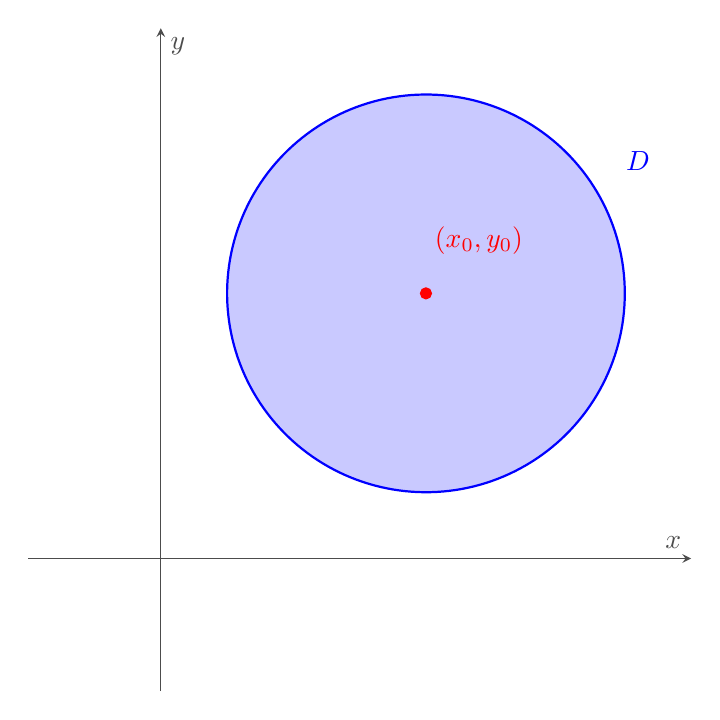
\begin{tikzpicture}
        \begin{axis}[
          axis lines=middle,
          axis line style={black!70},
          label style={black!70},
          ticks=none,
          xlabel={$x$}, ylabel={$y$},
          xmin=-1, xmax=4,
          ymin=-1, ymax=4,
          width=10cm,
          height=10cm,
        ]
      
          % Centro de la circunferencia
          \def\xo{2}
          \def\yo{2}
          \def\radio{1.5}
      
          % Circunferencia rellena
          \addplot [
            domain=0:360,
            samples=200,
            fill=blue!70,
            fill opacity=0.3,
            draw=blue,
            thick,
          ] ({\xo + \radio*cos(x)}, {\yo + \radio*sin(x)});
          
          % Etiqueta para la circunferencia
          \node at (axis cs:{\xo + \radio + 0.1}, {\yo+1}) {$\textcolor{blue}{D}$};
      
          % Punto (x_0, y_0)
          \addplot[only marks, mark=*, red] coordinates {(\xo,\yo)};
          \node at (axis cs:{\xo + 0.4}, {\yo + 0.4}) {$\textcolor{red}{(x_0, y_0)}$};
          
      
        \end{axis}
      \end{tikzpicture}
     \caption{Si se rellena la circunferencia $C$ se obtiene el circulo $D$. Es decir, el círculo $D$ de la figura tiene como borde, o frontera, la circunferencia $C$.}
     \end{center}
   \end{figure}
   
   
\begin{definition}\textbf{Ecuación de la esfera.}
    La cáscara de una esfera (es decir, sólo su superficie exterior, hueca) 
    se expresa como un conjunto $A\subset\mathbb{R}^3$ que cumple
    \begin{equation*}
      S = \{  (x,y,z)  \in \mathbb{R}^3 \:|\:   (x-x_0)^2+(y-y_0)^2+(z-z_0)^2=r^2 \}
    \end{equation*}
    Se tiene $(x_0,y_0,z_0)$ como el centro de la cáscara y $r$ como el radio de la misma.
    Para obtener un conjunto $B\subset\mathbb{R}^3$ que represente la esfera completa, es decir, cáscara y relleno interior, se debe tener
    \begin{equation*}
      V = \{  (x,y,z)  \in \mathbb{R}^3 \:|\:   (x-x_0)^2+(y-y_0)^2+(z-z_0)^2\leq r^2 \}
    \end{equation*}
    Esto es análogo al caso de la circunferencia y el círculo.
\end{definition}

\begin{figure}[H]
  \begin{center}
    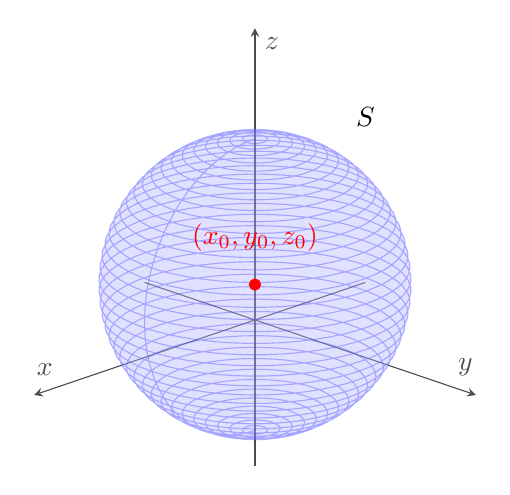
\begin{tikzpicture}
      \begin{axis}[
        view={135}{20},
        axis lines=middle,
        axis line style={black!70},
        label style={black!70},
        ticks=none,
        xlabel={$x$}, ylabel={$y$}, zlabel={$z$},
        xmin=-2, xmax=4,
        ymin=-2, ymax=4,
        zmin=-2, zmax=4,
        width=10cm,
        height=10cm,
      ]
    
        % Centro y radio
        \def\xo{1}
        \def\yo{1}
        \def\zo{1}
        \def\radio{2}
    
        % Esfera con borde visible
        \addplot3[
          domain=0:360,
          y domain=0:180,
          draw=blue!70,
          fill=blue!30,
          opacity=0.4,
          faceted color=blue!60,
          shader=flat,
          samples=60,
          samples y=40,
        ]
        (
          {\xo + \radio * cos(x) * sin(y)},
          {\yo + \radio * sin(x) * sin(y)},
          {\zo + \radio * cos(y)}
        );
    
        % Punto central
        \addplot3[only marks, color=red, mark=*] coordinates {(\xo,\yo,\zo)};
        \node at (axis cs:{\xo + 0.5},{\yo + 0.5},{\zo + 0.9}) {\textcolor{red}{\((x_0, y_0, z_0)\)}};
    
        % Etiqueta para la esfera
        \node at (axis cs:{\xo + \radio + 0.3},{\yo + \radio + 2.3},{\zo+4}) {$S$};
    
      \end{axis}
    \end{tikzpicture}
   \caption{Cáscara de esfera $S$ con centro $(x_0,y_0,z_0)$.}
   \end{center}
 \end{figure}

 \begin{figure}[H]
  \begin{center}
    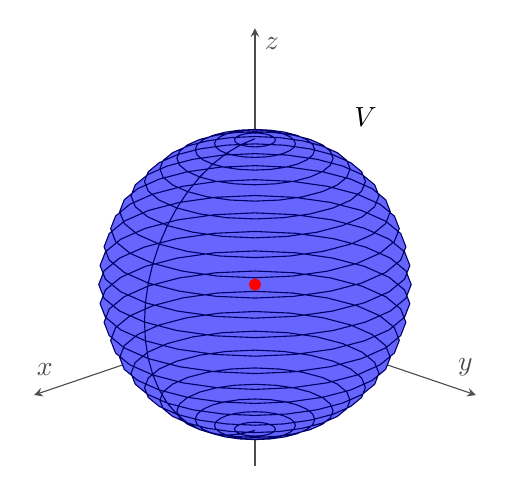
\begin{tikzpicture}
      \begin{axis}[
        view={135}{20},
        axis lines=middle,
        axis line style={black!70},
        label style={black!70},
        ticks=none,
        xlabel={$x$}, ylabel={$y$}, zlabel={$z$},
        xmin=-2, xmax=4,
        ymin=-2, ymax=4,
        zmin=-2, zmax=4,
        width=10cm,
        height=10cm,
      ]
    
        % Centro y radio
        \def\xo{1}
        \def\yo{1}
        \def\zo{1}
        \def\radio{2}
    
        % Esfera con borde visible
        \addplot3[
          faceted color=blue!60,
          draw=blue!40!black,             % sin líneas visibles
          fill=blue!60!white,
          opacity=1,
          shader=interp,
          domain=0:360,
          y domain=0:180,
        ]
        (
          {\xo + \radio * cos(x) * sin(y)},
          {\yo + \radio * sin(x) * sin(y)},
          {\zo + \radio * cos(y)}
        );
    
        % Punto central
        \addplot3[only marks, color=red, mark=*] coordinates {(\xo,\yo,\zo)};
        
    
        % Etiqueta para la esfera
        \node at (axis cs:{\xo + \radio + 0.3},{\yo + \radio + 2.3},{\zo+4}) {$V$};
    
      \end{axis}
    \end{tikzpicture}
   \caption{Esfera rellena $V$, que tiene como cáscara a $S$, de la figura anterior.}
   \end{center}
 \end{figure}
   
         
         \section{Campos vectoriales y escalares}
            

Observacion: \textcolor{red}{(enumerar)}.Si en la definicion \textcolor{red}{(recuerdo de mate 1. poner referencia)} cambiemos  $A \subset \mathbb{R}$ y $B \subset \mathbb{R}$ por $A \subset \mathbb{R}^{n}$ y $B \subset \mathbb{R}^{m}$  obtenemos de manera analoga la siguiente definici\'on.    



\begin{definition} Un campo $\mathbf{F}$ es una funci\'on  tal que
    $\mathbf{F}:A\subseteq \mathbb{R}^n \rightarrow B \subseteq \mathbb{R}^m.$   Si $m=1$ lo llamaremos  \textit{ campo vectorial }  y  si  $m\geq 2$ lo llamaremos   \textit{ campo escalar}. Al igual que en  \textcolor{red}{(recuerdo de mate 1. poner referencia)} a los conjuntos $A$ y $B$  se los llama, respectivamente, \textit{dominio}  y \textit{codominio} del campo $F$ y  la notaci\'on usual para los mismos  es  $A=\text{Dom}( \mathbf{F})$ y $B=\text{Cod}( \mathbf{F})$.   
  \end{definition}
  
  
  
  Notaci\'on:  \textcolor{red}{(enumerar)}  En general,  para nombrar a   campos escalars lo haremos con  letras minúsculas de imprenta y para nombrar a   campos vectorials lo haremos con  letras mayúsculas de imprenta.
  
  \begin{definition}
  Sea   $\mathbf{F}:A\subseteq \mathbb{R}^n \rightarrow B \subseteq \mathbb{R}^m$   un campo vectorial, dado $\boldsymbol{X} \in A$ se puede pensar a  $\mathbf{F}(\boldsymbol{X})$   como la evaluación de $m$ campos escalares en $\boldsymbol{X}$, 
    es decir,
    \begin{equation*}
        \mathbf{F}(\boldsymbol{X})=(f_0(\boldsymbol{X}), f_1(\boldsymbol{X}),..., f_m(\boldsymbol{X})).
    \end{equation*}
  Para $1 \leq i \leq n$,  el campo escalar $f_i: A\subseteq \mathbb{R}^n \rightarrow  \mathbb{R}$ se llama la \textit{i-\'esima componente} de $\mathbf{F}.$
 \end{definition}
  
  
  \begin{definition}
    Sea  $\mathbf{F}:A\subseteq \mathbb{R}^n \rightarrow B \subseteq \mathbb{R}^m$, se define el conjunto im\'agen de $\mathbf{F}$, y se nota $ \text{Img}(\mathbf{F})$, a 
    \begin{equation*}
        \text{Img}(\mathbf{F})=\{\boldsymbol{Y}\in\mathbb{R}^m: \mathbf{F}(\boldsymbol{X})=\boldsymbol{Y}, \boldsymbol{X} \in A\}
    \end{equation*}
  \end{definition}
  
  
    \begin{example}  \label{ej:campoVectorial}
        La función $\boldsymbol{T}:\mathbb{R}^2 \rightarrow \mathbb{R}^3 / \boldsymbol{T}(x,y) = (x+y,x-y,xy)$
        es un campo vectorial. 
       
        \textcolor{red}{decir quies es dominio, imagen, las componentes, y hacer un dibujo del dominio al codominio y sus componentes, revisar que todo lo pedido este definido previamente }
       
        \begin{equation*}
            \boldsymbol{T}(1,1)=(2,0,1)
        \end{equation*}
      
    \end{example}






\begin{example}
        La función $d:\mathbb{R}^3 \rightarrow \mathbb{R} / d(x,y,z) = \sqrt{x^2+y^2+z^2}$
        es un campo escalar.  
    \end{example} 
   
     \textcolor{red}{decir quies es dominio, imagen, las componentes, y hacer un dibujo del dominio al codominio }      
        
       Observacion: \textcolor{red}{ENUMERAR} En particular, si se piensa el vector argumento como un punto en el espacio, $d$ devuelve su distancia euclidea al orígen.
        \begin{equation*}
            \Rightarrow d(1,2,3)=\sqrt{1^2+2^2+3^2}=\sqrt{14}
        \end{equation*}
        \label{ej:campoEscalar}
  


    \begin{example}
    Probar que el campo $T(x,y) = (x+y,x-y,x+y)$  es una transformaci\'on lineal, es decir, que cumple  la condi\'on de   (\ref{def:TL}). Calcular su dominio, Imagen y mostrar sus componetes.
    
     \textcolor{red}{Resolver hacer un dibujo de dominio y codominio}
    
   \end{example}


\begin{definition} Se llaman parametrizaciones a las funciones de la forma $\boldsymbol{\sigma}:A\subseteq\mathbb{R}\rightarrow B\subseteq\mathbb{R}^m$ con $ m>1$.   
\end{definition}
   
   
   Notaci\'on:  \textcolor{red}{(enumerar)}  En general,  a una  parametrización se la suele notar con una letra min\'uscula del alfabeta griego.

    \begin{example} Hallar una parametrizacion del conjuto 
      \begin{equation*}
    C = \{  (x,y)  \in \mathbb{R}^2 \:|\:   x^2+y^2=r^2 \}.
    \end{equation*}  
        
        Para parametrizar una circunferencia, primero pensemos en el circulo unitario.
        En el circulo unitario, la abcisa (coordenada x) de cualquier punto es el coseno del ángulo que forma el eje horizontal con el segmento de radio
        que une el origen con tal punto. Asimismo, el seno del ángulo representa la ordenada (coordenada y).
        \begin{figure}[H] 
            \centering
            \includegraphics[width=0.5\textwidth]{figs/unitCircle1.png} % Cambia esta ruta por la ubicación de tu imagen
            \caption{Coordenadas de los puntos sobre una circunferencia unitaria.}
            \label{fig:unitCircle1} % Etiqueta para hacer referencia a la imagen
        \end{figure}
        Por lo tanto, se propone una parametrización de la circunferencia unitaria de la forma:
        \begin{equation*}
            \boldsymbol{\sigma}:[0,2\pi)\rightarrow\mathbb{R}^2/ \\ \boldsymbol{\sigma}(t)=(\cos{t},\sin{t})
        \end{equation*}
        Así, si se graficase $\text{Img}(\boldsymbol{\sigma})$ como puntos en el plano se obtendría toda la circunferencia unitaria.
        Vale aclarar que se tomó el dominio como cerrado en $0$ y abierto en $2\pi$, para que, puesto que ambos valores de 
        entrada corresponden al mismo punto de salida, la parametrización no tenga "puntos repetidos", es decir, que sea inyectiva 
        (análogo a la inyectividad de funciones de $\mathbb{R}$ a $\mathbb{R}$).
        
         \end{example}
          \begin{example}    
        Hallar una parametrizaci\'on del conjuto 
          \begin{equation*}  
    C = \{  (x,y)  \in \mathbb{R}^2 \:|\:   (x-x_0)^2+(y-y_0)^2=r^2 \}
    \end{equation*} 
         Para contemplar circunferencias de radio distinto de $r$ centro $(0,0)$ vale con multiplicar por el radio a cada componente de la parametrización    \textcolor{red}{referencia}
        Además, para parametrizar aquellas que no estén centradas en el orígen, se desplaza cada punto de salida de la
        parametrización por $(x_0,y_0)$, el centro de la nueva circunferencia.
        Por lo tanto, la parametrización de una circunferencia de radio $r\in\mathbb{R}^+$ centrada en $(x_0,y_0)$ es:
        \begin{equation*}
            \boldsymbol{\sigma}:[0,2\pi)\rightarrow\mathbb{R}^2/ \\ \boldsymbol{\sigma}(t)=(r\cdot\cos{t}+x_0,r\cdot\sin{t}+y_0)
        \end{equation*} 
        
        \textcolor{red}{Agregar la otra manera de  parametrizacion de la circunferencia con el dibujo y la explicacion  }
        
    \end{example}

                  
        \section{Nociones de Topolog\'ia}
            
\textcolor{red}{Falta definicion de distancia, de norma y la relacion entre ellas.  Como ejemplo poner la norma 1 y 2. Graficar algunos mismos conjuntos con diferente normas}



\begin{definition} [Bola de radio $\delta$ y centro $x_o$] \label{def:bola}
    Sean $x_o \in \Rn{n},\;\delta > 0$ y $\text{d}$ una distancia en $\Rn{n}$. La \emph{bola de radio $\delta$ y centro $x_o$}, que denotamos con $B_{\delta}(x_o)$, es el conjunto:
    \[
     B_{\delta}(x_o) = \left\lbrace x \in \Rn{n} : \text{d}(x,x_o) < \delta \right\rbrace.
    \]
    El conjunto
    \[
     B^*_{\delta}(x_o) = B_{\delta}(x_o) - \{ x_o \}
    \]
    es la \emph{bola reducida de radio $\delta$ y centro $x_o$}.
   
   \end{definition}
   
   \begin{definition} [Punto interior, interior de un conjunto] \label{def:interior}
    Sean $A \subset \Rn{n} \text{ y } x_o \in A$. Decimos que $x_o$ es \emph{punto interior} de $A$ si
    \[
     \exists \delta > 0 / B_{\delta}(x_o) \subset A.
    \]
    El \emph{interior} de $A$, que denotamos con $A^{\circ}$, es el conjunto de todos los puntos interiores de $A$:
    \[
    A^{\circ}= \left\lbrace x \in A : x \text{ es punto interior de } A \right\rbrace.
    \]
   \end{definition}
   
   
   \begin{definition} [Conjunto abierto] \label{def:abierto}
       Sea $A \subset \Rn{n}$. Decimos que $A$ es \emph{abierto} si
   \[
        \forall x_o \in \exists \delta > 0 : B_{\delta}(x_o) \subset A.\footnote{\text{i.e.: $A$  es abierto si todos sus puntos son interiores.}}
   \]
   \end{definition}
   
   \begin{propertie}  \label{prop:abierto_int}    Sea  $A \subseteq \Rn{n}$
   
    1.  $A \subseteq  A^{\circ}.$      \:\:\:\:\:\:\:\:\:\:\:\:\:\:\:\:\:\:\:\:                        2.  $\text{   A  es abierto }  \iff   A =  A^{\circ}.$
    \end{propertie}
   
   \begin{definition} [Conjunto cerrado] \label{def:cerrado}
    Sea $A \subset \Rn{n}$. Decimos que $A$ es \emph{cerrado} si su complemento $A^c = \Rn{n} - A$ es abierto.
   \end{definition}
   
   \begin{definition} [Frontera de un conjunto] \label{def:frontera}
    Sea $A \subset \Rn{n}$. La \emph{frontera} de $A$, que denotamos con $\front A$ o $\frontera(A)$, es el conjunto:
    \[
     \front A = \left\lbrace x_o \in \Rn{n} : \forall \delta > 0 \,
     B_{\delta}(x_o) \cap A \ne \emptyset \wedge
     B_{\delta}(x_o) \cap A^c \ne \emptyset \right\rbrace.
    \]
   \end{definition}
   
   \begin{propertie} \label{prop:cerrado_front}
    Un conjunto $A \subset \Rn{n}$ es cerrado si y solo si $\front A \subset A$.
   \end{propertie}
   
   \begin{definition} [Punto de acumulaci\'on] \label{def:pto_acum}
    Sean $A \subset \Rn{n} \text{ y } x_o \in \Rn{n}$. Decimos que $x_o$ es \emph{punto de acumulaci\'on} de $A$ si
    \[
     \forall \delta > 0 \left( B_{\delta}(x_o) - \{ x_o \} \right) \cap A \ne \emptyset. 
    \]
    Denotamos el conjunto de todos los puntos de acumulaci\'on de $A$ con $A'$:
    \[
     A' = \{ x \in \Rn{n} : x \text{ es punto de acumulaci\'on de } A \}.
    \]
   
   \end{definition}
   
   \begin{definition} [Entorno de un punto] \label{def:entorno}
    Sean $N \subset  \Rn{n}$ y $x_o \in \Rn{n}$. Decimos que $N$ es \emph{entorno} de $x_o$ si
    \[
     \exists \delta > 0 : B_{\delta}(x_o) \subset N.
    \]
   \end{definition}
   
   \begin{definition} [Punto aislado] \label{def:pto_ais}
    Sean $A \subset  \Rn{n}$ y $x_o \in A$. Decimos que $x_o$ es \emph{punto aislado} de $A$ si $x_o$ no es punto de acumulaci\'on de $A$.
   \end{definition}
   
   \begin{definition} [Conjunto acotado] \label{def:conj_acotado}
    Sea $A \subset \Rn{n}$. Decimos que $A$ es un \emph{conjunto acotado} si existe $\delta > 0$ tal que la bola de radio $\delta$  centrada en el origen contiene al conjunto $A$, es decir, si $\exists \delta > 0 : A \subset B_{\delta}(\mathbf{0})$.\\
    Equivalentemente, $A$ es un \emph{conjunto acotado} si $\exists \delta > 0, x_o \in \Rn{n} : A \subset B_{\delta}(x_o)$.
   \end{definition}
   
   
   \begin{definition}
    Sea un conjunto $A\subseteq\Rn{n}$. $A$ se llama \textbf{conexo} si dados dos puntos cualquiera de $A$ se los puede unir por una curva continua que este incluida en $A$.
\end{definition}
   
   


%------------------------------------------------------conjunto conexo----------------------------
\begin{definition} [Conjunto conexo] \label{def:conjuntoconexo} Un conjunto \( A \subset \mathbb{R}^n \) es \textbf{conexo} si para cualesquiera dos puntos \( x_0, y_0 \in A \), existe una curva continua \( \gamma : [0,1] \to A \) tal que:

    \[
    \gamma(0) = x_1 \quad \text{y} \quad \gamma(1) = y_1
    \]
    
    
    \begin{center}
        \begin{minipage}{0.45\textwidth}
            \centering
            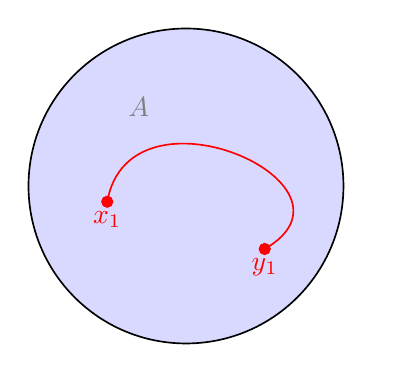
\begin{tikzpicture}
                \draw[fill=blue!15, semithick] (0,0) circle(2);
                \filldraw[red] (-1,-0.2) circle (2pt) node[below] {\(x_1\)};
                \filldraw[red] (1,-0.8) circle (2pt) node[below] {\(y_1\)};
                \draw[semithick,-,red] (-1,-0.2) to[out=80,in=30,looseness=2] (1,-0.8);
                \draw node at (-0.6,1) {\textcolor{gray}{$A$}};
            \end{tikzpicture}
        \end{minipage}
        \hspace{1cm} % espacio entre figuras
        \begin{minipage}{0.45\textwidth}
            \centering
            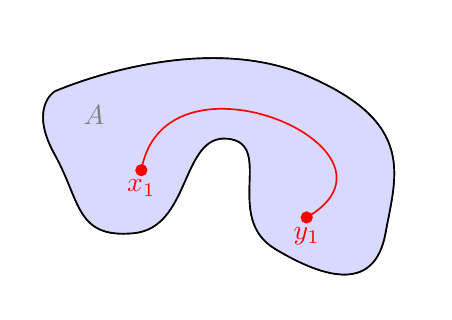
\begin{tikzpicture}
       
                % Plane R^2 on the right
               
                    \draw[semithick]
                        plot[smooth,tension=1.2] coordinates {(-0.2,0.8) (3,1) (4,-1) (2.6,-1.2)(2,0.2) (0.8,-1) (-0.2,0)(-0.2,0.8)};
                    
                    \filldraw[fill=blue!15, semithick]
                        plot[smooth, tension=1.2] coordinates {(-0.2,0.8) (3,1) (4,-1) (2.6,-1.2)(2,0.2) (0.8,-1) (-0.2,0)(-0.2,0.8)};
                        % \foreach \point in {(1,0.6), (3,0), (2.5,-1.5), (1,-1), (0.2,0.1), (1,0.6)} {
                        % \node at \point [circle,fill,inner sep=1pt] {};
                        % }
                    \filldraw[red] (0.9,-0.2) circle (2pt) node[below] {\(x_1\)};
                    \filldraw[red] (3,-0.8) circle (2pt) node[below] {\(y_1\)};
                    \draw[semithick,-,red] (0.9,-0.2) to[out=80,in=30,looseness=2] (3,-0.8);
                    \draw node at (0.3,0.5) {\textcolor{gray}{$A$}};
                    
            
            \end{tikzpicture}
        \end{minipage}
        \end{center}
        \begin{center}
        
\begin{tikzpicture}
            \node at (1.5,-2) {Conjuntos \textbf{conexos}};
        \end{tikzpicture}
        \end{center}
    \end{definition}
    
    %------------------------------------------------------conjunto conexo----------------------------
    \begin{definition} [Conjunto convexo] \label{def:conjuntoconvexo}Un subconjunto \( A \subseteq \mathbb{R}^n \) es \textbf{convexo} si para cualesquiera dos puntos \( x, y \in A \), el segmento que los une está completamente contenido en \( A \):
        \[
        \forall x_1,y_1, \quad \lambda x + (1 - \lambda)y \in A \quad \text{para todo } \lambda \in [0,1].
        \]
        
    
    
    
    
        \begin{center}
            \begin{minipage}{0.45\textwidth}
                \centering
                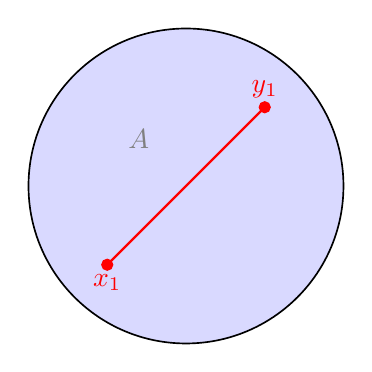
\begin{tikzpicture}
                    \draw[fill=blue!15, semithick] (0,0) circle(2);
                    \filldraw[red] (-1,-1) circle (2pt) node[below] {\(x_1\)};
                    \filldraw[red] (1,1) circle (2pt) node[above] {\(y_1\)};
                    \draw[thick, red, domain=-1:1] plot (\x, {\x});
                    \draw node at (-0.6,0.6) {\textcolor{gray}{$A$}};
                \end{tikzpicture}
            \end{minipage}
            \hspace{1cm} % espacio entre figuras
            \begin{minipage}{0.45\textwidth}
                \centering
                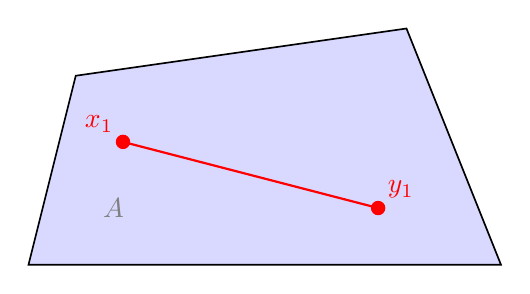
\begin{tikzpicture}[scale=1.2]
                    \filldraw[fill=blue!15, semithick] (-1.5,0) -- (3.5,0) -- (2.5,2.5) -- (-1,2) -- cycle;
                    \draw[thick, red] (-0.5,1.3) -- (2.2,0.6);
                    \filldraw[red] (-0.5,1.3) circle (2pt) node[above left] {\(x_1\)};
                    \filldraw[red] (2.2,0.6) circle (2pt) node[above right] {\(y_1\)};
                    \draw node at (-0.6,0.6) {\textcolor{gray}{$A$}};
                \end{tikzpicture}
            \end{minipage}
            \end{center}
            \begin{center}
            
\begin{tikzpicture}
                \node at (1.5,-2) {Conjuntos \textbf{convexos}};
            \end{tikzpicture}
    
            \end{center}
            \begin{center}
                \begin{minipage}{0.45\textwidth}
                    \centering
                    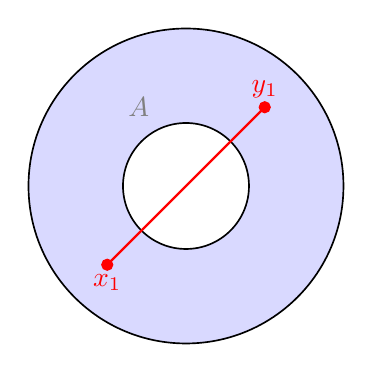
\begin{tikzpicture}
                        % Círculo exterior (azul claro) \draw[fill=blue!15, semithick] (0,0) circle(2);
                        \draw[fill=blue!15, semithick] (0,0) circle(2);
                        
                        % Círculo interior (blanco, para el hueco)
                        \draw[fill=white, semithick] (0,0) circle(0.8);
                        
                        \filldraw[red] (-1,-1) circle (2pt) node[below] {\(x_1\)};
                        \filldraw[red] (1,1) circle (2pt) node[above] {\(y_1\)};
                        \draw[thick, red, domain=-1:1] plot (\x, {\x});
                        
                        % Letra A
                        \draw node at (-0.6,1) {\textcolor{gray}{$A$}};
                    \end{tikzpicture}
                \end{minipage}
                \hspace{1cm} % espacio entre figuras
                \begin{minipage}{0.45\textwidth}
                    \centering
                    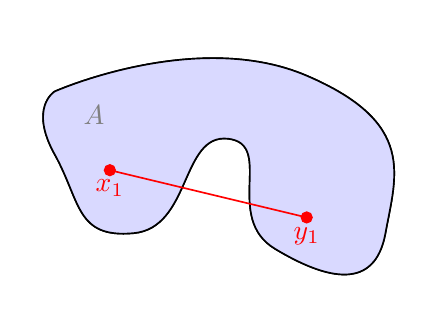
\begin{tikzpicture}
               
                        % Plane R^2 on the right
                       
                            \draw[semithick]
                                plot[smooth,tension=1.2] coordinates {(-0.2,0.8) (3,1) (4,-1) (2.6,-1.2)(2,0.2) (0.8,-1) (-0.2,0)(-0.2,0.8)};
                            
                            \filldraw[fill=blue!15, semithick]
                                plot[smooth, tension=1.2] coordinates {(-0.2,0.8) (3,1) (4,-1) (2.6,-1.2)(2,0.2) (0.8,-1) (-0.2,0)(-0.2,0.8)};
                                % \foreach \point in {(1,0.6), (3,0), (2.5,-1.5), (1,-1), (0.2,0.1), (1,0.6)} {
                                % \node at \point [circle,fill,inner sep=1pt] {};
                                % }
                                \filldraw[red] (0.5,-0.2) circle (2pt) node[below] {\(x_1\)};
                                \filldraw[red] (3,-0.8) circle (2pt) node[below] {\(y_1\)};
                                \draw[semithick, red] (0.5,-0.2) -- (3,-0.8); % Línea recta
                            \draw node at (0.3,0.5) {\textcolor{gray}{$A$}};
                            
                    
                    \end{tikzpicture}
                \end{minipage}
                \end{center}
                \begin{center}
                
\begin{tikzpicture}
                    \node at (1.5,-2) {Conjuntos \textbf{NO convexos}};
                \end{tikzpicture}
                \end{center}
    \end{definition}
    
    %------------------------------------------------------conjunto simplemente conexo----------------------------
    \vspace{0.5cm}
    \begin{definition}[Conjunto conexo] \label{def:conjuntoconexo}
    Un conjunto \( A \subset \mathbb{R}^2 \) es \textbf{simplemente conexo} si es conexo y todo lazo cerrado dentro de \( A \) puede ser continuamente deformado a un punto, sin salir de \( A \).
    
    \vspace{0.3cm} % Pequeño espacio entre el texto y las figuras
    
    \begin{center}
        \begin{minipage}{0.45\textwidth}
            \centering
            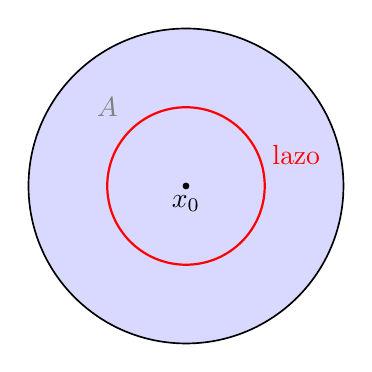
\begin{tikzpicture}
                \draw[fill=blue!15, semithick] (0,0) circle(2);
                \draw[red, thick] (0,0) circle(1);
                \node at (-1,1) {\textcolor{gray}{$A$}};
                \node at (1.4,0.4) {\textcolor{red}{lazo}};
                \filldraw[black] (0,0) circle (1pt) node[below] {\(x_0\)};
            \end{tikzpicture}
        \end{minipage}
        \hspace{1cm}
        \begin{minipage}{0.45\textwidth}
            \centering
            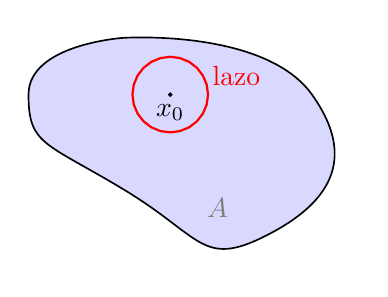
\begin{tikzpicture}[scale=1.2]
                \filldraw[fill=blue!15, semithick]
                    plot[smooth, tension=1.2] coordinates {(1,0.6) (3,0) (2.5,-1.5) (1,-1) (0,0) (1,0.6)};
                \draw[thick, red, domain=0:360] plot ({1.5 + 0.4*cos(\x)}, {0 + 0.4*sin(\x)});
                \node at (2,-1.2) {\textcolor{gray}{$A$}};
                \node[red] at (2.2,0.2) {lazo};
                \filldraw[black] (1.5,0) circle (0.5pt) node[below] {\(x_0\)};
            \end{tikzpicture}
        \end{minipage}
    \end{center}
    
    \vspace{0.3cm} % Pequeño espacio antes de la etiqueta
    
    \begin{center}
        
\begin{tikzpicture}
            \node at (1.5,-2) {Conjuntos \textbf{simplemente conexos}};
        \end{tikzpicture}
    \end{center}
    
    \begin{center}
        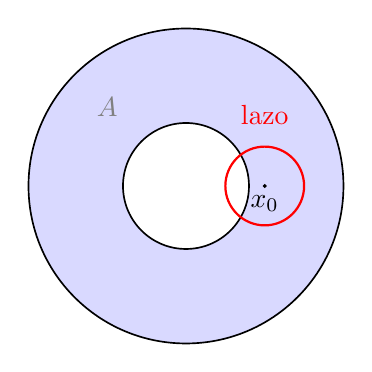
\begin{tikzpicture}
            % Círculo exterior (azul claro) \draw[fill=blue!15, semithick] (0,0) circle(2);
            \draw[fill=blue!15, semithick] (0,0) circle(2);
            
            % Círculo interior (blanco, para el hueco)
            \draw[fill=white, semithick] (0,0) circle(0.8);
            
            \draw[red, thick] (1,0) circle(0.5);
                \node at (-1,1) {\textcolor{gray}{$A$}};
                \node at (1,0.9) {\textcolor{red}{lazo}};
                \filldraw[black] (1,0) circle (0.5pt) node[below] {\(x_0\)};
        \end{tikzpicture}
        \end{center}
        \begin{center}
            
\begin{tikzpicture}
                \node at (1.5,-2) {Conjunto \textbf{NO simplemente conexo}};
            \end{tikzpicture}
        \end{center}
    \end{definition}
    
    
    
    
    
    
    
    
    
    
    
   
   
   
      
        \section{Gráficas}
            \begin{obs} Si en la \autoref{def:grafm1} cambiamos  $A \subseteq \mathbb{R}$ por $A \subseteq \mathbb{R}^{n}$  obtenemos de manera an\'aloga la siguiente definici\'on.    
\end{obs}



\begin{definition}  \label{def:grafica}
 
 Sea \( f: A \subset \mathbb{R}^n \); se define la \textit{gráfica de $f$ }, y se nota $\text{Graf}(f)$,  a
 \[
\text{Graf}(f)=\{(x_1,x_2,...,x_n,x_{n+1})\in \mathbb{R}^{n+1} \;|\; (x_1,x_2,...,x_n) \in A \land f(x_1,x_2,...,x_n)=x_{n+1} \}
 \]

\end{definition}
\begin{obs}  Si \( f: A \subset \mathbb{R}^n \) entonces $\text{Graf}(f) \subset \mathbb{R}^{n+1}.$
\end{obs}

\begin{obs}  Dada la  anterio observaci\'onr y con el objetivo de poder dibujar,  nos detendremos especialmente en el caso de gr\'aficas de  campos  $f: A\subseteq \mathbb{R}^2 \rightarrow \mathbb{R},$ cuya definici\'on se desprende automaticamente  de  (\ref{def:grafica}), o sea el caso
 \[
\text{Graf}(f)=\{(x,y,z)\in \mathbb{R}^3 \;|\;(x,y)\subseteq A \land z=f(x,y) \}.
 \]
\end{obs}



            
        \section{Conjuntos de nivel}
            
\begin{definition} [Conjunto de nivel] 
\label{def:conjunto de nivel}
 \mbox{}
 
Sea $f: U\subset\Rn{n}\rightarrow\R$ y sea $c \in \R$, se define  el conjunto de nivel de $f$ de nivel  $c$, y se nota $C(c,f)$,  a  
\[
C(c,f)=\{ x \in U \backslash f (x)=c \}.
 \]





Es decir,  $C(c,f)$ son aquellos puntos $x\in\ U$ para las cuales $f(x)=c$, o dicho de otra manera,  $C(c,f)$ es la preimagen de $c$ por $f$.   Si $n=2$ hablamos de curva de nivel  y si $n=3$  hablamos de superficie de nivel  

Observaci\'on: \textcolor{red}{Enumerar}   Si $f: A\subseteq\Rn{n}\rightarrow\R$ entonces $C(c,f)  \subset \mathbb{R}^{n}.$



\begin{example}   Sea  el campo  $f: \mathbb{R}^{2} \rightarrow \mathbb{R} \:|\:  f(x,y)=x^2+y^2.$
\end{example}
1. Calcular y graficar los conjuntos de nivel de $f$.

2. Hacer un gr\'afico de  $graf(f)$.



Observemos que, dado $c \in \mathbb{R}$: 
 $$C(c,f)=\{(x,y) \in U \backslash   x^2+y^2  =c \}.$$
 Tomando, para ilustrar,  $c=0$, $c=1$ y $c=4$, quedando (ver (\ref{circ})) 
 \[
C(0,f)=\{(x,y) \in U \backslash x^2+y^2=0 \}
\]
 \[
C(1,f)=\{(x,y) \in U \backslash x^2+y^2=1 \}
\]
 \[
C(4,f)=\{(x,y) \in U \backslash x^2+y^2=4 \}
 \]

\begin{figure}[h!] % El entorno figure te permite incluir imágenes
    \centering
    \includegraphics[width=0.5\textwidth]{figs/conjunto1_r.png} % Cambia esta ruta por la ubicación de tu imagen
    \caption{Conjuntos de nivel}
    \label{fig:ejemplo} % Etiqueta para hacer referencia a la imagen
\end{figure}

En general, podemos determinar: 

   \[
        C(c,f)=
        \begin{dcases}
           \textnormal{Circunferencia centrada en (0,0) de radio} \sqrt{c},  & \textnormal{si}:  c>0 \\
(0,0)  & \textnormal{si}:\ c=0\\
\emptyset  & \textnormal{si}:\ c<0\\
        \end{dcases}
    \]

\textcolor{red}{Aca ``dibujar'' los conjuntos de nivel en $\mathbb{R}^{3}$ y notar que no es suficinte para graficar.}  


\textcolor{red}{Definir cortes transversales y dibujarlos.}


\begin{figure}[h!] % El entorno figure te permite incluir imágenes
    \centering
    \includegraphics[width=0.5\textwidth]{figs/conjunto1_r3.png} % Cambia esta ruta por la ubicación de tu imagen
    \caption{graf(f)}
    \label{fig:ejemplo} % Etiqueta para hacer referencia a la imagen
\end{figure}



 

\begin{example}   Sea  el campo  $g: \mathbb{R}^{2} \rightarrow \mathbb{R} \:|\:  g(x,y) = \sqrt{x^2+y^2}.$
\end{example}
1. Calcular y graficar los conjuntos de nivel de $g$.

2. Hacer un gr\'afico de  $graf(g)$.


\textcolor{red}{Resolver identico al ejercicio  anterior.}  



: Se toma la funcion $f(x,y)=\sqrt{x^2+y^2}$, donde empezamos a analizar los distintos conjuntos de nivel, tomando $c$ con diferentes constantes
 \[
C(0,f)=\{(x,y) \in U \backslash \sqrt{x^2+y^2}=0 \}
\]
 \[
C(1,f)=\{(x,y) \in U \backslash \sqrt{x^2+y^2}=1 \}
\]
 \[
C(2,f)=\{(x,y) \in U \backslash \sqrt{x^2+y^2}=2 \}
 \]

\begin{figure}[h!] % El entorno figure te permite incluir imágenes
    \centering
    \includegraphics[width=0.5\textwidth]{figs/conjunto2_r2.png} % Cambia esta ruta por la ubicación de tu imagen
    \caption{Conjuntos de nivel}
    \label{fig:ejemplo} % Etiqueta para hacer referencia a la imagen
\end{figure}

En general, podemos determinar: 

   \[
        C(c,f)=
        \begin{dcases}
           \textnormal{Circunferencia centrada en (0,0) de radio} c,  & \textnormal{si}:  c>0 \\
(0,0)  & \textnormal{si}:\ c=0\\
\emptyset  & \textnormal{si}:\ c<0\\
        \end{dcases}
    \]
\begin{figure}[h!] % El entorno figure te permite incluir imágenes
    \centering
    \includegraphics[width=0.5\textwidth]{figs/conjunto2_r3.png} % Cambia esta ruta por la ubicación de tu imagen
    \caption{Conjuntos de nivel y graf(f)}
    \label{fig:ejemplo} % Etiqueta para hacer referencia a la imagen
\end{figure}

De esta manera, considerando la definicion de gráfica de una funci\'on, podemos representar la misma en $\Rn{3}$ tomando  la ecuaci\'on de la parte superior de un cono: $z=\sqrt{x^2+y^2}$



\textcolor{red}{Corregir esta observaci\'on. esta mal escrito, quien es la funci\'on f?}


Observaci\'on \textcolor{red}{enumerar}:Dada la  ecuaci\'on $z^2=x^2+y^2$ al despejar z obtenemos $|z|=\sqrt{x^2+y^2}$ obtendriamos que: 
 \[
        C(c,f)=
        \begin{dcases}
           \textnormal{Circunferencia centrada en (0,0) de radio} c,  & \textnormal{si}:  c>0 \\
(0,0)  & \textnormal{si}:\ c=0\\
\textnormal{Circunferencia centrada en (0,0) de radio} c,  & \textnormal{si}:\ c<0\\
        \end{dcases}
    \]

De esta manera, considerando la definicion de gráfica de una funcion, podemos representar la misma en $\Rn{3}$ tomando  la ecuacion del cono: $z^2=x^2+y^2$

\begin{figure}[h!] % El entorno figure te permite incluir imágenes
    \centering
    \includegraphics[width=0.5\textwidth]{figs/conjunto3_r3.png} % Cambia esta ruta por la ubicación de tu imagen
    \caption{Conjuntos de nivel y graf(f)}
    \label{fig:ejemplo} % Etiqueta para hacer referencia a la imagen
\end{figure}


\textcolor{red}{Mejorar la figura, no se llega a apreciar el cono completo}

\end{definition}

         
       \section{L\'imite de Funciones}
          \label{sec:limites}
\begin{definition} [L\'imite] \label{def:limite}
Sean $f:A \subset \Rn{n} \to \Rn{m}$ una funci\'on, $L \in \Rn{m}$ y $x_0$ un punto de acumulaci\'on de $A$. Decimos que \emph{el l\'imite de $f$ para $x$ tendiendo a $x_o$ es $L$} o que \emph{$f$ tiende a $L$ cuando $x$ tiende a $x_o$}
si
\[
 \forall \varepsilon > 0 \, \exists \delta > 0 / f(x) \in B_{\varepsilon}(L) \, \forall 
 x \in B_{\delta}^*(x_o) \cap A.
\]

En este caso, utilizamos la notaci\'on
\[
 f(x) \xrightarrow[x \to x_o]{} L \quad \text{o} \quad \lim_{x \to x_o} f(x) = L.
\]
\begin{obs} Si $f$ es un \emph{campo escalar} (es decir, si en la definici\'on \eqref{def:limite} es $m = 1$), la condici\'on 
 \[
 \forall \varepsilon > 0 \, \exists \delta > 0 / f(x) \in B_{\varepsilon}(L) \, \forall 
 x \in B_{\delta}^*(x_o) \cap A
\]
es equivalente a 
\[
 \forall \varepsilon > 0 \, \exists \delta > 0 / \abs{ f(x) - L } < \varepsilon \, \forall 
 x \in B_{\delta}^*(x_o) \cap A.
\]
\end{obs}

\begin{obs} La definici\'on de l\'imite puede expresarse equivalentemente en t\'erminos de distancias o de normas:
\begin{itemize} 
 \item Sean $f:A \subset \Rn{n} \to \Rn{m}$ una funci\'on, $L \in \Rn{m}$ y $x_0$ un punto de acumulaci\'on de $A$. Decimos que \emph{el l\'imite de $f$ para $x$ tendiendo a $x_o$ es $L$} o que \emph{$f$ tiende a $L$ cuando $x$ tiende a $x_o$} si
\[
 \forall \varepsilon > 0 \, \exists \delta > 0 / \dis_m {(f(x),L)} < \varepsilon \, \forall 
 x\in A : 0 < \dis_n {(x,x_o)} < \delta,
\] 
donde $\dis_n$ y $\dis_m$ son las distancias en $\Rn{n}$ y $\Rn{m}$, respectivamente.

 \item Sean $f:A \subset \Rn{n} \to \Rn{m}$ una funci\'on, $L \in \Rn{m}$ y $x_0$ un punto de acumulaci\'on de $A$. Decimos que \emph{el l\'imite de $f$ para $x$ tendiendo a $x_o$ es $L$} o que \emph{$f$ tiende a $L$ cuando $x$ tiende a $x_o$} si
\[
 \forall \varepsilon > 0 \, \exists \delta > 0 / \norm{f(x) - L}_m < \varepsilon \, \forall 
 x\in A : 0 < \norm{x - x_o}_n < \delta,
\] 
donde $\norm{\cdot}_n$ y $\norm{\cdot}_m$ son las normas en $\Rn{n}$ y $\Rn{m}$, respectivamente.
\end{itemize}
\end{obs}

\end{definition}


\begin{example} Probar, usando la definici\'on, los siguientes l\'imites
 
 \[
  \lim_{(x,y) \to (0,0)} \frac{x^2  y}{x^2 + y^2} = 0.
 \]

 \[
  \lim_{(x,y) \to (0,0)} \frac{x^2 \sin( y)}{x^2 + y^2} = 0.
 \]


\textcolor{red}{mejorar los espacios. Resolver los ejemplos. Hacer menci\'on de los cotas utiles}


\end{example}


\begin{theorem}\textbf{Unicidad del l\'imite.} \label{teo:unicidad_limite}
\mbox{}

Sean $f:A \subset \Rn{n} \to \Rn{m}$ una funci\'on, $x_0$ un punto de acumulaci\'on de $A$ y $L_1, L_2 \in \Rn{m}$ tales que 
\[
 f(x) \xrightarrow[x \to x_o]{} L_1 \quad \wedge \quad f(x) \xrightarrow[x \to x_o]{} L_2.
\]
Entonces $L_1 = L_2$.
\begin{proof}
\mbox{}

Las ideas utilizadas en la demostraci\'on de este teorema son las que siguen.\\
Como 
\[
 f(x) \xrightarrow[x \to x_o]{} L_1,
\]
dado $\varepsilon > 0$ existe alg\'on $\delta_1 > 0$ tal que cada punto $x \in B_{\delta_1}^*(x_o) \cap A$ se aplica a trav\'es de $f$ en alg\'on punto de la bola de centro $L_1$ y radio $\varepsilon$.

\def\Ro{2.0}
\def\Rb{1.0}
\def\Ra{3.0}
\def\sep{1.0*\Ro}

\input{figs/fig1}


De la misma manera, como 
\[
 f(x) \xrightarrow[x \to x_o]{} L_2,
\]
dado $\varepsilon > 0$ existe alg\'on $\delta_2 > 0$ tal que cada punto $x \in B_{\delta_2}^*(x_o) \cap A$ se aplica a trav\'es de $f$ en alg\'on punto de la bola de centro $L_2$ y radio $\varepsilon$.

\input{figs/fig2}

Si suponemos que $L_1 \ne L_2$, por propiedad de la distancia es $\dis(L_1,L_2) > 0$ y podemos elegir 
\[
 \varepsilon = \frac{\dis{(L_1,L_2)}}{2}.
\]
Para este valor de $\varepsilon$ podemos encontrar un punto $x$ que se aplica por $f$ en alg\'on punto de la bola de centro $L_1$ y radio $\varepsilon$ \textbf{y tambi\'en} se aplica por $f$ en alg\'on punto de la bola de centro $L_2$ y radio $\varepsilon$, lo cual es absurdo, pues estas dos bolas son disjuntas.

\input{figs/fig3}

Ahora s\'i, veamos la demostraci\'on formal del teorema.\\
 Supongamos, por el absurdo, que $L_1 \ne L_2$, y sea $\varepsilon = \dis(L_1,L_2)/2 > 0.$ \\ 
 Como 
 \[
  f(x) \xrightarrow[x \to x_o]{} L_1,
 \]
podemos elegir $\delta_1 > 0$ tal que $x \in B_{\delta_1}^*(x_o) \cap A \then f(x) \in B_{\varepsilon}(L_1)$.\\
Como 
\[
 f(x) \xrightarrow[x \to x_o]{} L_2,
\]
 podemos elegir $\delta_2 > 0$ tal que $x \in B_{\delta_2}^*(x_o) \cap A \then f(x) \in B_{\varepsilon}(L_2)$.\\
 Notemos que, como sugiere la figura, 
 \[
  B_{\varepsilon}(L_1) \cap B_{\varepsilon}(L_2) = \emptyset.
 \]
 En efecto, de no ser as\'i, sea $z \in B_{\varepsilon}(L_1) \cap B_{\varepsilon}(L_2)$. Tenemos que:
 \[
  2 \varepsilon = \dis(L_1,L_2) \le \dis(L_1,z) + \dis(z,L_2)
  < \varepsilon + \varepsilon = 2 \varepsilon \then \varepsilon < \varepsilon. \text{ Absurdo.}
 \]

 Sea $\delta = \min\{ \delta_1, \delta_2 \}$. \\
 Como $B_{\delta}^*(x_o) \subset B_{\delta_1}^*(x_o)$ y $B_{\delta}^*(x_o) \subset B_{\delta_2}^*(x_o)$, si tomamos alg\'on $x \in B_{\delta}^*(x_o) \cap A$\footnote{Notemos que $B_{\delta}^*(x_o) \cap A \ne \emptyset$ porque $x_o$ es un punto de acumulaci\'on de $A$.}, vale que $f(x) \in B_{\varepsilon}(L_1)$ y tambi\'en $f(x) \in B_{\varepsilon}(L_2)$, por lo que $f(x) \in B_{\varepsilon}(L_1) \cap B_{\varepsilon}(L_2)$. Absurdo, pues $B_{\varepsilon}(L_1) \cap B_{\varepsilon}(L_2) = \emptyset$. El absurdo provino de suponer que $L_1 \ne L_2$, por lo cual debe ser $L_1 = L_2$.

\end{proof}

\end{theorem}
\begin{propertie}\textbf{\'algebra de l\'imites.} \label{prop:alg_lim} Sean $f,g:A \subset \Rn{n} \to \Rn{m}$ funciones y $x_0$ un punto de acumulaci\'on de $A$. Supongamos que 
  \begin{align*}
   &\lim_{x \to x_o} f(x) = L_1 \in \Rn{m} \\
   &\lim_{x \to x_o} g(x) = L_2 \in \Rn{m}.
  \end{align*}
  Entonces:
  \begin{enumerate} %[i.]
   \item Linealidad
      \begin{enumerate} %[(a)]
       \item $\lim_{x \to x_o} (f + g)(x) = L_1 + L_2$
       \item $\lim_{x \to x_o} (\alpha f)(x) = \alpha L_1 \, \forall \alpha \in \R$
      \end{enumerate}
  \item $\lim_{x \to x_o} (f \cdot g) (x) = L_1 \cdot L_2$\footnote{Si $m \ge 2$, ``$\cdot$'' representa el producto escalar en $\Rn{m}$.}
  \item Si $m = 1$ (i.e., si $f \text{ y } g$ son campos escalares), $g$ es no nula en alg\'on entorno de $x_o$ y $L_2 \ne 0$, 
  \[
   \lim_{x \to x_o} \frac{f(x)}{g(x)} = \frac{L_1}{L_2}.
  \]
  \end{enumerate}
\end{propertie}


\begin{example} Calcular los siguientes l\'imites usando Algebra de L\'imites
 \[
  \lim_{(x,y) \to (0,0)} \frac{x^2 +1 +  y}{(x-1)^2 +  y^2} 
 \]
 \[
  \lim_{(x,y) \to (0,0)} \frac{\exp{x} \log(\cos( y))}{x^2 + (y+1)^2}
 \]
 
 \textcolor{red}{mejorar los espacios. Resolver los ejemplos. Hacer menci\'on sobre los limites notables de mate 1 una variable}

 
\end{example}

\begin{propertie} \label{prop:lim_x_comp}
 Sea $F: A \subset \Rn{n} \to \Rn{m}$ un campo vectorial y $x_0$ un punto de acumulaci\'on de $A$. Sean $f_j: A \subset \Rn{n} \to \R \, (j = 1,2, \dots, m)$ campos escalares tales que $F(x) = \left( f_1(x), f_2(x), \dots, f_m(x) \right) \, \forall x \in A$\footnote{Los campos escalares $f_j$ quedan determinados un\'ivocamente por $F$ de la siguiente manera: 
 \begin{align*}
     f_j &: A \subset \Rn{n} \to \R \\
     &f_j(x) = F(x) \cdot e_j,
 \end{align*} donde $e_j$ es el $j$-\'esimo vector can\'onico de $\Rn{m}$.}.\\
 Sea $L = \left( L_1, L_2, \dots, L_m \right) \in \Rn{m}$, $L_j \in \R \, \forall j = 1,2, \dots, m$. Entonces:
 \[
  \lim_{x \to x_o} F(x) = L \iff \lim_{x \to x_o} f_j(x) = L_j \, \forall j = 1,2, \dots, m.
 \]

\end{propertie}


  \begin{propertie} \label{prop:lim_1}
    Sean $f:A \subset \Rn{n} \to \R$ una funci\'on y $x_0$ un punto de acumulaci\'on de $A$. Las siguientes proposiciones son equivalentes:
 \begin{enumerate} %[i.]
  \item $\lim_{x \to x_o} f(x) = 0$.
  \item $\lim_{x \to x_o} | f(x) | = 0$.
 \end{enumerate}
 \begin{proof}
 \mbox{}
 
 \begin{enumerate} %[(a)]
  \item Veamos que (I) implica (II). Como 
  \[
   \lim_{x \to x_o} f(x) = 0,
  \]
  por definici\'on de l\'imite, dado $\varepsilon > 0$ podemos tomar $\delta > 0$ tal que 
  \[
   \abs{f(x) - 0} < \varepsilon \, \forall x \in B^*_{\delta}(x_o) \cap A.
  \]
  Para este valor de $\delta$ se cumple que
  \[
   \Big| \abs{f(x)} - 0 \Big| = \Big| \abs{f(x)} \Big| = \abs{f(x)} = \abs{f(x) - 0} < \varepsilon \, 
   \forall x \in B^*_{\delta}(x_o) \cap A,
  \]
  de modo que, por definici\'on, 
  \[
   \lim_{x \to x_o} \abs{ f(x) } = 0.
  \]
  \item Veamos que (II) implica (I). Como
  \[
   \lim_{x \to x_o} \abs{ f(x) } = 0,
  \]
  por definici\'on de l\'imite, dado $\varepsilon > 0$ podemos tomar $\delta > 0$ tal que 
  \[
   \Big| \abs{f(x)} - 0 \Big| < \varepsilon \, \forall x \in B^*_{\delta}(x_o) \cap A.
  \]
  Para este valor de $\delta$ se cumple que
  \[
   \abs{f(x) - 0} = \abs{f(x)} = \Big| \abs{f(x)} \Big| = \Big| \abs{f(x)} - 0 \Big| < \varepsilon \, 
   \forall x \in B^*_{\delta}(x_o) \cap A,
  \]
  de modo que, por definici\'on, 
  \[
   \lim_{x \to x_o} f(x) = 0.
  \]
 \end{enumerate}

  
 \end{proof}

\end{propertie} 

\begin{propertie} \label{prop:sandwich} %[Principio de intercalaci\'on]
Sean $f, g, h : A \subset \Rn{n} \to \R$ funciones y $x_0$ un punto de acumulaci\'on de $A$. Supongamos que $\exists \delta_o > 0$ tal que 
\[
 f(x) \le g(x) \le h(x) \, \forall x \in B_{\delta_o}(x_o) \cap A.
\]
Si $\lim_{x \to x_o}f(x) = \lim_{x \to x_o}h(x) = L$, entonces
\[
 \lim_{x \to x_o}g(x) = L.
\]
 
\end{propertie}

\begin{propertie} \label{prop:cero_x_acotada}
 Sean $f, g : A \subset \Rn{n} \to \R$ funciones y $x_0$ un punto de acumulaci\'on de $A$. Si $\exists \delta_o > 0$ tal que $f$ es acotada en $B_{\delta_o}(x_o) \cap A$ (i.e.: $\exists M > 0 \text{ tal que } \abs{f(x)} \le M \forall x \in  B_{\delta_o}(x_o) \cap A$) y $\lim_{x \to x_o}g(x) = 0$, entonces
\[
 \lim_{x \to x_o}(f \cdot g)_{(x)} = 0.
\]
\begin{proof}
\mbox{}

Supongamos que, para cierto $\delta_o > 0$, $f$ es acotada en $B_{\delta_o}(x_o) \cap A$, y sea $M > 0 \text{ tal que } \abs{f(x)} \le M \quad \forall x \in  B_{\delta_o}(x_o) \cap A$.
Como 
\[
\lim_{x \to x_o}g(x) = 0, 
\]
dado $\varepsilon > 0 $, por definici\'on de l\'imite, podemos elegir $\delta_1 > 0$ tal que 
\[
 \abs{g(x)} < \frac{\varepsilon}{M} \quad \forall x \in  B^*_{\delta_1}(x_o) \cap A.                                                                                               
\]
Sea $\delta = \min{ \left\{ \delta_o, \delta_1 \right\} }$. \\
Se cumple que
\[
 \abs{ (f \cdot g)_{(x)} - 0 } = \abs{ f(x) \cdot g(x) } = \abs{f(x)}\abs{g(x)} \le 
 M \abs{g(x)} < M \frac{\varepsilon}{M} = \varepsilon \quad \forall x \in  B^*_{\delta}(x_o) \cap A,
\]
Por lo tanto, por definici\'on de l\'imite,
\[
 \lim_{x \to x_o}(f \cdot g)_{(x)} = 0.
\]

\end{proof}
\end{propertie}


\begin{propertie} [L\'imite de la composici\'on] \label{prop:lim_comp}
\mbox{}

Sean $f, g$ funciones 
\begin{align*}
 g &:A \subset \Rn{n} \to B \subset \Rn{m} \\
 f &:B \subset \Rn{m} \to \Rn{p},
\end{align*}
y puntos $a \in A', b \in B'$ tales que 
\[
 \lim_{x \to a} g(x) = b \quad \wedge \quad \lim_{u \to b} f(u) = L.
\]
Entonces
\[
 \lim_{x \to a} \left( f \circ g \right)_{(x)} = L.
\]
\end{propertie}
\begin{example}
 Veamos que 
 \[
  \lim_{(x,y) \to (0,0)} \frac{\sin(x^2 + y^2)}{x^2 + y^2} = 1.
 \]
 En efecto, sabemos que 
  \[
    \lim_{u \to 0} \frac{\sin(u)}{u} = 1,
  \]
  y que
  \[
    \lim_{(x,y) \to (0,0)} x^2 + y^2 = 0.
  \]  
  Por lo tanto, si definimos 
  \begin{align*}
   f&: \R - \{0\} \to \R \\
    &f(u) = \frac{\sin(u)}{u} \\
   g&: \Rn{2} - \{(0,0)\} \to \R \\
    &g(x,y) = x^2 + y^2,
  \end{align*}
  por la propiedad \eqref{prop:lim_comp} es
  \[
   \lim_{(x,y) \to (0,0)} \left( f \circ g \right)_{(x,y)} = 
   \lim_{(x,y) \to (0,0)} \frac{\sin(x^2 + y^2)}{x^2 + y^2} = 1.
  \]
\end{example}

Una consecuencia directa de la propiedad \eqref{prop:lim_comp} es el siguiente corolario: 
\begin{corollary} [L\'imites por curvas] \label{cor:lim_curva}
  Sean $f: A \subset \Rn{2} \to \R, \, (x_o,y_o)$ un punto de acumulaci\'on de $A$ y $L \in \R$ tales que 
  \[
   \lim_{(x,y) \to (x_o,y_o)} f(x,y) = L.
  \]

  Entonces, para cualesquiera funciones continuas $g_1, \, g_2 : I \subset \R \to \R$ tales que, para alg\'un $t_o \in I'$
  \[
    \lim_{t \to t_o} \left( g_1(t),g_2(t) \right) = \left( x_o , y_o \right)
  \]
  y, adem\'as, $\left( g_1(t), g_2(t) \right) \in A \, \forall t \in \left( I - \{t_o\} \right),$ se cumple que
  
  \[
   \lim_{t \to t_o} f\left( g_1(t),g_2(t) \right) = L.
  \]
\end{corollary}

\begin{example} Probar que $f$ no tiene l\'imite para $(x,y) \to (0,0)$ siendo $$ f: \left\lbrace (x,y) \in \Rn{2} : x \ne y \right\rbrace \to \R \: |\:  f(x,y) = \frac{x^2}{x - y}$$
   \begin{enumerate} 
   \item  Sean $g_1(t) = t, \,  g_2(t) = t + t^2$.
  \[
   f(g_1(t),g_2(t)) = f(t,t + t^2) = \frac{t^2}{-t^2} \to -1 \text{ cuando } t \to 0,
  \]
  de modo que, \emph{si $f$ tiene l\'imite}, el l\'imite es -1, por \eqref{cor:lim_curva} y la unicidad del l\'imite.
  \item  Sean $g_1(t) = t, \, g_2(t) = t - t^2$.
  \[
   f(g_1(t),g_2(t)) = f(t,t + t^2) = \frac{t^2}{t^2} \to 1 \text{ cuando } t \to 0,
  \]
  de modo que, \emph{si $f$ tiene l\'imite}, el l\'imite es 1, por \eqref{cor:lim_curva} y la unicidad del l\'imite.
  \end{enumerate}
  Por lo tanto, por la unicidad del l\'imite (teorema \eqref{teo:unicidad_limite}), \emph{si $f$ tiene l\'imite $L$}, $L = 1$ y $ L= -1$, lo que es un absurdo.  Por lo cual $f$ no puede tener l\'imite cuando  $(x,y) \to (0,0)$  .
\end{example}

\begin{propertie}\textbf{L\'imites iterados.} \label{prop:lim_ite}
  Sean $f: A \subset \Rn{2} \to \R$, $(x_o,y_o)$ un punto de acumulaci\'on de $A$ y $L \in \R$ tales que
  \[
   \lim_{(x,y) \to (x_o,y_o)} f(x,y) = L.
  \]
  \begin{enumerate} %[I.]
   \item Si para cada $x \ne x_o$ existe el l\'imite
  \[
   \lim_{y \to y_o} f(x,y) = g(x)
  \]
  y adem\'as existe el l\'imite
  \[
   \lim_{x \to x_o} g(x) = \lim_{x \to x_o} \left( \lim_{y \to y_o} f(x,y) \right) = L_1,
  \]  
  entonces $L = L1$.
  \item Si para cada $y \ne y_o$ existe el l\'imite
  \[
   \lim_{x \to x_o} f(x,y) = h(y)
  \]
  y adem\'as existe el l\'imite
  \[
   \lim_{y \to y_o} h(y) = \lim_{y \to y_o} \left( \lim_{x \to x_o} f(x,y) \right) = L_2, 
  \]
  entonces $L = L_2$.
  \end{enumerate}
\end{propertie}
% \emph{Ejemplos:
% \begin{itemize}
%  \item existan los iterados, sean distintos
%  \item existan los iterados, sean iguales, pero no hay l\'imite
%  \item existan los iterados, sean iguales, probar por def que existe el l\'imite
%  \item ejemplo en el que exista el l\'imite doble pero no los iterados
% \end{itemize}
% }

\begin{propertie}\textbf{L\'imites por conjuntos.} \label{prop:lim_x_conj}
   Sea $f : A \subset \Rn{n} \to \Rn{m}$ una funci\'on, con $A = A_1 \cup A_2$.\\
   Sea $f_1$ la \emph{restricci\'on de $f$ a $A_1$}:
 \begin{align*}
  f_1 &: A_1 \subset \Rn{n} \to \Rn{m} \\
  &f_1(x) = f(x).
 \end{align*}
Sea $f_2$ la \emph{restricci\'on de $f$ a $A_2$}:
 \begin{align*}
  f_2 &: A_2 \subset \Rn{n} \to \Rn{m} \\
  &f_2(x) = f(x).
 \end{align*}
 Sean $x_o \in A_1' \cap A_2'$ y $L \in \Rn{m}$. Entonces
 \[
  \lim_{x \to x_o} f(x) = L \quad \iff 
  \lim_{x \to x_o} f_1(x) = L \wedge \lim_{x \to x_o} f_2(x) = L.
 \]
\end{propertie}
\begin{example}
\mbox{}

 Sea 
  \[
   f(x,y) = 
     \begin{cases}
        \frac{e^x - 1}{x}  & \text{ si } x \ne 0  \\
         1                 & \text{ si } x = 0
     \end{cases}
  \]
 Veamos que $\lim_{(x,y) \to (0,0)} f(x,y) = 1$.\\
 Sean $A_1 = \{ (x,y) \in \Rn{2} : x \ne 0\}, \, A_2 = \{ (x,y) \in \Rn{2} : x = 0\}$ y 
 \begin{align*}
  f_1 &: A_1 \to \R \\
  &f_1(x,y) = \frac{e^x - 1}{x}, \\
  f_2 &: A_2 \to \R \\
  &f_2(x,y) = 1.
  \end{align*}
 Como 
 \[
    \lim_{t \to 0} \frac{e^t - 1}{t} = 1
 \]
 y 
 \[
    \lim_{(x,y) \to (0,0)} x = 0,
 \]
 por la propiedad \eqref{prop:lim_comp} es 
 \[
    \lim_{(x,y) \to (0,0)} f_1(x,y) = 1.
 \]
Como adem\'as $\lim_{(x,y) \to (0,0)} f_2(x,y) = 1$ y $A_1 \cup A_2 = \Rn{2}$, por la propiedad \eqref{prop:lim_x_conj} es
 \[
  \lim_{(x,y) \to (0,0)} f(x,y) = 1.
 \]
\end{example}

\begin{definition}\textbf{L\'imite infinito.} \label{def:lim_inf}
  Sean $f : A \subset \Rn{n} \to \R$ una funci\'on y $x_0$ un punto de acumulaci\'on de $A$. 
  \begin{enumerate} %[I.]
   \item Decimos que \emph{el l\'imite de $f$ para $x$ tendiendo a $x_o$ es $+\infty$} o que \emph{$f$ tiende a $+\infty$ cuando $x$ tiende a $x_o$} si
    \[
      \forall M > 0 \, \exists \delta > 0 / f(x) > M \, \forall 
	  x \in B_{\delta}^*(x_o) \cap A.
    \]
    En este caso, utilizamos la notaci\'on
    \[
      f(x) \xrightarrow[x \to x_o]{} +\infty \quad \text{o} \quad \lim_{x \to x_o} f(x) = +\infty.
    \]
   \item Decimos que \emph{el l\'imite de $f$ para $x$ tendiendo a $x_o$ es $-\infty$} o que \emph{$f$ tiende a $-\infty$ cuando $x$ tiende a $x_o$} si
    \[
      \forall M > 0 \, \exists \delta > 0 / f(x) < -M \, \forall 
	  x \in B_{\delta}^*(x_o) \cap A.
    \]
    En este caso, utilizamos la notaci\'on
    \[
      f(x) \xrightarrow[x \to x_o]{} -\infty \quad \text{o} \quad \lim_{x \to x_o} f(x) = -\infty.
    \]
   \item Decimos que \emph{el l\'imite de $f$ para $x$ tendiendo a $x_o$ es $\infty$} o que \emph{$f$ tiende a $\infty$ cuando $x$ tiende a $x_o$} si
    \[
      \forall M > 0 \, \exists \delta > 0 / \abs{f(x)} > M \, \forall 
	  x \in B_{\delta}^*(x_o) \cap A.
    \]
    En este caso, utilizamos la notaci\'on
    \[
      f(x) \xrightarrow[x \to x_o]{} \infty \quad \text{o} \quad \lim_{x \to x_o} f(x) = \infty.
    \]
  \end{enumerate}
\end{definition}

\begin{definition}\textbf{L\'imite en el infinito.} \label{def:lim_x_inf}
Sean $f : \Rn{n} \to \R$ una funci\'on y $L \in \R$. Decimos que
%la manera de presentar esta definici\'on no es consistente con las anteriores
\[
 f(x) \xrightarrow[\norm{x} \to +\infty]{} L \quad \text{o} \quad \lim_{\norm{x} \to +\infty} f(x) = L
\]
si 
\[ 
 \forall \varepsilon > 0 \, \exists \delta > 0 / f(x) \in B_{\varepsilon}(L) \, \forall 
 x / \norm{x} > \delta.
\]
\end{definition}


\iffalse
\begin{propertie} \label{prop:lim_2}
 Sean $f:A \subset \Rn{m} \to \Rn{m}$, $g:A \to \R$ y $x_0$ un punto de acumulaci\'on de $A$, tales que 
 \[
  \lim_{x \to x_o} g(x) = L_g \quad \wedge \quad \lim_{x \to x_o} \left( (f + g)_{(x)} \right) = L.
 \]
 Entonces, existe el l\'imite $\lim_{x \to x_o} f(x)$ y, adem\'as, $\lim_{x \to x_o} f(x) = L - L_g$.
\end{propertie}
\fi

          
        \section{Diferenciabilidad}
            \label{sec:diferenciabilidad}

\textcolor{red}{definiciones derivabilidad}

\begin{definition}\textbf{Diferenciabilidad de campos escalares.} \label{def:dif_escalar}
\mbox{}
Sean $f: A \subset \Rn{n} \to \R$ y $\mathbf{x}_0 \in \interior{A}$. Decimos que $f$ es \emph{diferenciable en $\mathbf{x}_0$} si $\exists\:\mathbf{m} \in \Rn{n}$ tal que
\[
  \lim_{\mathbf{x} \to \mathbf{x}_0} \frac{f(\mathbf{x}) - f(\mathbf{x}_0) - \mathbf{m} \cdot (\mathbf{x} - \mathbf{x}_0)}{\norm{\mathbf{x} - \mathbf{x}_0}} = 0.
\]
Si $A$ es un conjunto abierto, decimos que $f$ es \emph{diferenciable} si es diferenciable en cada punto $\mathbf{x}_0 \in A$.
\end{definition}

\begin{definition}\textbf{Diferenciabilidad, caso general.} \label{def:dif_general}
\mbox{}

Sean $f: A \subset \Rn{n} \to \Rn{m}$ y $\mathbf{x}_0 \in \interior{(A)}$. Decimos que $f$ es \emph{diferenciable en $\mathbf{x}_0$} si $\exists M \in \Rnp{m}{n}$ tal que
\[
  \lim_{\mathbf{x} \to \mathbf{x}_0} \frac{\norm{f(\mathbf{x}) - f(\mathbf{x}_0) - M \cdot (\mathbf{x} - \mathbf{x}_0)}}{\norm{\mathbf{x} - \mathbf{x}_0}} = 0.
\]
Si $A$ es un conjunto abierto, decimos que $f$ es \emph{diferenciable} si es diferenciable en cada punto $\mathbf{x}_0 \in A$.
\end{definition}

\begin{theorem}\textbf{Diferenciabilidad y continuidad.} \label{teo:difCont}
\mbox{}

Sean $f: A \subset \Rn{n} \to \R$ y $\mathbf{x}_0 \in  A^{\circ}$. Si $f$ es diferenciable en $\mathbf{x}_0$, entonces $f$ es continua en $\mathbf{x}_0$.
 \begin{proof}
 \mbox{}
 
 Como $f$ es diferenciable en $\mathbf{x}_0, \exists\:\mathbf{m} \in \Rn{n}$ tal que
 \[
  \lim_{\mathbf{x} \to \mathbf{x}_0} \frac{f(\mathbf{x}) - f(\mathbf{x}_0) - \mathbf{m} \cdot (\mathbf{x} - \mathbf{x}_0)}{\norm{\mathbf{x} - \mathbf{x}_0}} = 0.
 \]
Por lo tanto, $\exists\:\delta_0 > 0$ tal que 
\[
 \mathbf{x} \in B_{\delta_0}^* \cap A \then 
 \abs{ \frac{f(\mathbf{x}) - f(\mathbf{x}_0) - \mathbf{m} \cdot (\mathbf{x} - \mathbf{x}_0)}{\norm{\mathbf{x} - \mathbf{x}_0}} } < 1.
\]
Entonces, para este $\delta_0$, se cumple que
\[
 \abs{ f(\mathbf{x}) - f(\mathbf{x}_0) - \mathbf{m} \cdot (\mathbf{x} - \mathbf{x}_0) } < \norm{\mathbf{x} - \mathbf{x}_0}, \, \forall \mathbf{x} \in B_{\delta_0}^* \cap A.
\]
% Como ambos miembros de esta desigualdad (estricta) son iguales cuando $\mathbf{x} = \mathbf{x}_0$, vale que
% \[
%  \abs{ f(\mathbf{x}) - f(\mathbf{x}_0) - \mathbf{m} \cdot (\mathbf{x} - \mathbf{x}_0) } \le \norm{\mathbf{x} - \mathbf{x}_0}, \, \forall \mathbf{x} \in B_{\delta_0} \cap A.
% \]
Por lo tanto,
\begin{align*}
\abs{ f(\mathbf{x}) - f(\mathbf{x}_0) } &=   \abs{ f(\mathbf{x}) - f(\mathbf{x}_0) - \mathbf{m} \cdot (\mathbf{x} - \mathbf{x}_0) + \mathbf{m} \cdot (\mathbf{x} - \mathbf{x}_0) } \le \\
                      &\le \abs{ f(\mathbf{x}) - f(\mathbf{x}_0) - \mathbf{m} \cdot (\mathbf{x} - \mathbf{x}_0) } + \abs{ \mathbf{m} \cdot (\mathbf{x} - \mathbf{x}_0) } < \\
                      &< \norm{\mathbf{x} - \mathbf{x}_0} + \abs{ \mathbf{m} \cdot (\mathbf{x} - \mathbf{x}_0) }, \, 
                      \forall \mathbf{x} \in B^*_{\delta_0} \cap A.
\end{align*}
Por la desigualdad de Cauchy-Schwarz, $\abs{ \mathbf{m} \cdot (\mathbf{x} - \mathbf{x}_0) } \le \norm{\mathbf{m}} \norm{\mathbf{x} - \mathbf{x}_0}$, y entonces:
\begin{align*}
\abs{ f(\mathbf{x}) - f(\mathbf{x}_0) } &< \norm{\mathbf{x} - \mathbf{x}_0} + \abs{ \mathbf{m} \cdot (\mathbf{x} - \mathbf{x}_0) } \le \\
                      &\le \norm{\mathbf{x} - \mathbf{x}_0} + \norm{\mathbf{m}} \norm{\mathbf{x} - \mathbf{x}_0} = \\
                      &=  \left( 1 + \norm{\mathbf{m}} \right) \norm{\mathbf{x} - \mathbf{x}_0}, \, 
                      \forall \mathbf{x} \in B^*_{\delta_0} \cap A.
\end{align*}
Esta condici\'on garantiza la continuidad de $f$ en $\mathbf{x}_0$. En efecto, dado $\epsilon > 0$, sea $\delta = \min \{\delta_0, \frac{\epsilon}{1 + \norm{\mathbf{m}}} \}$. Para este $\delta$ se cumple que:
\begin{align*}
 \abs{ f(\mathbf{x}) - f(\mathbf{x}_0) } &< \left( 1 + \norm{\mathbf{m}} \right) \norm{\mathbf{x} - \mathbf{x}_0} < \\
                       &<   \left( 1 + \norm{\mathbf{m}} \right) \delta \le \\
                       &\le \left( 1 + \norm{\mathbf{m}} \right) \frac{\epsilon}{1 + \norm{\mathbf{m}}} = \epsilon, 
                       \, \forall \mathbf{x} \in B^*_{\delta} \cap A,
\end{align*}
lo que, por definici\'on de l\'imite \footnote{Como $\mathbf{x}_0 \in \interior{(A)}$, $\mathbf{x}_0$ es un punto de acumulaci\'on de $A$. }, significa que 
\[
 \lim_{\mathbf{x} \to \mathbf{x}_0}f(\mathbf{x}) = f(\mathbf{x}_0).
\]
Es decir, $f$ es continua en $\mathbf{x}_0$.
\end{proof}
\begin{obs} La implicaci\'on rec\'iproca de la proposici\'on \eqref{teo:difCont} es falsa. 
 \begin{proof} La funci\'on
  \begin{align*}
      g & :\R \to \R \\
        & g(t) = \abs{t}
 \end{align*}
es continua en $t_0 = 0$, pero no es diferenciable en $t_0 = 0$. Se deja como ejercicio para el lector verificar esta afirmaci\'on.
 \end{proof}
\end{obs}
\end{theorem}

\begin{theorem}\textbf{Diferenciabilidad y existencia de derivadas parciales.} \label{teo:difDer}
\mbox{}

\iffalse
Sean $f: A \subset \Rn{2} \to \R$ y $(\mathbf{x}_0, y_0) \in \interior{(A)}$, tales que $\exists \alpha, \beta \in \R \, /$
\[
 \lim_{(\mathbf{x},y) \to (\mathbf{x}_0,y_0)} \frac{f(\mathbf{x},y) - f(\mathbf{x}_0,y_0) - \alpha(\mathbf{x} - \mathbf{x}_0) - \beta(y - y_0)}
                                 {\norm{(\mathbf{x} - \mathbf{x}_0, y - y_0)}} = 0
\]
(es decir, $f$ es diferenciable en $(\mathbf{x}_0,y_0)$). Entonces existen las derivadas parciales de $f$ en $(\mathbf{x}_0,y_0)$ y, adem\'as,
\[
 \dif{f}{\mathbf{x}} (\mathbf{x}_0,y_0) = \alpha, \quad \dif{f}{y}(\mathbf{x}_0,y_0) = \beta.
\]

 \begin{proof}
 \mbox{}
 
Sea $(\mathbf{x},y) = (\mathbf{x}_0,y_0) + h \mathbf{e}_1$, siendo $h \in \R$ y $\mathbf{e}_1$ el primer vector can\'onico ($\mathbf{e}_1 = (1,0)$). Es decir, definimos una funci\'on $\mathbf{g}:(-\delta,\delta) \to \Rn{2} / \mathbf{g}(h) = (\mathbf{x}_0,y_0) + h \mathbf{e}_1$, con $\delta > 0$, lo suficientemente peque\~{n}o como para que $\text{Img}(\mathbf{g}) \subset A$ \footnote{Cu\'al de las hip\'oteis asegura la existencia de un tal $\delta$?}, y llamamos $(\mathbf{x},y) = \mathbf{g}(h)$. Notemos que $\mathbf{g}(h) \to (\mathbf{x}_0,y_0)$ cuando $h \to 0$. 

Por la diferenciabilidad, tenemos que 
\[
 \lim_{(\mathbf{x},y) \to (\mathbf{x}_0,y_0)} \frac{f(\mathbf{x},y) - f(\mathbf{x}_0,y_0) - \alpha(\mathbf{x} - \mathbf{x}_0) - \beta(y - y_0)}
                                 {\norm{(\mathbf{x} - \mathbf{x}_0, y - y_0)}} = 0
\]
y entonces, si componemos con la funci\'on $\mathbf{g}$ (reemplazamos $(\mathbf{x},y) = (\mathbf{x}_0,y_0) + h \mathbf{e}_1$), la propiedad del l\'imite de la composici\'on \eqref{prop:lim_comp} implica que
\begin{align*}
  0 & = \lim_{h \to 0} \frac{f(\mathbf{x}_0 + h,y_0) - f(\mathbf{x}_0,y_0) - \alpha(\mathbf{x}_0 + h - \mathbf{x}_0) - \beta(y_0 - y_0)}
                                 {\norm{(\mathbf{x}_0 + h - \mathbf{x}_0, y_0 - y_0)}} = \\
    & = \lim_{h \to 0} \frac{f(\mathbf{x}_0 + h,y_0) - f(\mathbf{x}_0,y_0) - \alpha h}{\norm{h \mathbf{e}_1}} = \\
    & = \lim_{h \to 0} \frac{f(\mathbf{x}_0 + h,y_0) - f(\mathbf{x}_0,y_0) - \alpha h}{\abs{h}} .
\end{align*}                                
Ahora bien, este l\'imite es $0$ si y s\'olo si
\[
 \lim_{h \to 0} \abs{ \frac{f(\mathbf{x}_0 + h,y_0) - f(\mathbf{x}_0,y_0) - \alpha h}{\abs{h}} } = 0,
\]
por la propiedad \eqref{prop:lim_1}. Entonces,
\begin{align*}
  0 & =  \lim_{h \to 0} \abs{ \frac{f(\mathbf{x}_0 + h,y_0) - f(\mathbf{x}_0,y_0) - \alpha h}{\abs{h}} }
      = \lim_{h \to 0} \frac{ \abs{ f(\mathbf{x}_0 + h,y_0) - f(\mathbf{x}_0,y_0) - \alpha h }}{\abs{ \, \abs{h} \, }} = \\
    & = \lim_{h \to 0} \frac{ \abs{ f(\mathbf{x}_0 + h,y_0) - f(\mathbf{x}_0,y_0) - \alpha h }}{\abs{h}}
      = \lim_{h \to 0} \abs{ \frac{ f(\mathbf{x}_0 + h,y_0) - f(\mathbf{x}_0,y_0) - \alpha h }{h}},
\end{align*} 
lo cual, otra vez por la propiedad \eqref{prop:lim_1}, implica que 
\[
 0 = \lim_{h \to 0} \frac{ f(\mathbf{x}_0 + h,y_0) - f(\mathbf{x}_0,y_0) - \alpha h }{h} =
     \lim_{h \to 0} \left( \frac{ f(\mathbf{x}_0 + h,y_0) - f(\mathbf{x}_0,y_0) }{h} - \alpha \right) .
\]
\fi

\iffalse
Entonces, por la propiedad \eqref{prop:lim_2}, tenemos que
\[
 \lim_{h \to 0} \frac{ f(\mathbf{x}_0 + h,y_0) - f(\mathbf{x}_0,y_0) }{h} = \alpha,
\]
\fi
Sean $f: A \subset \Rn{n} \to \R$ y $\mathbf{x}_0 \in \interior{(A)}$, tales que $\exists \mathbf{m} = (m_1, m_2, \cdots, m_n) \in \Rn{n} \, /$
\[
 \lim_{\mathbf{x} \to \mathbf{x}_0} \frac{f(\mathbf{x}) - f(\mathbf{x}_0) - \mathbf{m} \cdot (\mathbf{x} - \mathbf{x}_0)}
                                 {\norm{\mathbf{x} - \mathbf{x}_0}} = 0
\]
(es decir, $f$ es diferenciable en $\mathbf{x}_0$). Entonces existen las derivadas parciales de $f$ en $\mathbf{x}_0$ y, adem\'as,
\[
 \dif{f}{x_j} (\mathbf{x}_0) = m_j \quad \forall j = 1, 2, \cdots, n.
\]

 \begin{proof}
 \mbox{}
 
Sea $\mathbf{x} = \mathbf{x}_0 + h \mathbf{e}_j$, siendo $h \in \R$ y $\mathbf{e}_j$ el $j$-\'esimo vector can\'onico (el vector de $\Rn{n}$ que tiene un $1$ en la posici\'on $j$ y ceros en todas las dem\'as). Es decir, definimos una funci\'on $\mathbf{g}:(-\delta,\delta) \to \Rn{n}\;|\; \mathbf{g}(h) = \mathbf{x}_0 + h \mathbf{e}_j$, con $\delta > 0$, lo suficientemente peque\~{n}o como para que $\text{Img}(\mathbf{g}) \subset A$ \footnote{¿Cul\'al de las hip\'otesis asegura la existencia de un tal $\delta$?}, y llamamos $\mathbf{x} = \mathbf{g}(h)$. Notemos que $\mathbf{g}(h) \to \mathbf{x}_0$ cuando $h \to 0$. 

Por la diferenciabilidad, tenemos que 
\[
 \lim_{\mathbf{x} \to \mathbf{x}_0} \frac{f(\mathbf{x}) - f(\mathbf{x}_0) - \mathbf{m} \cdot (\mathbf{x} - \mathbf{x}_0)}
                                 {\norm{\mathbf{x} - \mathbf{x}_0}} = 0
\]
y entonces, si componemos con la funci\'on $\mathbf{g}$ (reemplazamos $\mathbf{x} = \mathbf{x}_0 + h \mathbf{e}_j$), la propiedad del l\'imite de la composici\'on \eqref{prop:lim_comp} implica que
\begin{align*}
  0 & = \lim_{h \to 0} \frac{f(\mathbf{x}_0 + h \mathbf{e}_j) - f(\mathbf{x}_0) - \mathbf{m} \cdot ((\mathbf{x}_0 + h\mathbf{e}_j) - \mathbf{x}_0)}
                                 {\norm{(\mathbf{x}_0 + h\mathbf{e}_j) - \mathbf{x}_0}} = \\
    & = \lim_{h \to 0} \frac{f(\mathbf{x}_0 + h \mathbf{e}_j) - f(\mathbf{x}_0) - \mathbf{m} \cdot (h\mathbf{e}_j)}{\norm{h \mathbf{e}_j}} = \lim_{h \to 0} \frac{f(\mathbf{x}_0 + h \mathbf{e}_j) - f(\mathbf{x}_0) - h(\mathbf{m} \cdot \mathbf{e}_j)}{\norm{h \mathbf{e}_j}} =\\
    & = \lim_{h \to 0} \frac{f(\mathbf{x}_0 + h \mathbf{e}_j) - f(\mathbf{x}_0) - h m_j}{\abs{h}} .
\end{align*}                                
Ahora bien, este l\'imite es $0$ si y s\'olo si
\[
 \lim_{h \to 0} \abs{ \frac{f(\mathbf{x}_0 + h \mathbf{e}_j) - f(\mathbf{x}_0) - h m_j}{\abs{h}} } = 0,
\]
por la propiedad \eqref{prop:lim_1}. Entonces,
\begin{align*}
  0 & = \lim_{h \to 0} \abs{ \frac{f(\mathbf{x}_0 + h \mathbf{e}_j) - f(\mathbf{x}_0) - h m_j}{\abs{h}} }
      = \lim_{h \to 0} \frac{\abs{f(\mathbf{x}_0 + h \mathbf{e}_j) - f(\mathbf{x}_0) - h m_j}}{\abs{\abs{h}}} = \\
    & = \lim_{h \to 0} \frac{\abs{f(\mathbf{x}_0 + h \mathbf{e}_j) - f(\mathbf{x}_0) - h m_j}}{\abs{h}}
      = \lim_{h \to 0} \abs{ \frac{f(\mathbf{x}_0 + h \mathbf{e}_j) - f(\mathbf{x}_0) - h m_j}{h} },
\end{align*} 
lo cual, otra vez por la propiedad \eqref{prop:lim_1}, implica que 
\[
 0 = \lim_{h \to 0} \frac{f(\mathbf{x}_0 + h \mathbf{e}_j) - f(\mathbf{x}_0) - h m_j}{h} =
     \lim_{h \to 0} \left( \frac{f(\mathbf{x}_0 + h \mathbf{e}_j) - f(\mathbf{x}_0)}{h} - m_j \right) .
\]

Es f\'acil probar por definici\'on que esta \'ultima condici\'on implica que
\[
 \lim_{h \to 0} \frac{ f(\mathbf{x}_0 + h \mathbf{e}_j) - f(\mathbf{x}_0) }{h} = m_j.
\]
En efecto, dado $\epsilon > 0$ existe $\delta > 0$ tal que 
\[
 \abs{ \left( \frac{ f(\mathbf{x}_0 + h \mathbf{e}_j) - f(\mathbf{x}_0) }{h} - m_j \right) - 0 } < \epsilon, \, \forall h : 0 < \abs{h} < \delta,
\]
porque el l\'imite es 0. Como claramente 
\[
 \abs{ \left( \frac{ f(\mathbf{x}_0 + h \mathbf{e}_j) - f(\mathbf{x}_0) }{h} - m_j \right) - 0 } = 
 \abs{\frac{ f(\mathbf{x}_0 + h \mathbf{e}_j) - f(\mathbf{x}_0) }{h} - m_j},
\]
se tiene (por definici\'on de l\'imite) que 
\[
 \lim_{h \to 0} \frac{ f(\mathbf{x}_0 + h \mathbf{e}_j) - f(\mathbf{x}_0) }{h} = m_j.
\]
Esto \'ultimo, por definici\'on de derivada parcial, significa que
\[
  \dif{f}{x_j} (\mathbf{x}_0) = m_j,
\]
como quer\'iamos probar. 

 \end{proof}

\begin{obs}
 Es un error decir, en el \'ultimo paso de la demostraci\'on, que por la linealidad del l\'imite
 \[
  \lim_{h \to 0} \left( \frac{f(\mathbf{x}_0 + h \mathbf{e}_j) - f(\mathbf{x}_0)}{h} - m_j \right) = 
  \lim_{h \to 0} \left( \frac{f(\mathbf{x}_0 + h \mathbf{e}_j) - f(\mathbf{x}_0)}{h} \right) - \lim_{h \to 0} m_j = 0,
 \]
ya que la existencia del l\'imite 
\[
\lim_{h \to 0} \left( \frac{f(\mathbf{x}_0 + h \mathbf{e}_j) - f(\mathbf{x}_0)}{h} \right)
\]
es parte de lo que debemos probar.
\end{obs}
\begin{obs} La implicaci\'on rec\'iproca de la proposici\'on \eqref{teo:difDer} es falsa.
\begin{proof}
\mbox{}
  
La funci\'on
 \[
       f :\Rn{2} \to \R
      \]
      \[
        f(x,y) = 
        \begin{cases}
         0 & \text{ si } x y = 0  \\
         1 & \text{ en otro caso }
        \end{cases}
\]
tiene derivadas parciales en el origen, pero no es diferenciable en el origen.\\
Se deja como ejercicio para el lector la demostraci\'on de esta afirmaci\'on.
\end{proof}
\end{obs}
\end{theorem}

Una consecuencia directa del teorema \eqref{teo:difDer} es el siguiente corolario.
\begin{corollary}
 Sean $f: A \subset \Rn{n} \to \R$ y $\mathbf{x}_0 \in A^{\circ}$. Son equivalentes:
 \begin{enumerate} %[I.]
  \item $f$ es diferenciable en $\mathbf{x}_0$;
  \item existen todas las derivadas parciales de $f$ en $\mathbf{x}_0$ y 
  \[
   \lim_{\mathbf{x} \to \mathbf{x}_0} \frac{f(\mathbf{x}) - f(\mathbf{x}_0) - \grad f (\mathbf{x}_0) \cdot (\mathbf{x} - \mathbf{x}_0)}{\norm{\mathbf{x} - \mathbf{x}_0}} = 0.
  \]
 \end{enumerate}
\end{corollary}

\begin{theorem}\textbf{Diferenciabilidad y existencia de derivadas direccionales.}\label{teo:difDir}
% La idea es incluir tres demostraciones, una usando la misma idea que para la demo de las derivadas parciales, otra usando que el delta f se puede escribir de una determinada manera y construyendo el cociente incremental, una tercera utilizando la regla de la cadena
\mbox{}

Sea $f: A \subset \Rn{n} \to \R$ diferenciable en $\mathbf{x}_0 \in \interior{A}$. Entonces, $\forall \hat{\mathbf{u}} \in \Rn{n}\;\text{tal que } \norm{\hat{\mathbf{u}}} = 1$ existe en $\mathbf{x}_0$ la derivada de $f$ en la direcci\'on de $\hat{\mathbf{u}}$ y, adem\'as,
\[
 \frac{\partial f}{\partial \hat{\mathbf{u}}} (\mathbf{x}_0) = \grad f (\mathbf{x}_0) \cdot \hat{\mathbf{u}}.
\]

 \begin{proof}
 \mbox{}
 
 Sea $\mathbf{x} = \mathbf{x}_0 + h \hat{\mathbf{u}}$, siendo $h \in \R$. Es decir, definimos una funci\'on 
 \begin{gather*}
      \mathbf{g} :(-\delta,\delta) \to \Rn{n} \\
      \mathbf{g}(h) = \mathbf{x}_0 + h \hat{\mathbf{u}}
 \end{gather*}

con $\delta > 0$, lo suficientemente peque\~{n}o como para que $\text{Img}(\mathbf{g}) \subset A$, y llamamos $\mathbf{x} = \mathbf{g}(h)$. Notemos que $\mathbf{g}(h) \to \mathbf{x}_0$ cuando $h \to 0$. 

Por la diferenciabilidad, tenemos que 
\[
 \lim_{\mathbf{x} \to \mathbf{x}_0} \frac{f(\mathbf{x}) - f(\mathbf{x}_0) - \grad f (\mathbf{x}_0) \cdot (\mathbf{x} - \mathbf{x}_0)}
                                 {\norm{\mathbf{x} - \mathbf{x}_0}} = 0
\]
y entonces, si componemos con la funci\'on $\mathbf{g}$ (reemplazamos $\mathbf{x} = \mathbf{x}_0 + h \hat{\mathbf{u}}$), la propiedad del l\'imite de la composici\'on \eqref{prop:lim_comp} implica que
\begin{align*}
  0 & = \lim_{h \to 0} \frac{f(\mathbf{x}_0 + h \hat{\mathbf{u}}) - f(\mathbf{x}_0) - \grad f (\mathbf{x}_0) \cdot ((\mathbf{x}_0 + h _{\delta}(\mathbf{x}_0)\hat{\mathbf{u}}) - \mathbf{x}_0) }
                    {\norm{(\mathbf{x}_0 + h \hat{\mathbf{u}}) - \mathbf{x}_0}} = \\
    & = \lim_{h \to 0} \frac{f(\mathbf{x}_0 + h \hat{\mathbf{u}}) - f(\mathbf{x}_0) - \grad f (\mathbf{x}_0) \cdot (h \hat{\mathbf{u}}) }
                    {\norm{h \hat{\mathbf{u}}}} = \\
    & = \lim_{h \to 0} \frac{f(\mathbf{x}_0 + h \hat{\mathbf{u}}) - f(\mathbf{x}_0) - h \grad f (\mathbf{x}_0) \cdot \hat{\mathbf{u}} }
                    {\abs{h} \norm{\hat{\mathbf{u}}}} = \\
    & = \lim_{h \to 0} \frac{f(\mathbf{x}_0 + h \hat{\mathbf{u}}) - f(\mathbf{x}_0) - h \grad f (\mathbf{x}_0) \cdot \hat{\mathbf{u}} }
                    {\abs{h}}.  
\end{align*}                                
Como en la demostraci\'on de la propiedad \eqref{teo:difDer}, este l\'imite es $0$ si y s\'olo si
\[
 0 = \lim_{h \to 0} \frac{f(\mathbf{x}_0 + h \hat{\mathbf{u}}) - f(\mathbf{x}_0) - h \grad f (\mathbf{x}_0) \cdot \hat{\mathbf{u}}}{h} = 
     \lim_{h \to 0} \left( \frac{f(\mathbf{x}_0 + h \hat{\mathbf{u}}) - f(\mathbf{x}_0)}{h} - \grad f (\mathbf{x}_0) \cdot \hat{\mathbf{u}} \right),
\]
que, como en la demostraci\'on de \eqref{teo:difDer}, implica que 
\[
 \lim_{h \to 0} \frac{f(\mathbf{x}_0 + h \hat{\mathbf{u}}) - f(\mathbf{x}_0)}{h} = \grad f (\mathbf{x}_0) \cdot \hat{\mathbf{u}}
\]
y por lo tanto, por definici\'on,
\[
 \frac{\partial f}{\partial \hat{\mathbf{u}}} (\mathbf{x}_0) = \grad f (\mathbf{x}_0) \cdot \hat{\mathbf{u}}.
\]
 \end{proof}
\end{theorem}

\begin{theorem}\textbf{Valores extremos de la derivada direccional.} \label{teo:max_deriv}
\mbox{}

 Sean $f: A \subset \Rn{n} \to \R$ diferenciable en un punto $\mathbf{x}_0 \in \interior{A}$. Entonces 
 \[
  \max_{\norm{\hat{\mathbf{u}}} = 1} \frac{\partial f}{\partial \hat{\mathbf{u}}} (\mathbf{x}_0) = \norm{\grad f (\mathbf{x}_0)}, \quad 
  \min_{\norm{\hat{\mathbf{u}}} = 1} \frac{\partial f}{\partial \hat{\mathbf{u}}} (\mathbf{x}_0) = -\norm{\grad f (\mathbf{x}_0)}
 \]
y, si $\grad f(\mathbf{x}_0) \ne \mathbf{0}$,
\[
 \frac{\partial f}{\partial \hat{\mathbf{u}}} (\mathbf{x}_0) = \norm{\grad f (\mathbf{x}_0)} \iff \hat{\mathbf{u}} = \frac{\grad f(\mathbf{x}_0)}{\norm{\grad f(\mathbf{x}_0)}}
\]
y
\[
 \frac{\partial f}{\partial \hat{\mathbf{u}}} (\mathbf{x}_0) = -\norm{\grad f (\mathbf{x}_0)} \iff \hat{\mathbf{u}} = -\frac{\grad f(\mathbf{x}_0)}{\norm{\grad f(\mathbf{x}_0)}}.
\]
\begin{proof}
\mbox{}

 Como $f$ es diferenciable en $\mathbf{x}_0$, por el teorema \eqref{teo:difDir}, $\forall \hat{\mathbf{u}} \in \Rn{n}\;\text{tal que } \norm{\hat{\mathbf{u}}} = 1$ existe en $\mathbf{x}_0$ la derivada de $f$ en la direcci\'on de $\hat{\mathbf{u}}$ y, adem\'as,
\[
 \frac{\partial f}{\partial \hat{\mathbf{u}}} (\mathbf{x}_0) = \grad f (\mathbf{x}_0) \cdot \hat{\mathbf{u}}.
\]
Por la desigualdad de Cauchy-Schwarz, 
\[
 \abs{\frac{\partial f}{\partial \hat{\mathbf{u}}} (\mathbf{x}_0)} = \abs{\grad f (\mathbf{x}_0) \cdot \hat{\mathbf{u}}} \le \norm{\grad f (\mathbf{x}_0)}\norm{\hat{\mathbf{u}}} = \norm{\grad f (\mathbf{x}_0)},
\]
de modo que tenemos las cotas:
\[
 -\norm{\grad f (\mathbf{x}_0)} \le \frac{\partial f}{\partial \hat{\mathbf{u}}}(\mathbf{x}_0) \le \norm{\grad f (\mathbf{x}_0)}.
\]
Adem\'as, la desigualdad de Cauchy-Schwarz nos dice que vale
\[
 \abs{\frac{\partial f}{\partial \hat{\mathbf{u}}} (\mathbf{x}_0)} = \norm{\grad f (\mathbf{x}_0)}
\]
si y s\'olo si el conjunto $\{\grad f(\mathbf{x}_0), \hat{\mathbf{u}} \}$ es linealmente dependiente, condici\'on que, si $\grad f(\mathbf{x}_0) \ne \mathbf{0}$, es equivalente a decir que $\hat{\mathbf{u}}$ es un vector unitario en la direcci\'on de $\grad f(\mathbf{x}_0)$. Existen exactamente dos vectores $\hat{\mathbf{u}}$ con esta caracter\'istica:
\[
 \hat{\mathbf{u}}_1 = \frac{\grad f(\mathbf{x}_0)}{\norm{\grad f(\mathbf{x}_0)}} \quad \text{ y } \quad \hat{\mathbf{u}}_2 = -\frac{\grad f(\mathbf{x}_0)}{\norm{\grad f(\mathbf{x}_0)}}.
\]
Por c\'alculo directo:
\begin{align*}
 \frac{\partial f}{\partial \hat{\mathbf{u}}_1} (\mathbf{x}_0) &= \grad f (\mathbf{x}_0) \cdot \frac{\grad f(\mathbf{x}_0)}{\norm{\grad f(\mathbf{x}_0)}} = \frac{ \grad f (\mathbf{x}_0) \cdot \grad f(\mathbf{x}_0) }{\norm{\grad f(\mathbf{x}_0)}} = \frac{\norm{\grad f (\mathbf{x}_0)}^2 }{\norm{\grad f(\mathbf{x}_0)}} = \norm{\grad f (\mathbf{x}_0)} \\
%  
 \frac{\partial f}{\partial \hat{\mathbf{u}}_2} (\mathbf{x}_0) &= \grad f (\mathbf{x}_0) \cdot \left( - \frac{\grad f(\mathbf{x}_0)}{\norm{\grad f(\mathbf{x}_0)}} \right) = -\frac{ \grad f (\mathbf{x}_0) \cdot \grad f(\mathbf{x}_0) }{\norm{\grad f(\mathbf{x}_0)}} = -\frac{\norm{\grad f (\mathbf{x}_0)}^2 }{\norm{\grad f(\mathbf{x}_0)}} = -\norm{\grad f (\mathbf{x}_0)},
\end{align*}
de modo que efectivamente
\[
 \max_{\norm{\hat{\mathbf{u}}}=1} \frac{\partial f}{\partial \hat{\mathbf{u}}} (\mathbf{x}_0) = \norm{\grad f (\mathbf{x}_0)}
\]
y el m\'aximo se realiza en $\hat{\mathbf{u}}_1 = \frac{\grad f(\mathbf{x}_0)}{\norm{\grad f(\mathbf{x}_0)}}$,
y
\[
 \min_{\norm{\hat{\mathbf{u}}}=1} \frac{\partial f}{\partial \hat{\mathbf{u}}} (\mathbf{x}_0) = -\norm{\grad f (\mathbf{x}_0)}
\]
y el m\'inimo se realiza en $\hat{\mathbf{u}}_2 = -\frac{\grad f(\mathbf{x}_0)}{\norm{\grad f(\mathbf{x}_0)}}$. \\

Finalmente, observemos que, si $\grad f(\mathbf{x}_0) = \mathbf{0}$, 
\[
 \frac{\partial f}{\partial \hat{\mathbf{u}}} (\mathbf{x}_0) = \grad f (\mathbf{x}_0) \cdot \hat{\mathbf{u}} = 0 = \norm{\grad f(\mathbf{x}_0)} \quad \forall \hat{\mathbf{u}} \in \Rn{n},
\]
y por lo tanto:
\[
 \max_{\norm{\hat{\mathbf{u}}}=1} \frac{\partial f}{\partial \hat{\mathbf{u}}} (\mathbf{x}_0) = \norm{\grad f(\mathbf{x}_0)} = 0
\]
y
\[
 \min_{\norm{\hat{\mathbf{u}}}=1} \frac{\partial f}{\partial \hat{\mathbf{u}}} (\mathbf{x}_0) = -\norm{\grad f(\mathbf{x}_0)} = 0.
\]
\end{proof}
\end{theorem}

\begin{definition}
  Sea $\mathbf{F}:U\subseteq\Rn{n}\to\Rn{m}$, diferenciable en $\mathbf{x}_0\in\interior{U}$. Se define la \emph{matriz diferencial de $\mathbf{F}$ en $\mathbf{x}_0$}, y se nota por $\boldsymbol{D}_{\mathbf{F}}(\mathbf{x}_0)$, a
  \textcolor{red}{agregar X0} 
  \[
  \boldsymbol{D}_{\mathbf{F}}(\mathbf{x}_0)=
    \begin{bmatrix} 
      \grad{f_1} \\
      \grad{f_2} \\
      \vdots     \\
      \grad{f_m}
    \end{bmatrix}
    =
    \begin{bmatrix} 
      \dif{f_1}{x_1} & \dif{f_1}{x_2} & \cdots & \dif{f_1}{x_n} \\
                     &                &        &                \\
      \dif{f_2}{x_1} & \dif{f_2}{x_2} & \cdots & \dif{f_2}{x_n} \\
                     &                &        &                \\
       \vdots         &  \vdots        & \ddots & \vdots         \\
                     &                &        &                \\
      \dif{f_m}{x_1} & \dif{f_m}{x_2} & \cdots & \dif{f_m}{x_n}
    \end{bmatrix},
  \]
  donde $\mathbf{F}=(f_1, f_2, \dots, f_m)\;|\;f_i:U\subseteq\Rn{n}\to\R,\;i=1,2,\dots, m.$

  \textcolor{red}{hacer otra definicion}
  Y a su vez, en el caso particular en que $n=m$; se define el \emph{jacobiano de $\mathbf{F}$ en $\mathbf{x}_0$}, y se lo nota por $J_{\mathbf{F}}(\mathbf{x}_0)$, al determinante de la matriz diferencial, \emph{i.e.}
  \[
    J_{\mathbf{F}}(\mathbf{x}_0) = \det(\boldsymbol{D}_{\mathbf{F}}(\mathbf{x}_0)). 
  \]
\end{definition}

\begin{obs}
Notar que $\boldsymbol{D}_{\mathbf{F}}\in\R^{m\times n}$.
\end{obs}

\begin{theorem}\textbf{Regla de la cadena.} \label{teo:cadena}
\mbox{}
\textcolor{red}{campos en mayus}
  Sean $\mathbf{f}, \mathbf{g}$ funciones 
    \begin{align*}
    \mathbf{g} &:A \subset \Rn{n} \to B \subset \Rn{m} \\
    \mathbf{f} &:B \subset \Rn{m} \to \Rn{p},
    \end{align*}
  y un punto $\mathbf{x}_0 \in \interior{A} \text{ tal que } \mathbf{g}(\mathbf{x}_0) \in \interior{B}$. Supongamos que $\mathbf{g}$ es diferenciable en $\mathbf{x}_0$ y que $\mathbf{f}$ es diferenciable en $\mathbf{y}_0 = \mathbf{g}(\mathbf{x}_0)$. Entonces la composic\'on $\mathbf{f} \circ \mathbf{g}$ es diferenciable en $\mathbf{x}_0$ y, adem\'as,
  \[
   \boldsymbol{D}_{\mathbf{f} \circ \mathbf{g}}{(\mathbf{x}_0)} = \boldsymbol{D}_\mathbf{f}{(\mathbf{y}_0)} 
   \boldsymbol{D}_\mathbf{g}{(\mathbf{x}_0)}.
  \]
\end{theorem}

\begin{theorem}\textbf{Teorema de la funci\'on inversa.} \label{teo:inversa}
\mbox{}

 Sean $A \subset \Rn{n}$ un conjunto abierto y $\mathbf{F}: A \subset \Rn{n} \to \Rn{n}$ una funci\'on de clase $\mathcal{C}^1$. Sea $\mathbf{x}_0 \in A$ y supongamos que $J_\mathbf{F}(\mathbf{x}) \ne 0$. Entonces existen un entorno abierto $U \subset A$ de $\mathbf{x}_0$ y un entorno abierto $V \subset \Rn{n}$ de $\mathbf{F}(\mathbf{x}_0)$ tal que $\mathbf{F}:U \to V$ (la restricci\'on de $\mathbf{F}$ a $U$) tiene inversa $\mathbf{F}^{-1}:V \to U$. Esta funci\'on $\mathbf{F}^{-1}$ es de clase $\mathcal{C}^1$ y, adem\'as,
 \[
  \boldsymbol{D}_{\mathbf{F}^{-1}}{(\mathbf{F}(\mathbf{x}_0))} = \boldsymbol{D}_\mathbf{F}{(\mathbf{x}_0)}^{-1}.
 \]
 Si $\mathbf{F}$ es de clase $\mathcal{C}^p, p \ge 1,$ entonces $\mathbf{F}^{-1}$ tambi\'en.
\end{theorem}

\begin{theorem}\textbf{Caso particular del teorema de la funci\'on impl\'icita.} \label{teo:implicit_part}
\mbox{}

Sean $A \subset \Rn{3}$ un conjunto abierto y $F: A \to \R$ una funci\'on de clase $\mathcal{C}^1$. Sea $(x_0,y_0,z_0) \in A$ tal que $F(x_0,y_0,z_0) = 0$. Supongamos que 
 \[
    \dif{F}{z} (x_0,y_0,z_0) \ne 0.
 \]
 Entonces existen un entorno abierto $U \subset \Rn{2}$ de $(x_0,y_0)$
 %, un entorno abierto $V \subset \Rn{m}$ de $y_0$ 
 y una \'unica funci\'on $g: U \to \R$ tales que $g(x_0,y_0) = z_0$ y
 \[
  F(x,y,g(x,y)) = 0,\quad \forall (x,y) \in U.
 \]
 M\'as a\'un, $g$ es de clase $\mathcal{C}^1$ y, adem\'as, $\forall (x,y) \in U$ vale que
 \begin{align*}
  \dif{g}{x}(x,y) &= -\frac{\dif{F}{x} (x,y,g(x,y))}{\dif{F}{z} (x,y,g(x,y))}  \\[.4cm]
  \dif{g}{y}(x,y) &= -\frac{\dif{F}{y} (x,y,g(x,y))}{\dif{F}{z} (x,y,g(x,y))} \\
 \end{align*}
 Si $F$ es de clase $\mathcal{C}^p, p \ge 1,$ entonces $g$ tambi\'en.
\end{theorem}


\begin{theorem}\textbf{Teorema de la funci\'on impl\'icita.} \label{teo:implicit}
\mbox{}

 Sean $A \subset \Rn{n} \times \Rn{m}$ un conjunto abierto y $\mathbf{F}: A \to \Rn{m}$ una funci\'on de clase $\mathcal{C}^1$. Sea $(\mathbf{x}_0,\mathbf{z}_0) \in A$ tal que $\mathbf{F}(\mathbf{x}_0,\mathbf{z}_0) = \mathbf{0}$. Formemos el determinante
 \[
  \Delta = \det \begin{bmatrix} 
                \dif{f_1}{z_1} & \dif{f_1}{z_2} & \cdots & \dif{f_1}{z_m} \\
                               &                &        &                \\
                \dif{f_2}{z_1} & \dif{f_2}{z_2} & \cdots & \dif{f_2}{z_m} \\
                               &                &        &                \\
                \vdots         &  \vdots        & \ddots & \vdots         \\
                               &                &        &                \\
                \dif{f_m}{z_1} & \dif{f_m}{z_2} & \cdots & \dif{f_m}{z_m}
                \end{bmatrix},
 \]
 donde $\mathbf{F} = (f_1, f_2, \cdots , f_m)$ y todas las derivadas est\'an evaluadas en $(\mathbf{x}_0,\mathbf{z}_0)$. Si $\Delta \ne 0$, entonces existen un entorno abierto $U \subset \Rn{n}$ de $\mathbf{x}_0$
 %, un entorno abierto $V \subset \Rn{m}$ de $\mathbf{z}_0$ 
 y una \'unica funci\'on $\mathbf{G}: U \to \Rn{m}$ tales que $\mathbf{G}(\mathbf{x}_0) = \mathbf{z}_0$ y
 \[
  \mathbf{F}(\mathbf{x},\mathbf{G}(\mathbf{x})) = \mathbf{0},\quad \forall \mathbf{x} \in U.
 \]
 M\'as a\'un, $\mathbf{G}$ es de clase $\mathcal{C}^1$ y, adem\'as, si $\mathbf{G} = (g_1, g_2, \cdots , g_m)$,
 \[
  \begin{bmatrix} 
                \dif{g_1}{x_1} & \dif{g_1}{x_2} & \cdots & \dif{g_1}{x_n} \\
                               &                &        &                \\
                \dif{g_2}{x_1} & \dif{g_2}{x_2} & \cdots & \dif{g_2}{x_n} \\
                               &                &        &                \\
                 \vdots         &  \vdots        & \ddots & \vdots         \\
                               &                &        &                \\
                \dif{g_m}{x_1} & \dif{g_m}{x_2} & \cdots & \dif{g_m}{x_n}
                \end{bmatrix} =
 -\begin{bmatrix} 
                \dif{f_1}{z_1} & \dif{f_1}{z_2} & \cdots & \dif{f_1}{z_m} \\
                               &                &        &                \\
                \dif{f_2}{z_1} & \dif{f_2}{z_2} & \cdots & \dif{f_2}{z_m} \\
                               &                &        &                \\
                 \vdots         &  \vdots        & \ddots & \vdots         \\
                               &                &        &                \\
                \dif{f_m}{z_1} & \dif{f_m}{z_2} & \cdots & \dif{f_m}{z_m}
                \end{bmatrix}^{-1}
  \begin{bmatrix} 
                \dif{f_1}{x_1} & \dif{f_1}{x_2} & \cdots & \dif{f_1}{x_n} \\
                               &                &        &                \\
                \dif{f_2}{x_1} & \dif{f_2}{x_2} & \cdots & \dif{f_2}{x_n} \\
                               &                &        &                \\
                 \vdots         &  \vdots        & \ddots & \vdots         \\
                               &                &        &                \\
                \dif{f_m}{x_1} & \dif{f_m}{x_2} & \cdots & \dif{f_m}{x_n}
                \end{bmatrix}.            
 \]
Si $\mathbf{F}$ es de clase $\mathcal{C}^p, p \ge 1,$ entonces $\mathbf{G}$ tambi\'en.
 
\end{theorem}

        
        \section{Extremos de funciones escalares} 
           \label{sec:extremos}

\begin{definition}
  Sea $f:U\subseteq\Rn{n}\to\R$ de clase $\mathcal{C}^1$. Se define la \emph{matriz hessiana de $f$ en $\mathbf{x}_0$}, y se nota por $\boldsymbol{H}_f(\mathbf{x}_0)$, a 
  \[
    \boldsymbol{H}_f(\mathbf{x}_0)=
    \begin{bmatrix}
      \grad{\dif{f}{x_1}(\mathbf{x}_0)}\\[.4cm]
      \grad{\dif{f}{x_2}(\mathbf{x}_0)}\\[.4cm]
      \vdotswithin{f}\\[.4cm]
      \grad{\dif{f}{x_n}(\mathbf{x}_0)}
    \end{bmatrix}
    =
    \begin{bmatrix}
      \dfrac{\partial^2 f}{\partial x_1^2} & \dfrac{\partial^2 f}{\partial x_1 \partial x_2} &  \cdots & \dfrac{\partial^2 f}{\partial x_1 \partial x_n} \\[.4cm]
      \dfrac{\partial^2 f}{\partial x_2 \partial x_1} & \dfrac{\partial^2 f}{\partial x_2^2} & \cdots & \dfrac{\partial^2 f}{\partial x_2 \partial x_n} \\[.4cm]
      \vdots & \vdots & \ddots & \vdots \\[.4cm]
      \dfrac{\partial^2 f}{\partial x_n \partial x_1} & \dfrac{\partial^2 f}{\partial x_n \partial x_2} & \cdots & \dfrac{\partial^2 f}{\partial x_n^2}.
    \end{bmatrix}
\]
\end{definition}

\begin{obs}
Notar que $\boldsymbol{H}_f(\mathbf{x}_0)$ es una matriz cuadrada y sim\'etrica $\in \R^{n\times n}$, ya que $f\in\mathcal{C}^2$. \textcolor{red}{esta escrito el teorema de schwartz? donde lo pongo?}
\end{obs}

\begin{theorem} \textbf{Polinimio de Taylor de primer orden.}
  Sea $f:U\subseteq\Rn{n}\to\R$ de clase $\mathcal{C}^1$. Se define el \emph{polinomio de Taylor de primer orden centrado en $\mathbf{x}_0$ de $f$}, y se nota por $P_1[f,\mathbf{x}_0](\mathbf{x})$, a
  \[
    P_1[f,\mathbf{x}_0](\mathbf{x})=f(\mathbf{x}_0)+\grad{f}(\mathbf{x}_0)\cdot(\mathbf{x-x}_0).
  \]
  El \emph{resto del polinomio de Taylor de primer orden centrado en $\mathbf{x}_0$ de $f$}, y se nota por $R_1[f,\mathbf{x}_0](\mathbf{x})$, a
  \[
    R_1[f,\mathbf{x}_0](\mathbf{x})=f(\mathbf{x})-P_1[f,\mathbf{x}_0](\mathbf{x}).
  \]
  Entonces se cumple que
  \[
    \lim_{\mathbf{x-x}_0}\dfrac{R_1[f,\mathbf{x}_0](\mathbf{x})}{\|\mathbf{x-x}_0\|}=0.
  \]
  Si, adem\'as, $f\in\mathcal{C}^2\implies\exists\:\mathbf{c}\in\Rn{n}$, en el segmento que une $\mathbf{x}$ con $\mathbf{x}_0$, tal que \footnote{El super\'indice T denota la transpuesta de una matriz. Notar que se toma al vector $\mathbf{x}\in\R^{1\times n}$.}
  \[
    R_1[f,\mathbf{x}_0](\mathbf{x})=\frac{1}{2!}(\mathbf{x-x}_0)\boldsymbol{H}_f(\mathbf{c})(\mathbf{x-x}_0)^\text{T}.
  \]
  \textcolor{red}{definir segmento entre puntos?}
\end{theorem}

\begin{theorem} \textbf{Polinimio de Taylor de segundo orden.}
  Sea $f:U\subseteq\Rn{n}\to\R$ de clase $\mathcal{C}^2$. Se define el \emph{polinomio de Taylor de segundo orden centrado en $\mathbf{x}_0$ de $f$}, y se nota por $P_2[f,\mathbf{x}_0](\mathbf{x})$, a
  \[
    P_2[f,\mathbf{x}_0](\mathbf{x})=f(\mathbf{x}_0)+\grad{f}(\mathbf{x}_0)\cdot(\mathbf{x-x}_0)+\frac{1}{2!}(\mathbf{x-x}_0)\boldsymbol{H}_f(\mathbf{x}_0)(\mathbf{x-x}_0)^\text{T}.
  \]
  El \emph{resto del polinomio de Taylor de segundo orden centrado en $\mathbf{x}_0$ de $f$}, y se nota por $R_2[f,\mathbf{x}_0](\mathbf{x})$, a
  \[
    R_2[f,\mathbf{x}_0](\mathbf{x})=f(\mathbf{x})-P_2[f,\mathbf{x}_0](\mathbf{x}).
  \]
  Entonces se cumple que
  \[
    \lim_{\mathbf{x-x}_0}\dfrac{R_2[f,\mathbf{x}_0](\mathbf{x})}{\|\mathbf{x-x}_0\|^2}=0.
  \]
  Si, adem\'as, $f\in\mathcal{C}^3\implies\exists\:\mathbf{c}\in\Rn{n}$, en el segmento que une $\mathbf{x}$ con $\mathbf{x}_0$, tal que
  \[
    R_2[f,\mathbf{x}_0](\mathbf{x})=\sum_{i,j,k=1}^{n}\frac{1}{3!}\dfrac{\partial^3 f(\mathbf{c})}{\partial x_i \partial x_j \partial x_k}[\dots].
  \]
  \textcolor{red}{no se como escribir bien el resto}
\end{theorem}


\begin{definition} \textbf{Extremos locales y globales.} \label{def:extremos}
 \mbox{}
 
 Sean $f: A \subset \Rn{n} \to \R$ y $\mathbf{x}_0 \in A$. Decimos que:
 \begin{itemize}
  \item $f \text{ tiene un \emph{m\'aximo local} o \emph{relativo} en } \mathbf{x}_0 \text{ si } \exists\: \delta > 0 : f(\mathbf{x}_0) \ge f(\mathbf{x}),\;\forall \mathbf{x} \in B_{\delta}(\mathbf{x}_0) \cap A.$ 
  \item $f \text{ tiene un \emph{m\'inimo local} o \emph{relativo} en } \mathbf{x}_0 \text{ si } \exists\: \delta > 0 : f(\mathbf{x}_0) \le f(\mathbf{x}),\;\forall \mathbf{x} \in B_{\delta}(\mathbf{x}_0) \cap A.$
  \item $f \text{ tiene un \emph{m\'aximo global} o \emph{absoluto} en } \mathbf{x}_0 \text{ si } f(\mathbf{x}_0) \ge f(\mathbf{x}),\;\forall \mathbf{x} \in A.$ 
  \item $f \text{ tiene un \emph{m\'inimo global} o \emph{absoluto} en } \mathbf{x}_0 \text{ si } f(\mathbf{x}_0) \le f(\mathbf{x}),\;\forall \mathbf{x} \in A.$
 \end{itemize}
 Decimos que $f$ tiene un \emph{extremo} en $\mathbf{x}_0$ si $f$ tiene un m\'aximo o m\'inimo (absoluto o relativo) en $\mathbf{x}_0$.
\end{definition}

\begin{obs}
 Notemos que todo extremo absoluto es \emph{tambi\'en} un extremo relativo. La rec\'iproca de esta afirmaci\'on es falsa (un extremo relativo no tiene por qu\'e ser absoluto).
\end{obs}

\begin{theorem}\textbf{Condici\'on necesaria de extremo.} \label{teo:grad_nulo}
 Sea $f: A \subset \Rn{n} \to \R$ diferenciable en alg\'un entorno abierto de $\mathbf{x}_0 \in \interior{(A)}$. Supongamos que $f$ tiene un extremo en $\mathbf{x}_0$. Entonces
 \[
  \grad f(\mathbf{x}_0) = \mathbf{0}.
 \]
\end{theorem}

\begin{definition} \textbf{Punto cr\'itico.} \label{def:pto_crit}
 Sean $f: A \subset \Rn{n} \to \R$ y $\mathbf{x}_0 \in \interior{(A)}$. Decimos que $\mathbf{x}_0$ es un \emph{punto cr\'itico} de $f$ si $f$ no es diferenciable en $\mathbf{x}_0$ o $\grad f{(\mathbf{x}_0)} = \mathbf{0}$.
\end{definition}

\begin{definition} \textbf{Punto silla.} \label{def:pto_silla}
 Sean $f: A \subset \Rn{n} \to \R$ y $\mathbf{x}_0 \in \interior{(A)}$. Si $\mathbf{x}_0$ es un punto cr\'itico de $f$ y $f$ no tiene un extremo en $\mathbf{x}_0$, decimos que $f$ tiene un \emph{punto silla} en $\mathbf{x}_0$.
\end{definition}

\begin{theorem}\textbf{Criterio de la derivada segunda.} \label{teo:derivada_2da}

   Sean $A \subset \Rn{2}$ un conjunto abierto y $f: A \subset \Rn{2} \to \R$ una funci\'on de clase $\mathcal{C}^2$. Sea $(x_0,y_0) \in A$ y supongamos que $\grad f(x_0,y_0) = \mathbf{0}$. Entonces,  
   \begin{enumerate} %[I.]
      \item si $\det(\mathbf{H}_f (x_0,y_0)) > 0$ y
      \begin{enumerate} %[(a)]
          \item $\pdv[2]{f}{x} (x_0,y_0) > 0$, $f$ tiene un m\'inimo local en $(x_0,y_0)$;
          \item $\pdv[2]{f}{x} (x_0,y_0) < 0$, $f$ tiene un m\'aximo local en $(x_0,y_0)$;
      \end{enumerate}
      \item si $\det(\mathbf{H}_f (x_0,y_0)) < 0$, $f$ tiene un \emph{punto silla} en $(x_0,y_0)$.
   \end{enumerate}  
\end{theorem}

\begin{obs}
  \textcolor{red}{decir pq se puede evaluar tanto $f_{xx}$ como $f_{yy}$}
\end{obs}

\begin{theorem}\textbf{de los valores extremos de Weierstra\ss.} \label{teo:weier}
  Sean $A \subset \Rn{n}$ un conjunto cerrado y acotado y $f: A \subset \Rn{n} \to \R$ una funci\'on continua. Entonces $f$ alcanza un m\'aximo y un m\'inimo absoluto en $A$.
\end{theorem}

\begin{theorem} \textbf{M\'etodo de multiplicadores de Lagrange.} \label{teo:lagrange}
    Sean $f:U \subset \Rn{n} \to \R$ y $g:U \subset \Rn{n} \to \R$ funciones de clase $\mathcal{C}^1$. Sea $\mathbf{x}_0 \in U$ y sea $c = g(\mathbf{x}_0)$. Sea $S$ el conjunto de nivel $c$ de $g$. Supongamos que $\grad g (\mathbf{x}_0) \ne \mathbf{0}$. Si $f|_S$ (que denota a la restricci\'on de $f$ a $S$) tiene un extremo local en $\mathbf{x}_0$, entonces $\exists\: \lambda \in \R$ tal que
    \[
     \grad f (\mathbf{x}_0) = \lambda \grad g (\mathbf{x}_0).
    \]
\end{theorem}




    \chapter{Contenido Teórico. Segunda parte}
       \section{Operadores}
            \input{capitulos/operadores.tex}
            
       \section{Curvas}
           \input{capitulos/curvas.tex}
             
       \section{Integrales Dobles} 
          \textcolor{red}{definir rectangulo B en R2. }
\textcolor{red}{definir particion de un rectangulo B. quien es $\Delta A_{ij}$  quien es $B_{ij}$. Explicar la notacion que aparece en la primer definicion }



\begin{definition}
Dada una funci\'on $f:B\to\R$, donde $B$ es un rect\'angulo en $\Rn{2}$, se define la suma de Reimann de $f$ sobre $B$ a 
\[
    S_n=\sum_{i=0}^{n-1}\sum_{j=0}^{n-1} f(c_{ij})\Delta A_{ij},
\]  
donde $c_{ij}\in B_{ij}$, el $ij$-\'esimo rect\'angulo en la partici\'on de $B$, y $\Delta A$ es el \'area de $B_{ij}$.
\end{definition}



\begin{definition} 
    Sea $f:B=[a,b]\times[c,d]\to\R$ una funci\'on. Diremos que $f$ es integrable sobre $B$ si  el l\'imite $\lim_{n\to\infty}S_n$  existe y es finito, en tal caso el valor de dicho  l\'imite  se llama \textbf{integral doble} de $f$ sobre $B$ y se nota 
    \[
          \iint_B f\:dA=\iint_B f(x,y)\:dxdy.
    \]
\end{definition}

\begin{obs}
Para que exista el límite, $f$ debe ser acotada sobre el rectángulo $B$, y el conjunto de puntos donde es discontínua es una unión finita de gráficas
de funciones continuas. Es decir, $f$ debe ser contínua, excepto, tal vez, sobre curvas.
\end{obs}


Para extender esta noci\'on de integral a  conjuntos acotados m\'as generales que no sean  rect\'angulos, definimos lo siguiente. 

\begin{definition}\label{int_D}
Dada $f:D\subset R\to\R$ contínua, con $R=[a,b]\times[c,d]$, se define la funci\'on $f^*$ tal que 
\[
    f^*(x,y)=
    \begin{dcases*}
        f(x,y) & si $(x,y)\in D$ \\[.2cm]
        0        & si $(x,y)\in R \setminus D.$
    \end{dcases*}
\]
$f^*$ no es contínua sobre $\partial D$, pero sí en el resto de $R$. Entonces, siempre que $\partial D$ esté formada por las gráficas de un número finito de funciones continuas,  
$f^*$ es integrable. Luego, se define
\[
    \iint_D f\:dA=\iint_B f^*\:dA.  
\]
La explicación se puede observar mejor en la siguiente figura:
\begin{figure}[H]
    \centering

    % === Subfigura (a) ===
    \begin{subfigure}[b]{0.45\textwidth}
    \centering
    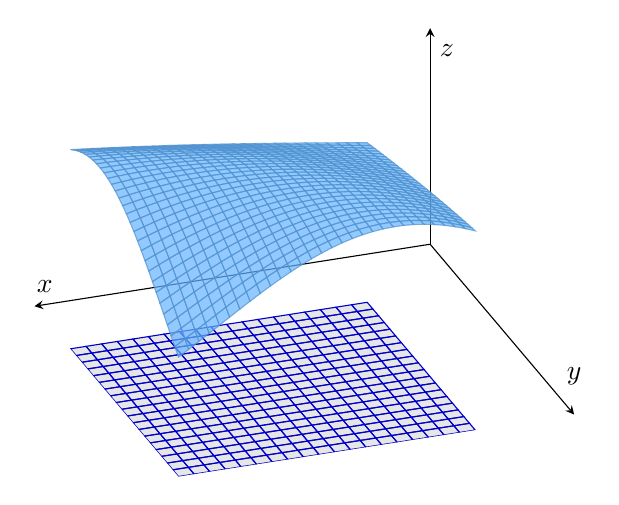
\begin{tikzpicture}
    \begin{axis}[
        view={160}{40},
        xmin=0, xmax=2,
        ymin=0, ymax=2,
        zmin=0, zmax=3,
        axis lines=center,
        ticks=none,
        xlabel={$x$}, ylabel={$y$}, zlabel={$z$},
        domain=0:2, y domain=0:2,
        samples=30, z buffer=sort
    ]
        % Región R (rectángulo base)
        \addplot3[
    surf,
    shader=faceted,
    draw=black, % dibuja las líneas de la malla
    fill=gray, fill opacity=0.2,
    domain=0.5:2, y domain=0.5:2,
    samples=20
] {0};

        % Superficie sobre región R (solo en R)
        \addplot3[
            surf, opacity=0.7, colormap={mycolor}{rgb255=(100,180,255) rgb255=(100,180,255)},
            domain=0.5:2, y domain=0.5:2,
        ] {sin(x*y*50)+2};
    \end{axis}
    \end{tikzpicture}
    \caption{Gráfica de \( f(x,y) \) sobre  \( R \)}
    \end{subfigure}
    \hfill
    % === Subfigura (b) ===
    \begin{subfigure}[b]{0.45\textwidth}
    \centering
    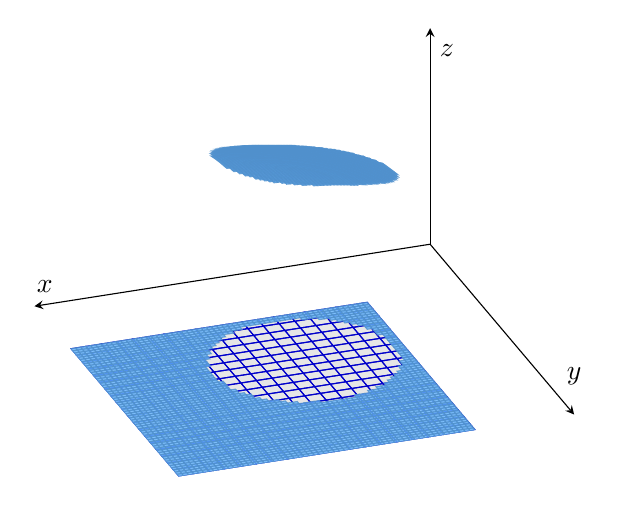
\begin{tikzpicture}
    \begin{axis}[
        view={160}{40},
        xmin=0, xmax=2,
        ymin=0, ymax=2,
        zmin=0, zmax=3,
        axis lines=center,
        ticks=none,
        xlabel={$x$}, ylabel={$y$}, zlabel={$z$},
        domain=0:2, y domain=0:2,
        samples=60, z buffer=sort
    ]

        % Superficie f(x,y) sobre toda R, con 0 fuera de D
        \addplot3[
            surf, opacity=0.8,
            domain=0.5:1.5, y domain=0.5:1.5,
            colormap={mycolor}{rgb255=(100,180,255) rgb255=(100,180,255)},
             restrict z to domain=2.1:10, % recorta para evitar planicies
    unbounded coords=jump,
        ]
        { ( (x-1)^2 + (y-1)^2 < 0.2 ) * sin(x*y*50)+2 };

         % Región R en gris claro
      \addplot3[
    surf,
    shader=faceted,
    draw=black, % dibuja las líneas de la malla
    fill=gray, fill opacity=0.2,
    domain=0.5:2, y domain=0.5:2,
    samples=20
] {0};
        
        \addplot3[
            surf, opacity=0.8,
            domain=0.5:2, y domain=0.5:2,
            colormap={mycolor}{rgb255=(100,180,255) rgb255=(100,180,255)},
             restrict z to domain=-0.1:0.1, % recorta para evitar planicies
    unbounded coords=jump,
        ]
        { ( (x-1)^2 + (y-1)^2 < 0.2 ) + 0 };

    \end{axis}
    \end{tikzpicture}
    \caption{Gráfica de \( f^*(x,y) \) sobre \( R \)}
    \end{subfigure}

    \caption{Integración doble sobre una región no rectangular \( D \subseteq R \)}
\end{figure}
\end{definition}

\begin{obs} 
La  definici\'on  (\ref{int_D})  es independiente  de la selecci\'on de $B$.
\end{obs}

\begin{propertie}
    Sean $f,\;g$ dos funciones integrables en una regi\'on $D\subset\Rn{2}$, entonces:
    \begin{enumerate}
        \item[i.] $\alpha f+\beta g$ es integrable en $D$, $\forall\;\alpha,\;\beta\in\R$ y, adem\'as,
        \[
            \iint_D \left(\alpha f+\beta g\right)dA=\alpha\iint_D f\:dA+\beta\iint_D g\:dA.
        \]
        \item[ii.] El producto $fg$ es integrable en $D$.
        \item[iii.] Si $|g(x,y)|\geq k>0\;\forall(x,y)\in D$, el cociente $f/g$ es integrable en $D$.
        \item[iv.] Si $f\geq 0$ en $D$, $\iint_D f\:dA\geq0$.
        \item[v.]Si $f\leq g$ en $D$, $\iint_D f\:dA\leq\iint_D g\:dA.$
        \item[vi.]Si $|f|$ es integrable en $D$, entonces 
        \[
            \left|\iint_D f\:dA\right|\leq\iint_D|f|\:dA.  
        \]    
        \item[vii.] Si $D=D_1\cup D_2$ donde $\;D_1\cap D_2$ es un conjunto de medida nula, entonces   $f$ es integrable sobre $D_1$ y sobre $D_2$ y, adem\'as,  
        \[
            \iint_D f\:dA=\iint_{D_1} f\:dA+\iint_{D_2}f\:dA.    
        \]
    \end{enumerate}
\end{propertie}

%-----------------------------------------------------------
\begin{definition}  Un conjunto  $D\subseteq\Rn{2}$ se llama elemental si puede ser descripto de alguna de las siguientes maneras. 
   
    \begin{enumerate}
    \item[i.]
    Existen funciones continuas $\phi_1,\;\phi_2:[a,b]\to\R$ tales que $D$ es el conjunto de puntos $(x,y)$ que satisfacen
    \[
        x\in[a,b], \qquad \phi_1(x)\leq y\leq\phi_2(x),  
    \]% no se pq no funciona \hfill para no usar \qquad
    donde $\phi_1(x) < \phi_2(x)\;\forall\;x\in[a,b].$  En tal  el conjunto $D$ se llama  \textit{elemental de tipo 1.} 
    \item[ii.]
    Si existen funciones continuas $\psi_1,\;\psi_2:[c,d]\to\R$ tales que $D$ es el conjunto de puntos $(x,y)$ que satisfacen
    \[
        y\in[c,d], \qquad \psi_1(y)\leq x\leq\psi_2(y),  
    \]
    donde $\psi_1(y) < \psi_2(y)\;\forall\;y\in[c,d].$ En tal  el conjunto $D$ se llama  \textit{elemental de tipo 2.} 
    \item[iii.]
    $D$ se llama conjunto elemental de \textit{tipo 3} si es \textit{tipo 1} y \textit{tipo 2} a la vez.
    
    
    
    
    \textcolor{red}{Dibujar los casos.}
    
    
    \end{enumerate}
\end{definition}

\begin{propertie} \label{col:fubini}
   
    \begin{enumerate}
        \item  Sea $f:D\to\R$ continua sobre  $D\subseteq\Rn{2}$  un conjunto de tipo 1, entonces
        \[
            \iint_D f=\int_a^b\left(\int_{\phi_1(x)}^{\phi_2(x)}f(x,y)\:dy\right)dx.  
        \]
        \item  Sea $f:D\to\R$ continua sobre  $D\subseteq\Rn{2}$  un conjunto de tipo 2, entonces
        % y las $\psi_i$ son continuas. 
        Entonces
        \[
            \iint_D f=\int_a^b\left(\int_{\psi_1(y)}^{\psi_2(y)}f(x,y)\:dx\right)dy.  
        \]
        \item  Sea $f:D\to\R$ continua sobre  $D\subseteq\Rn{2}$  un conjunto de tipo 3, entonces
        \[
            \iint_D f=\int_a^b\left(\int_{y=\phi_1(x)}^{y=\phi_2(x)}f(x,y)\:dy\right)dx=\int_a^b\left(\int_{x=\psi_1(y)}^{x=\psi_2(y)}f(x,y)\:dx\right)dy. 
        \]
    \end{enumerate}
\end{propertie}
\begin{example}
    Calcular $\iint_D f$, donde $f(x,y)=x^2y$, donde $D$ es la regi\'on del plano encerrado entre $y=x^3$, $y=x^2$, con $x\in[0,1]$. 

    \begin{center}
    \begin{tikzpicture}
        \begin{axis}[
            axis lines = middle,
            xmin = 0, xmax = 1.5,
            ymin = 0, ymax = 1.5,
            xlabel = {$x$},
            ylabel = {$y$},
            domain = 0:1.25,
            samples = 100,
            xtick={0.5,1},
            ytick={0.5,1},
            clip=false,
            ]
        
            % Define the curves
            \addplot[name path=A, blue, thick, domain=0:1.22] {x^2} node[pos=0.75, right] {$y=x^2$};
            \addplot[name path=B, red, thick, domain=0:1.15] {x^3} node[pos=0.3, below right] {$y=x^3$};
        
            % Fill the area between the curves
            \addplot[orange!50, fill opacity=0.5] fill between[of=A and B, soft clip={domain=0:1}];
        
            % Label the enclosed area as D
            \node at (axis cs:0.6,0.29) {$D$};
        
        \end{axis}
    \end{tikzpicture}
    \end{center}

    En este caso 
    \[
        D=\{(x,y)\in\Rn{2}:0\leq x\leq1;\;x^3\leq y\leq x^2\}.  
    \]
    Luego $D$ es de tipo 1. Notar que la \'unica manera de demostrar que un conjunto es elemental es dando su descripci\'on impl\'icita. Por el \autoref{col:fubini}
    \begin{gather*}
        \iint_D x^2y\:dA=\int_0^1\left(\int_{x^3}^{x^2}\:dy\right)dx=\int_0^1\left(x^2\frac{1}{2}y^2\Big\lvert_{x^3}^{x^2}\right)dx\\
        =\int_0^1\frac{1}{2}x^2\left((x^2)^2-(x^3)^2\right)=\int_0^1\frac{1}{2}x^6-\frac{1}{2}x^8\;dx\\=\frac{1}{14}x^7-\frac{1}{18}x^9\Big\lvert_0^1=\frac{1}{14}-\frac{1}{18}.
    \end{gather*}
\end{example}
\begin{definition} %cambie la palabra region --> conjunto
    Se define el \'area de un conjunto $D\subset\Rn{2}$, y se nota $\text{A}(D)$, a  
    \[
        \text{A}(D)=\iint_D1\:dA.
    \]
\end{definition}
\begin{theorem}
    \textbf{Teorema del valor medio para integrales dobles}. Sea $f:D\subseteq\Rn{2}\to\R$ continua y $D$ es un conjunto elemental. Entonces existe $(x_0,y_0)$ en $D$ tal que
    \[
        \int_D f(x,y)\:dA=f(x_0,y_0)\text{A}(D).
    \]
\end{theorem}


\textcolor{red}{Falta definir  $\boldsymbol{D}_\mathbf{F}$}


\begin{definition}
    Sea $\mathbf{F}:A\subseteq\Rn{n}\to\Rn{n}$ un campo $\mathcal{C}^1(A)$ y sea $\boldsymbol{D}_\mathbf{F}$ su matriz diferencial definida en $A$. Se define el \textbf{jacobiano}, o \textbf{determinante jacobiano}, y se lo nota $J_\mathbf{F}$ a 
    \[
        J_\mathbf{F}=\left|\text{det}(\boldsymbol{D}_\mathbf{F})\right|.
    \]
\end{definition}


\textcolor{red}{dos ejemplos  sencillos en n=2 y n=3}


\begin{theorem} % lo escribi como lo tenia en mis apuntes
    \textbf{Teorema del cambio de variables para integrales dobles}. Sea $f:D\subseteq\Rn{2}\to\Rn{2}$ un campo escalar integrable. Sea $\mathbf{T}:D^*\subseteq\Rn{2}\to D$ continua de clase $\mathcal{C}^1$ en $\interior{(D^*)}$, inyectiva en $\interior{(D^*)}$ y tal que $\mathbf{T}(D^*)=D$. Entonces
    \[
        \iint_D f\:dA=\iint_{D^*}(f\circ\mathbf{T})J_\mathbf{T}\:dA.
    \]
\end{theorem}
       
       \section{Integrales Triples}
           \input{capitulos/integrales_triples.tex}
        
        \section{Integrales de L\'inea}
            \begin{definition}
    Sea $\Gamma$ una curva simple en $\Rn{n}$ y sea $\boldsymbol{\sigma}:I\subseteq\R\to\Rn{n}$ una parametrizaci\'on regular $\mathcal{C}^1$ a trozos (\autoref{def:a-trozos}) de $\Gamma$. Se define la \emph{longitud de} $\Gamma$, y se nota  Long($\Gamma$), a 
    \[
        \text{Long}(\Gamma)=\sum_{i=1}^{m}\int_{I_i}\|\boldsymbol{\sigma}'(t)\|dt,    
    \]
    donde $\boldsymbol{\sigma}\lvert_{I_i}$ es de clase $\mathcal{C}^1$.
\end{definition}

\textcolor{red}{Ejemplos: puede ser la circunsferencia y un segmento.  Ilustrar}

\begin{definition}
    Sea $\boldsymbol{\sigma}:I=[a,b]\to\Rn{n}$ una trayectoria continua y de clase $\mathcal{C}^1(\interior{I})$ y sea $f$ un campo escalar tal que la funci\'on compuesta $f\circ\boldsymbol{\sigma}(t)$ sea continua en $I$. Se define la \emph{integral de trayectoria}, o \emph{integral de} $f$ \emph{a lo largo de la trayectoria} $\boldsymbol{\sigma}$, y se la nota $\int_{\boldsymbol{\sigma}}f\:ds$, a
    \[
        \int_{\boldsymbol{\sigma}}f\:ds=\int_a^b (f\circ\boldsymbol{\sigma})\|\boldsymbol{\sigma}'(t)\|\:dt.
    \]
\end{definition}

Si $\boldsymbol{\sigma}(t)$ es s\'olo $\mathcal{C}^1$ a trozos o $f\circ\boldsymbol{\sigma}(t)$ es continua a trozos, se define $\int_{\boldsymbol{\sigma}}f\:ds$ sobre una partici\'on de $[a,b]$, donde sobre cada intervalo de la partici\'on $(f\circ\boldsymbol{\sigma})\|\boldsymbol{\sigma}'(t)\|$ sea continua, y sumando las integrales sobre cada intervalo de la partici\'on. 

\begin{definition}
    Sea $\Gamma$ una curva simple en $\Rn{n}$ y sea $\boldsymbol{\sigma}:I\subseteq\R\to\Rn{n}$ una parametrizaci\'on regular de $\Gamma$.  Sea $f:A\subseteq\Rn{n}\to\R$ continua con $\Gamma \subset A$.  Se define la \emph{integral de l\'inea del campo $f$ sobre la curva} $\Gamma$, y se nota por $\int_{\Gamma}f\:ds$ a
    \[
        \int_{\Gamma}f\:ds=\sum_{i=1}^{m}\int_{I_i}f\circ\boldsymbol{\sigma}(t)\|\boldsymbol{\sigma}'(t)\|\:dt,  
    \]
    donde $\boldsymbol{\sigma}\lvert_{I_i}$ es de clase $\mathcal{C}^1$ e $I_i$ una partici\'on de $I$.

    \textcolor{red}{No es m\'as f\'acil decir que sigma es C1 a trozos y listo?}
\end{definition}

\begin{obs} La definici\'on anterior no depende de la parametrizaci\'on.
\end{obs} 

\textcolor{red}{Ejemplos.}

\begin{obs} 
 Sea $f:A\subseteq\Rn{2} \to\R$   tal que  $f(x,y)>0 \; \forall (x,y) \in A$ y   sea $\Gamma \subset A$ una curva simple en $\Rn{2}$.   La integral de l\'inea de $f$ sobre $\Gamma$  se puede interpretar geom\'etricamente como el ``\'area de la valla de base $\Gamma$ y altura $f$". 
\textcolor{red}{ilustracion de la aplicacion}
\end{obs}

\textcolor{red}{Ejemplo.}

\begin{definition}
    Sea $\mathbf{F}:A\subseteq\Rn{n}\to\Rn{n}$ un campo vectorial continuo sobre una curva simple orientada $\Gamma\subset A$. Sea $\boldsymbol{\sigma}:[a,b]\to A\subseteq\Rn{n}$ una parametrizaci\'on de $\Gamma$ que preserva su orientaci\'on. Se define la \emph{integral de} $\mathbf{F}$ \emph{sobre la curva simple} $\boldsymbol{\Gamma}$ como
    \[
        \int_{\Gamma}\mathbf{F}\cdot d\mathbf{s}=\int_{\boldsymbol{\sigma}}\mathbf{F}\cdot d\mathbf{s} 
    \]
\end{definition}

\begin{definition}
    Si $\Gamma$  es cerrada,  se suele notar a la integral como
    \[
        \oint_{\Gamma}\mathbf{F}\cdot d\mathbf{s},  
    \]  y se la llama integral de circulaci\'on de $\mathbf{F}$ sobre $\Gamma$.
\end{definition}

\begin{definition}
    Sean $\mathbf{F}:A\subseteq\Rn{n}\to\Rn{n}$ un campo vectorial y $\boldsymbol{\sigma}:[a,b]\to A\subseteq\Rn{n}$ una trayectorial $\mathcal{C}^1$ a trozos tales que $\mathbf{F}\circ\boldsymbol{\sigma}:[a,b]\to\Rn{n}$ es una funci\'on continua. Se define la \emph{integral de de l\'inea del campo vecorial} $\mathbf{F}$ \emph{a lo largo de la trayectoria} $\boldsymbol{\sigma}$ como
    \[
        \int_{\Gamma}\mathbf{F}\cdot d\mathbf{s}=\int_a^b\mathbf{F}\circ\boldsymbol{\sigma}(t)\cdot\boldsymbol{\sigma}'(t)\:dt. 
    \]
\end{definition}

Se usa la notaci\'on $\int_{\boldsymbol{\sigma}}\mathbf{F}\cdot d\mathbf{s}=\int_{\boldsymbol{\sigma}}\mathbf{F}\cdot\hat{\mathbf{t}}\:ds$,  donde $\hat{\mathbf{t}}$ es versor tangencial a la curva  $\Gamma = Img(\boldsymbol{\sigma}).$

        
        \section{Integrales de Superficie}
            \begin{definition} Sea  $\boldsymbol{\Sigma}:D \subseteq\Rn{2} \to\Rn{3}$ continua y de clase $\mathcal{C}^1(\interior{D})$.  Al conjunto  $S = \text{Img}(\Sigma)$ se lo llama  \emph{superficie}   parametrizada por  $\boldsymbol{\Sigma}$  y   
   a  $\boldsymbol{\Sigma}$  una \emph{parametrizaci\'on} de $S$.
\end{definition}

\begin{definition}
    Sea $\boldsymbol{\Sigma}:D\subseteq\Rn{2} \to\Rn{3}$ una parametrizaci\'on de $S$ y sea $(u_0, v_0) \in \interior{D}$.   $\boldsymbol{\Sigma}$ se llama  \emph{parametrizaci\'on regular de $S$} en  $(u_0, v_0)$ si
    \[
        \boldsymbol{\Sigma}_u(u_0,v_0)\times\boldsymbol{\Sigma}(u_0,v_0)\neq \boldsymbol{0}.
    \]
    En tal caso, $S$ se llama superficie regular en $\boldsymbol{\Sigma}(u_0,v_0)$ . Si $S$   admite una parametrizaci\'on regular en todo el interior de su dominio diremos que  $S$ es una superficie regular.
\end{definition}

\begin{definition}
    Sea $S\subseteq\Rn{3}$. Se define a $S$ como \emph{orientable} si existe un campo vectorial $\boldsymbol{\eta}:S\to\Rn{3}$, continuo talque $\boldsymbol{\eta}(\mathbf{p})$ es ortogonal a $S$ en $\mathbf{p}$ y $\norm{\boldsymbol{\eta}(\mathbf{p})}=1\;\forall \mathbf{p}\in S$. Al campo $\boldsymbol{\eta}$ se lo llama \emph{orientaci\'on} de $S$. De no existir tal $\boldsymbol{\eta}$ diremos que la superficie se \emph{no orientable}.
\end{definition}


\begin{obs} Notar que para cualquier campo escalar $f:\Rn{2}\to\R$, su gr\'afica Graf$(f)$ es una superficie con parametrización $\boldsymbol{\Sigma}(x,y)=(x,y,f(x,y))$.
\end{obs}


\begin{example} Sea $f(x,y) = x^2-y^2$. Por la observaci\'on anterior sabemos que la gr\'afica de $f$ es una superficie y existe una parametrización $\boldsymbol{\Sigma}(x,y)=(x,y,x^2-y^2)$. La gr\'afica de $f$ constituye a una superficie orientable. Por otro lado, una superficie no orientable es el de una cinta de Möebius. Ambas superficies se ilustran a continuaci\'on.
\input{figs/moebius.tex}
\end{example}

\begin{obs}
    Sea $S$ una superficie orientable. Entonces $S$ admite dos orientaciones posibles: $\boldsymbol{\eta}$ y $-\boldsymbol{\eta}$.
\end{obs}

\begin{definition}\label{def:preseva}
    Sea $S\subseteq\Rn{3}$ una superficie orientada por $\boldsymbol{\eta}$. Sea $\boldsymbol{\Sigma}:D\subseteq\Rn{2}\to S$ una parametrizaci\'on continua de clase $\mathcal{C}^1$ y regular de $S$.
    \begin{itemize}
        \item Si \[
            \frac{\boldsymbol{\Sigma}_u\times\boldsymbol{\Sigma}_v}{\norm{\boldsymbol{\Sigma}_u\times\boldsymbol{\Sigma}_v}}(u,v)=\boldsymbol{\eta}\left(\boldsymbol{\Sigma}(u,v)\right),
        \]  
        decimos que $\boldsymbol{\Sigma}$ \emph{preserva} la orientaci\'on de $S$.
        \item Si \[
            \frac{\boldsymbol{\Sigma}_u\times\boldsymbol{\Sigma}_v}{\norm{\boldsymbol{\Sigma}_u\times\boldsymbol{\Sigma}_v}}(u,v)=-\boldsymbol{\eta}\left(\boldsymbol{\Sigma}(u,v)\right),
        \]
        decimos que $\boldsymbol{\Sigma}$ \emph{invierte} la orientaci\'on de $S$.  
    \end{itemize}
    Para ambos casos, decimos que $\boldsymbol{\Sigma}$ \emph{induce} una orientaci\'on sobre $S$.
\end{definition}

 \textcolor{red}{OJO. Falta todo lo de campos escalares.}

\begin{definition}
    Sea $S\subseteq\Rn{3}$ una superficie orientada por $\boldsymbol{\eta}$. Sea $\mathbf{F}:A \subset \to\Rn{3}$ con $S\subset A$ un campo continuo. Se define la integral de superficie de $\mathbf{F}$ sobre $S$, y se nota  $\iint_S\mathbf{F}\cdot \mathbf{S},$ a
    \[
        \iint_S \mathbf{F}\;d\mathbf{S}=\iint_S (\mathbf{F}\cdot\boldsymbol{\eta}) \;dS.
    \]
\end{definition}

\begin{obs}   Sean $S\subseteq\Rn{3}$ una superficie orientada por $\boldsymbol{\eta}$ y  sea  $\boldsymbol{\Sigma}:D\subseteq\Rn{2}\to S\subseteq\Rn{3}$ una parametrizaci\'on de $S$ tal que preserve su orientaci\'on, entonces 
 $$ \iint_S \mathbf{F}\cdot d\mathbf{S} = \iint_D \mathbf{F}\circ\boldsymbol{\Sigma}\cdot\left(\boldsymbol{\Sigma}_u\times\boldsymbol{\Sigma}_v\right)dudv.$$
\end{obs}
Veamos que esto efectivamente es as\'i.  Sabemos que, por la \autoref{def:preseva},
\[
    \frac{\boldsymbol{\Sigma}_u\times\boldsymbol{\Sigma}_v}{\norm{\boldsymbol{\Sigma}_u\times\boldsymbol{\Sigma}_v}}(u,v)=\boldsymbol{\eta}\left(\boldsymbol{\Sigma}(u,v)\right).
\]
Entonces,
\begin{align*}
    \iint_S \mathbf{F}\cdot d\mathbf{S}&=\iint_S \mathbf{F}\cdot\boldsymbol{\eta}\;dS=\iint_D (\mathbf{F}\cdot\boldsymbol{\eta})\circ\boldsymbol{\Sigma}\:\norm{\boldsymbol{\Sigma}_u\times\boldsymbol{\Sigma}_v}\;dudv\\[.2cm]
    &=\iint_D (\mathbf{F}\circ\boldsymbol{\Sigma})\cdot(\boldsymbol{\eta}\circ\boldsymbol{\Sigma})\norm{\boldsymbol{\Sigma}_u\times\boldsymbol{\Sigma}_v}\;dudv=\iint_D \mathbf{F}\circ\boldsymbol{\Sigma}\cdot\left(\boldsymbol{\Sigma}_u\times\boldsymbol{\Sigma}_v\right)dudv,
\end{align*} concluyendo lo que quer\'iamos ver.

\begin{obs}
    Sea $S$ una superficie con orientaci\'on $\boldsymbol{\eta}$. Sea $\boldsymbol{\Sigma}:D\subseteq\Rn{2}\to S\subseteq\Rn{3}$, una parametrizaci\'on de $S$ que invierte la orientaci\'on. Entonces
    \[
        \iint_S \mathbf{F}\cdot d\mathbf{S} = \iint_S \mathbf{F}\cdot\eta\;dS=-\iint_D \mathbf{F}\circ\boldsymbol{\Sigma}\cdot(\boldsymbol{\Sigma}_u\times\boldsymbol{\Sigma}_v)\:dudv.
    \]
\end{obs}


      
        \section{Campos Conservativos}
            \begin{theorem} \label{thm:t1}
    Sean $A\subseteq\Rn{n}$ un conjuto abierto y conexo y  $f:A\subseteq\Rn{n}\to\R$ un campo de clase $\mathcal{C}^1(\interior{A})$. Si $\boldsymbol{\sigma}:[a,b]\to A\subseteq\Rn{n}$ es una trayectoria continua,  entonces
    \[
       \int_{\boldsymbol{\sigma}}\grad f\cdot d\mathbf{s}=f(\boldsymbol{\sigma}(b))-f(\boldsymbol{\sigma}(a)).
    \]    

    \textit{Demostración.}
    Al aplicar la regla de la cadena a la función compuesta
    \begin{equation*}
        F:t \rightarrow f(\boldsymbol{\sigma}(t))
    \end{equation*}
    se obtiene
    \begin{equation*}
        F'(t)=(f\circ\boldsymbol{\sigma})'(t)=\grad{f(\boldsymbol{\sigma})}\cdot\boldsymbol{\sigma}'(t)
    \end{equation*}
    La función F es una función con valores reales de la variable $t$ y, por lo tanto, por el teorema fundamental
    del cálculo de una variable:
    \begin{equation*}
        \int_{a}^{b}F'(t)dt=F(b)-F(a)=f(\boldsymbol{\sigma}(b))-f(\boldsymbol{\sigma}(a)).
    \end{equation*}
    Por consiguiente,
    \begin{align*}
        \int_{\boldsymbol{\sigma}}\grad f\cdot d\mathbf{s}&=\int_{a}^{b}\grad{f(\boldsymbol{\sigma}(t))}\cdot\boldsymbol{\sigma}'(t)dt\\
        &=\int_{a}^{b}F'(t)dt=F(b)-F(a)\\
        &=f(\boldsymbol{\sigma}(b))-f(\boldsymbol{\sigma}(a)).
    \end{align*}
\end{theorem}



\begin{corollary}\label{tmh:c1}
    Sean $A\subseteq\Rn{n}$ un conjuto abierto y conexo y  $f:A\subseteq\Rn{n}\to\R$ un campo de clase $\mathcal{C}^1(\interior{A})$.  Si  $\boldsymbol{\sigma}_1:[a_1,b_1]\to A_1\subseteq\Rn{n}$ y $\boldsymbol{\sigma}_2:[a_2,b_2]\to A_2\subseteq\Rn{n}$ son dos trayectorias continuas  tales que $\boldsymbol{\sigma}_1(a_1)=\boldsymbol{\sigma}_2(a_2)\;\land\;\boldsymbol{\sigma}_1(b_1)=\boldsymbol{\sigma}_2(b_2)$, entonces
    \[
    \int_{\boldsymbol{\sigma}_1}\grad f\cdot d\mathbf{s}=\int_{\boldsymbol{\sigma}_2}\grad f\cdot d\mathbf{s}.
    \]
    
 Es decir,  $\int_{\boldsymbol{\sigma}}\grad f\cdot d\mathbf{s}$  s\'olo depende de los puntos inicial y final de la trayectoria.

\textit{Demostración.} 
Usando el Teorema \ref{thm:t1}, se tiene que
\begin{align*}
    \int_{\boldsymbol{\sigma}_1}\grad f\cdot d\mathbf{s}&=f(\boldsymbol{\sigma}_1(b_1))-f(\boldsymbol{\sigma}_1(a_1))\\
    \int_{\boldsymbol{\sigma}_2}\grad f\cdot d\mathbf{s}&=f(\boldsymbol{\sigma}_2(b_2))-f(\boldsymbol{\sigma}_2(a_2)).
\end{align*}
Así, con $\boldsymbol{\sigma}_1(a_1)=\boldsymbol{\sigma}_2(a_2)\;\land\;\boldsymbol{\sigma}_1(b_1)=\boldsymbol{\sigma}_2(b_2)$,
\begin{equation*}
    f(\boldsymbol{\sigma}_1(a_1))=f(\boldsymbol{\sigma}_2(a_2))\;\land\;f(\boldsymbol{\sigma}_1(b_1))=f(\boldsymbol{\sigma}_2(b_2))
\end{equation*}
Luego,
\begin{equation*}
    f(\boldsymbol{\sigma}_1(b_1))-f(\boldsymbol{\sigma}_1(a_1))=f(\boldsymbol{\sigma}_2(b_2))-f(\boldsymbol{\sigma}_2(a_2))
\end{equation*}
Por lo tanto, se demuestra que:
\begin{equation*}
    \int_{\boldsymbol{\sigma}_1}\grad f\cdot d\mathbf{s}=\int_{\boldsymbol{\sigma}_2}\grad f\cdot d\mathbf{s}.
\end{equation*}
\end{corollary}


\begin{corollary}\label{tmh:c2}
    Sean $A\subseteq\Rn{n}$ abierto y conexo y $f:A\subseteq\Rn{n}\to\R$ de clase $\mathcal{C}^1$. Si $\mathbf{F}:A\subseteq\Rn{n}\to\Rn{n}$ es un campo vectorial para el cual $\exists f:A\subseteq\Rn{n}\to\R$ clase $\mathcal{C}^1$ tal que 
    $$\grad f(\mathbf{x})=\mathbf{F}(\mathbf{x})\quad\forall\:\mathbf{x}\in A,$$
    entonces para todo par de curvas $C_1$ y $C_2$ en $A$, con los mismos extremos y misma orientaci\'on,
    \[
    \int_{C_1}\mathbf{F}\cdot d\mathbf{s}=\int_{C_2}\mathbf{F}\cdot d\mathbf{s}. 
    \]
    Dada esta igualdad, se dice que la integral de línea de un campo conservativo tiene \textit{independencia del camino}.

    \textit{Demostración.} 
    Sean $C_1$ y $C_2$ parametrizadas por las trayectorias $\boldsymbol{\sigma}_1:[a_1,b_1]\to C_1$ y $\boldsymbol{\sigma}_2:[a_2,b_2]\to C_2$, con $\grad f(\mathbf{x})=\mathbf{F}(\mathbf{x})$:
    \begin{align*}
        \int_{C_1}\mathbf{F}\cdot d\mathbf{s}&=\int_{\boldsymbol{\sigma}_1}\grad f\cdot d\mathbf{s}\\
        \int_{C_2}\mathbf{F}\cdot d\mathbf{s}&=\int_{\boldsymbol{\sigma}_2}\grad f\cdot d\mathbf{s}
    \end{align*}
    Además, como $C_1$ y $C_2$ comparten extremos, se da que $\boldsymbol{\sigma}_1(a_1)=\boldsymbol{\sigma}_2(a_2)\;\land\;\boldsymbol{\sigma}_1(b_1)=\boldsymbol{\sigma}_2(b_2)$.
    Por lo tanto, según el Corolario \ref{tmh:c1}:
    \begin{align*}
        \int_{\boldsymbol{\sigma}_1}\grad f\cdot d\mathbf{s}&=\int_{\boldsymbol{\sigma}_2}\grad f\cdot d\mathbf{s}\\
        \therefore \int_{C_1}\mathbf{F}\cdot d\mathbf{s}&=\int_{C_2}\mathbf{F}\cdot d\mathbf{s}
    \end{align*}
\end{corollary}

\begin{corollary}\label{tmh:c3}
    Sean $A\subseteq\Rn{n}$ abierto y conexo y $f:A\subseteq\Rn{n}\to\R$ de clase $\mathcal{C}^1$. Si $\mathbf{F}=\grad f$, entonces
    $$\oint_C\mathbf{F}\cdot d\mathbf{s}=0,$$
    para toda curva $C$ simple cerrada contenida en $A$.

    \textit{Demostración.} 
    Sea $C$ parametrizada por la trayectoria continua $\boldsymbol{\sigma}:[a,b]\to C$, y $\mathbf{F}=\grad f$:
    \begin{equation*}
        \oint_C\mathbf{F}\cdot d\mathbf{s}=\int_{\sigma}\grad f\cdot d\mathbf{s}
    \end{equation*}
    Cumpliéndose las hipótesis del Teorema \ref{thm:t1},
    \begin{equation*}
        \int_{\sigma}\grad f\cdot d\mathbf{s}=f(\boldsymbol{\sigma}(b))-f(\boldsymbol{\sigma}(a))
    \end{equation*}
    Ahora, como $C$ es cerrada, $\boldsymbol{\sigma}(a)=\boldsymbol{\sigma}(a)$, entonces $f(\boldsymbol{\sigma}(b))=f(\boldsymbol{\sigma}(a))$, y,
    \begin{align*}
        \int_{\sigma}\grad f\cdot d\mathbf{s}&=0\\
         \therefore \oint_C\mathbf{F}\cdot d\mathbf{s}&=0
    \end{align*}

\end{corollary}

\textit{Notación:} $\int_{\mathbf{x}_0}^{\mathbf{x}}\mathbf{F}\cdot d\mathbf{s}$ indica la integral de camino de el campo $\mathbf{F}$ sobre la recta que une los puntos $\mathbf{x}_0$
    y $\mathbf{x}$, orientada desde el primero hacia el segundo.

\begin{theorem}\label{tmh:t2}
   Sea  $\mathbf{F}:A\subseteq\Rn{n} \to \Rn{n}$ continuo con  $A$ abierto y conexo. Si  $\int_C \mathbf{F}\cdot d\mathbf{s}$ es independiente del camino en $A$  entonces el campo
    $$f:A\subseteq\Rn{n}\to\R\: | \:f(\mathbf{x})=\int_{\mathbf{x}_0}^{\mathbf{x}}\mathbf{F}\cdot d\mathbf{s},  \mbox{ con }  \mathbf{x}_0\in A, $$
    cumple que: 
    \begin{enumerate}
        \item $f$ es $\mathcal{C}^1$.
        \item $\grad f(\mathbf{x})=\mathbf{F}(\mathbf{x})\quad\forall\:\mathbf{x}\in A.$
    \end{enumerate}
\end{theorem}

\begin{theorem}
    Sean $A\subseteq\Rn{n}$ abierto y conexo, $\mathbf{F}:A\subseteq\Rn{n}\to\R$ continuo. Las siguientes proposiciones sobre $\mathbf{F}$ son equivalentes:
    \begin{enumerate}
        \item $\exists f:A\subseteq\Rn{n}\to\R$ de clase $\mathcal{C}^1$ tal que $\mathbf{F}(\mathbf{x})=\grad f(\mathbf{x}),\;\forall\mathbf{x}\in A.$ 
        \item La integral de $\mathbf{F}$ es independiente del camino en $A$.
        \item $\oint_C\mathbf{F}\cdot d\mathbf{s}=0$ para toda curva cerrada simple $C$ en $A$.
    \end{enumerate}

    \textit{Demostración.}
    Se deben demostrar las implicaciones de a pares. 
    
    \begin{equation}
        \mathbb{F}(\mathbf{x})=\grad f(\mathbf{x}) \then \int_{C_1}\mathbf{F}\cdot d\mathbf{s}=\int_{C_2}\mathbf{F}\cdot d\mathbf{s}.
        \label{eq:CampoCons1}
    \end{equation}
    Con $C_1$ y $C_2$ de iguales extremos. En tanto $\mathbb{F}(\mathbf{x})=\grad f(\mathbf{x})$, y $\boldsymbol{\sigma}_1:[a_1,b_1]\to C_1$ una parametrización continua de $C_1$, según el Teorema \ref{thm:t1},
    \begin{equation*}
        \int_{C_1}\mathbf{F}\cdot d\mathbf{s}=\int_{\boldsymbol{\sigma}_1}\grad f(\mathbf{x})\cdot d\mathbf{s}=f(\boldsymbol{\sigma}_1(b_1))-f(\boldsymbol{\sigma}_1(a_1))
    \end{equation*}
    Esto se cumple análogamente para $C_2$ con parametrización $\boldsymbol{\sigma}_2:[a_2,b_2]\to C_2$. Como $C_1$ y $C_2$ comparten extremos
    \begin{align*}
        \boldsymbol{\sigma}_1(a_1)=\boldsymbol{\sigma}_2(a_2) \quad &\land \quad \boldsymbol{\sigma}_1(b_1)=\boldsymbol{\sigma}_2(b_2)\\
        f(\boldsymbol{\sigma}_1(a_1))=f(\boldsymbol{\sigma}_2(a_2)) &\quad \land \quad f(\boldsymbol{\sigma}_1(b_1))=f(\boldsymbol{\sigma}_2(b_2))\\
        \then f(\boldsymbol{\sigma}_1(b_1))-f(\boldsymbol{\sigma}_1(a_1))&=f(\boldsymbol{\sigma}_2(b_2))-f(\boldsymbol{\sigma}_2(a_2))\\
        \therefore \int_{C_1}\mathbf{F}\cdot d\mathbf{s}&=\int_{C_2}\mathbf{F}\cdot d\mathbf{s}
    \end{align*}

    \begin{equation}
        \int_{C_1}\mathbf{F}\cdot d\mathbf{s}=\int_{C_2}\mathbf{F}\cdot d\mathbf{s} \then \mathbb{F}(\mathbf{x})=\grad f(\mathbf{x}).
        \label{eq:CampoCons2}
    \end{equation}
    Esta proposición es verdadera por el Teorema \ref{tmh:t2}.

    A partir de las ecuaciones (\ref{eq:CampoCons1}) y (\ref{eq:CampoCons2}) se demostró que
    \begin{equation}
        \mathbb{F}(\mathbf{x})=\grad f(\mathbf{x}) \Leftrightarrow \int_{C_1}\mathbf{F}\cdot d\mathbf{s}=\int_{C_2}\mathbf{F}\cdot d\mathbf{s}.
        \label{eq:CampoCons1y2}
    \end{equation}

    \begin{equation}
        \mathbb{F}(\mathbf{x})=\grad f(\mathbf{x}) \then \oint_C\mathbf{F}\cdot d\mathbf{s}=0
        \label{eq:CampoCons3}
    \end{equation}
    Esta proposición es verdadera por el Corolario \ref{tmh:c3}.

    \begin{equation}
        \oint_C\mathbf{F}\cdot d\mathbf{s}=0 \then \int_{C_1}\mathbf{F}\cdot d\mathbf{s}=\int_{C_2}\mathbf{F}\cdot d\mathbf{s}
        \label{eq:CampoCons4}
    \end{equation}
    Para la demostración pensemos en dos curvas con iguales extremos, $C_1$ y $C_2$.
    \begin{figure}[H]
        \begin{center}
            \begin{tikzpicture}[scale=2, >=stealth]

                % Puntos A y B
                \coordinate (A) at (0,0);
                \coordinate (B) at (3,0);

                % Primer camino: curva hacia arriba (gamma_1)
                \draw[thick, blue, ->, decoration={markings, mark=at position 0.5 with {\arrow{>}}},
                    postaction={decorate}] 
                    (A) .. controls (1,1.5) and (2,1.5) .. (B) node[midway, above] {$C_1$};

                % Segundo camino: curva hacia abajo (gamma_2)
                \draw[thick, red, ->, decoration={markings, mark=at position 0.5 with {\arrow{>}}},
                    postaction={decorate}] 
                    (B) .. controls (1,-1.5) and (2,-1.5) .. (A) node[midway, below] {$C_2$};

                % Nombres de los puntos
                \filldraw (A) circle(0.03) node[below left] {$A$};
                \filldraw (B) circle(0.03) node[below right] {$B$};

            \end{tikzpicture}
            \caption{Curvas $C_1$ y $C_2$.}
        \end{center}
    \end{figure}
    Luego, se puede pensar la curva $C=C_1\cup\overline{C_2}$ con $\overline{C_2}$ la curva $C_2$ en sentido opuesto. Así:
    \begin{align*}
        \oint_C\mathbf{F}\cdot d\mathbf{s}&=\int_{C_1}\mathbf{F}\cdot d\mathbf{s}+\int_{\overline{C_2}}\mathbf{F}\cdot d\mathbf{s}\\
        0&=\int_{C_1}\mathbf{F}\cdot d\mathbf{s}-\int_{C_2}\mathbf{F}\cdot d\mathbf{s}\\
        \therefore \int_{C_1}\mathbf{F}\cdot d\mathbf{s}&=\int_{C_2}\mathbf{F}\cdot d\mathbf{s}
    \end{align*}
   
    A partir de haber demostrado (\ref{eq:CampoCons3}), (\ref{eq:CampoCons4}) y (\ref{eq:CampoCons1y2}) se construye lógicamente las equivalencias de este teorema.
\end{theorem}


       
        \section{Teoremas Integrales}
            \input{capitulos/teo_integrales.tex}


%===================================================
%               EJERCICIOS RESUELTOS
%===================================================
    \chapter{Primeros parciales resueltos}
        \section{Fecha 29 de septiembre de 2023}
            \input{capitulos/1p_29_09_2023}

        \newpage
        \section{Fecha 25 de abril de 2023}
            \input{capitulos/1p_25_04_2023}





            \newpage
        \section{Fecha 23 de septiembre de 2023}
            
%----------------------------------------------------------------
\begin{question}
    Considere la función

     \[
        f(x,y) =
        \begin{dcases}
            \frac{e^{x^{2}+y^{2}}-1}{\sqrt{x^{2}+y^{2}}} & \textnormal{si}\ (x,y) \neq (0,0) \\
            0                         & \textnormal{si}\ (x,y) = (0,0)
        \end{dcases}
    \]

    \begin{enumerate}
        \item Analizar la continuidad de $f$ en el origen
        \item Analizar la diferenciabilidad de $f$ en el origen.
        \item Analizar la existencia de las derivadas direccionales de $f$ en el origen.\\
    \end{enumerate}
\end{question}

%---------------------------------------------------------------------
\begin{question}
    Sean $f:\Rn{2}\to\R$ diferenciable, $g(x,y)=(xy^2,x^2-2y)$ y $h=f\circ g$. Sabiendo que $h(1,-1) = 2$ y que $\grad h(1,-1)=(2,-4)$, halle el plano tangente al gráfico de $f$ en el punto $(1,3,f(1,3))$.
\end{question}
%------------------------------------------------
\begin{question}
    Sean $f$ y $g$ dos campos escalares de clase $\mathcal{C}^2$ tales que $f(1,2)=g(x,y)$, $\grad f(1,-1)=\grad g(2,-4)$ y $H_f(1,2)=H_g(1,2)$, calcular 
    
\[
        \lim_{(x,y)\to(1,2)} \
        \frac{f^2(x,y)-g^2(x,y)}{x^2+y^2-2x-4y+5}
    \]
\end{question}
%------------------------------------------------------------------
\begin{question}
    Hallar analíticamente los puntos más lejanos y más cercanos al origen del elipsoide dado por la ecuación {\large$\frac{x^2}{64}+\frac{y^2}{36}+\frac{z^2}{25}-1=0$}
\end{question}
%---------------------------------------------------------------------
\newpage

\begin{solution}
    En primer lugar analizamos la continuidad, como $f$ es una función partida, queremos demostrar que $f$ es continua en (0,0) si:  $\lim_{(x,y)\to(0,0)} \ f(x,y) = f(0,0)=0$

 
Utilizando el límite notable conocido:  $ \lim_{t\to 0} \
        (\frac{e^{t}-1}{t})=1$ , sabemos que 
\[
        \lim_{t\to 0} \
        \frac{e^{t}-1}{\sqrt{t}}=0 
    \]
    Pues, multiplicando arriba y abajo por $\sqrt{t}$, sabiendo que $t\neq 0$, tenemos que
    \[
        \lim_{t\to 0} \
        (\frac{e^{t}-1}{\sqrt{t}})(\frac{\sqrt{t}}{\sqrt{t}}) =\lim_{t\to 0} \
        (\frac{e^{t}-1}{t})\sqrt{t}=0
    \]
    Llamamos  $t(x,y)=x^{2}+y^{2}$ y sabemos que 
   \[
        \lim_{(x,y)\to(0,0)} t(x,y)=0
    \]
    Definimos $g(z)=\frac{e^{z}-1}{\sqrt{z}}=0 $ y realizando la composición $f(x,y)=g\circ t(x,y) \hspace{0.25cm}\forall (x,y)\in \mathbb{R}^ 2 -(0,0)$ tenemos que
\[
        \lim_{(x,y)\to (0,0)} \
        g\circ t(x,y)=\lim_{(x,y)\to (0,0)} \
        g(t(x,y))=\lim_{t\to 0} \
        \frac{e^{t}-1}{\sqrt{t}}=0 
    \]
    
   $\therefore f$ es continua en $(0,0)$
   

    Para analizar la diferenciabilidad de $f$ en el (0,0) en primer lugar vamos a evaluar la existencia de las derivadas direccionales, siendo $\vec{u}=(u_1,u_2)$ con $|\vec{u}|=1$
    
  \[
\displaystyle\frac{\partial f}{\partial \vec{u}}(0,0)=  \lim_{h\to 0} \
        \frac{f((0,0)+h\vec{u})-f(0,0)}{h}=  \lim_{h\to 0} \
        \frac{f(hu_1,hu_2)-f(0,0)}{h}= \lim_{h\to 0} \
        \frac{e^{h^2u_1^2+h^2u_2^2}-1}{h\sqrt{h^2u_1^2+h^2u_2^2}} 
 \]
 
  Sabemos que 
         \[
       |\vec{u}|=1   \iff \sqrt{u_1^2+u_2^2}=1  \iff u_1^2+u_2^2 =1
        \]
         
          Por lo cuál
 \[
\displaystyle\frac{\partial f}{\partial \vec{u}}(0,0)=   \lim_{h\to 0} \
        \frac{e^{h^2}-1}{h|h|} = \lim_{h\to 0} \
        \frac{e^{h^2}-1}{h^2}\frac{h}{|h|}
 \]

Tomando límites laterales
\[
\lim_{h\to 0^+} \
        \frac{e^{h^2}-1}{h^2}\frac{h}{|h|}=1
        \]
\[   
    \lim_{h\to 0^-} \
    \frac{e^{h^2}-1}{h^2}\frac{h}{|h|}=-1 
\]
 Como los límites laterales son distintos, entonces podemos afirmar que $\nexists   $ 
  $ \displaystyle\frac{\partial f}{\partial \vec{u}}(0,0)    $       $     \forall \vec{u} /|\vec{u}|=1$ , al no existir las derivadas direccionales de $f$ en $(0,0)$, las parciales tampoco.

  $\therefore $  $f$ no es diferenciable en $(0,0)$
\end{solution}
\newpage
\begin{solution}

    Como   $f:\Rn{2}\to\R$ es diferenciable en todo su dominio por ser composición de funciones diferenciables,  la ecuaci\'on de su plano tangente en el punto $(1,3)$ est\'a dada por
    \begin{equation}
        z= f(1,3) + \grad f(1,3) (x-1,y-3),  \label{eq:zNabla}
    \end{equation}   luego ser\'a  suficente con encontar $ f(1,3)$ y $\grad f(1,3).$

    Por un lado,      $h(1,-1)= f\circ g (1,-1) =  f(1,3)=2$  y por otro lado,  como $f$ y $g$ son ambas diferenciables,  por la regla de la cadena,  tenemos que
    \begin{equation}
        \grad h(1,-1)=\grad (f\circ g)(1,-1)=\grad f(g(1,-1)) \:\boldsymbol{D}_g(1,-1) = \grad f (1,3) \:\boldsymbol{D}_g(1,-1),  \label{eq:hNabla}
    \end{equation}    donde $\boldsymbol{D}_g$ es la matriz diferencial o  jacobiana de $g$.

    \noindent  Hallemos $\boldsymbol{D}_g$
    \begin{align*}
        \boldsymbol{D}_g(1,-1) & =
        \left(\begin{array}{cc}
                      \displaystyle\partialx (xy^2)            & \displaystyle\partialy (xy^2)           \\[10pt]
                      \displaystyle\partialx  (x^2 -2y) & \displaystyle\partialy (x^2 -2y)
                  \end{array}\right)\left.\rule{0pt}{1.1cm}\right\rvert_{(1,-1)}             \\[2pt]
                              & =\left(\begin{array}{cc}
                                               \displaystyle y^2                 & \displaystyle 2xy              \\[5pt]
                                               \displaystyle   2x & \displaystyle -2
                                           \end{array}\right)\left.\rule{0pt}{0.7cm}\right\rvert_{(1,-1)} \\[2pt]
                              & =\left(\begin{array}{cc}
                                               1    & -2    \\
                                               2 & -2
                                           \end{array}\right)
    \end{align*}
    Luego, reemplazando en  a   \eqref{eq:hNabla}
    \[
        \grad h(1,-1) = \grad f(1,3)\left(\begin{array}{cc}
                1   & -2    \\
                2 & -2
            \end{array}\right) = \left(f_x(1,3) + 2f_y(1,3),\;-2f_x(1,3)-2f_y(1,3)\right)
    \]

    y con la información de la consigna, se despejan
    \[\begin{cases}
            \;f_x(1,3) + 2f_y(1,3)=2 \\[5pt]
            \;-2f_x(1,3)- 2f_y(1,3)=-4
        \end{cases}
        \iff
        \begin{cases}
            \;f_x(1,3)=2 \\[5pt]
            \;f_y(1,3)=0
        \end{cases}
    \]
    $\therefore\quad\grad f(1,3)=(2,0)$.

       Reemplazando en \eqref{eq:zNabla}
      \[
        z= 2 + (2,0)(x-1,y-3)
    \]


        Despejando, la ecuación del plano tangente al grafico de $f$ en el punto $(1,3,f(1,3))$ es
          \[
         z -2x = 0
    \]
 
\newpage
\end{solution}

\begin{solution}
   En primer lugar, reescribimos el límite pedido 
   \[
        \lim_{(x,y)\to(1,2)} \
        \frac{(f-g)_{(x,y)}(f+g)_{(x,y) }}{|(x-1,y-2)|^2}
    \]
    Dado que $f$  y $g$ son dos campos escalares de clase  $\mathcal{C}^2(\mathbb{R}^2)$,  se define  el polinomio de Taylor de primer orden centrado en $(1,2)$ de ambas funciones, que noteremos por $P_2[f,(1,2)]$ , $P_2[g,(1,2)]$ como,
    \begin{equation}
        P_2[f,(1,2)](x,y)=f(1,2)+\grad f(1,2)\cdot(x-1,y-2)+ \frac{1}{2}(x,y)\boldsymbol{H}_f(c_1,c_2)\begin{pmatrix}x-1\\y-2\end{pmatrix}, \label{eq:polTay2}
    \end{equation}
    \begin{equation}
        P_2[g,(1,2)](x,y)=f(1,2)+\grad f(1,2)\cdot(x-1,y-2)+ \frac{1}{2}(x,y)\boldsymbol{H}_f(c_1',c_2')\begin{pmatrix}x-1\\y-2\end{pmatrix}, \label{eq:polTay2}
    \end{equation}
Sabemos que
\[
        (f-g)_{(x,y)}=  P_2[(f-g),(1,2)](x,y) + R_2[(f-g),(C,(x-1,y-2)] 
    \]
  

Utilizando los datos de enunciado, podemos ver que
\[
       P_2[(f-g),(1,2)](x,y)= (f-g)_{(1,2)}+\grad (f-g)_{(1,2)}\cdot(x-1,y-2)+ \frac{1}{2}(x-1, y-2)^t\boldsymbol{H}_(f-g)_{(C)}\begin{pmatrix}x-1\\y-2\end{pmatrix} =0
    \]
    \[
      \Rightarrow 
        (f-g)_{(x,y)}=  R_2[(f-g),(C,(x-1,y-2)] 
    \]

    Ademas, sabemos que,
  
    \[
        \lim_{(x,y)\to(1,2)} \
        \frac{R_2[(f-g),(C,(x-1,y-2)]}{|(x-1,y-2)|^2}=0
    \]

Utilizando los datos recien mencionados, y sabiendo que $ \lim_{(x,y)\to(1,2)} \
        (f+g)_{(x,y) }=L \in \mathbb{R} $ calculamos el limite solicitado

  \[
        \lim_{(x,y)\to(1,2)} \
        \frac{(f-g)_{(x,y)}(f+g)_{(x,y) }}{|(x-1,y-2)|^2}=\lim_{(x,y)\to(1,2)} \
        \frac{R_2[(f-g),(C,(x-1,y-2)]. (f+g)_{(x,y) }}{|(x-1,y-2)|^2}=0
    \]
    
    
 
\end{solution}

\begin{solution}
    En este ejercicio debemos hallar los puntos mas lejanos y mas cercanos al origen de la funcion que denominaremos $g(x,y,z)=\frac{x^2}{64}+\frac{y^2}{36}+\frac{z^2}{25}-1$ , para lo cual utilizaremos la funcion distancia: $f(x,y)=\sqrt{x^2+y^2+z^2}$ \newline Busco los minimos de $f$ restringidos al conjunto de nivel $g(x,y,z)=0$ utilizando los multiplicadores de lagrange
\[
        \grad f(x,y)=\lambda \grad g(x,y,z)
    \]
    \[
        (2x,2y,2z)=\lambda (\frac{2x}{64},\frac{2y}{36},\frac{2z}{25}) \iff \begin{cases}
            x = \lambda\frac{x}{64}\\
            y = \lambda\frac{y}{36}\\
            z = \lambda\frac{z}{25}
        \end{cases}
    \]
    
    Estas ecuaciones implican que 2 variables deben ser nulas para que el sistema tenga solucion, entonces:

1- Si $x\neq 0 \land y=0 \land z=0 \Rightarrow \lambda=64  \Rightarrow x=\pm 8$ 

2- Si $y\neq 0 \land x=0 \land z=0 \Rightarrow \lambda=36  \Rightarrow y=\pm 6$ 

2- Si $z\neq 0 \land x=0 \land y=0 \Rightarrow \lambda=36  \Rightarrow y=\pm 5$ 

    De esta manera, encontramos 6 posibles maximos y minimos de la funcion $f$
\[
        P_1=(8,0,0) 
         \]
         \[
        P_2=(-8,0,0) 
         \]
        \[
        P_3=(0,6,0) 
         \]
         \[
        P_4=(0,-6,0) 
         \]
         \[
        P_5=(0,0,5) 
         \]
         \[
        P_6=(0,0,-5) 
    \]
    
    Por el teorema de valores extremos de Weierstrass, sean $A \subset \mathbb{R}^3$ conjunto cerrado y acotado y $f:A\subset\mathbb{R}^3\rightarrow\mathbb{R} $ funcion continua, entonces f alcanza un maximo y minimo absoluto en $A$.
    
    De esta manera, reemplazando los puntos en $f$ encontramos los maximos y minimos de la misma, restringida en $A$ (conjunto de nivel 0 de $g)$. Entonces podemos ver que los puntos mas alejados del origen son el $(8,0,0)$ y el $(-8,0,0)$ , y que los mas cercanos son el $(0,0,5)$  y el $(0,0,-5)$ \newline
    
    Tambien, se puede ver de forma grafica
\begin{figure}[h!] % El entorno figure te permite incluir imágenes
    \centering
    \includegraphics[width=0.75\textwidth]{figs/Grafico_elipsoide.png}
    \caption{Grafica de $g(x,y,z)$.}
    \label{fig:ejemplo} % Etiqueta para hacer referencia a la imagen
\end{figure}

\end{solution}





            \newpage
        \section{Fecha 18 de abril de 2024}
            \input{capitulos/1P_18_04_2024}
            


        \newpage
        \section{Fecha Recuperatorio 2cuatri 2022}
            \input{capitulos/1p_recu_2Q_2022}



        \newpage
    \chapter{Segundos parciales resueltos}
        \section{Fecha 25 de junio de 2023}
            \input{capitulos/2p_25_06_2023}



        \newpage
        \section{Fecha recuperatorio 29 de junio de 2023}
            \input{capitulos/2p_recu_29_06_2023}



        \newpage
        \section{Fecha 18 de noviembre de 2023}
            \input{capitulos/2p_18_11_2023}



        \newpage
        \section{Fecha 11 de junio de 2024}
            \input{capitulos/2p_11_06_2024}
     
    
      %  \newpage
        %\section{Fecha 28 de septiembre de 2024}  Hay algun problrma de compilacion
           % \input{capitulos/1P_28_09_2024}
          
           
            
       % \newpage
        %\section{Fecha 11 de noviembre de 2024} Hay algun problrma de compilacion
           % \input{capitulos/2P_11_11_2024}
          
                  \newpage
        \section{Fecha recuperatorio extra}
            \input{capitulos/2doRecupExtra}
    
 \end{document}  

